%!TEX TS-program = Latexmk
%DIF LATEXDIFF DIFFERENCE FILE
%DIF DEL probabilistic_forecasting_v2/latex/main.tex   Tue Apr 21 14:54:36 2026
%DIF ADD probabilistic_forecasting_v3/latex/main.tex   Tue May 12 23:27:47 2026


\documentclass{article} 
\usepackage{graphicx} 
\graphicspath{{../../figures/}}
\makeatletter
\def\input@path{{../../tables/}{../../figures/}} 
\makeatother   
 
\usepackage{amsmath}
\usepackage{amssymb} 
\usepackage[capitalise]{cleveref}
\usepackage{natbib}
\usepackage{bm}
\usepackage{dsfont}
\bibliographystyle{apalike}
\DeclareMathOperator*{\argmax}{arg\,max}
\DeclareMathOperator*{\argmin}{arg\,min}
\Crefname{equation}{Eq.}{Eqs.}
\usepackage{booktabs}
\usepackage{xcolor} 
\usepackage{svg} 
\usepackage[super]{nth}  
\usepackage{siunitx} 
 \usepackage{array,multirow,graphicx} 
%\usepackage{arydshln}
\usepackage{algpseudocode}
\usepackage{subcaption} 
\usepackage[section]{placeins}
\usepackage{makecell}
\usepackage{geometry}
 \geometry{
 a4paper,
 total={170mm,257mm},
 left=20mm,
 top=20mm,
 }
\newcommand{\myparagraph}[1]{\paragraph{#1}\mbox{}\\}
\newcommand{\RemoveSpaces}[1]{%
  \begingroup
  \spaceskip=1sp
  \xspaceskip=1sp
  #1%
  \endgroup} 
\usepackage{pdflscape}
\usepackage{url} 
\usepackage{nomencl}
\makenomenclature
\newcommand{\RN}[1]{\textup{\uppercase\expandafter{\romannumeral#1}}}

\usepackage{threeparttable}
\usepackage{authblk}
\usepackage{tikz}
\usetikzlibrary{calc,positioning}


\usepackage{lineno}
\usepackage{setspace}

\usepackage{longtable}


%\linenumbers
\doublespacing
 

\title{Probabilistic Multicategory Forecasting of Defect Progression}
\author{Albert Skovgaard Bisgaard, Marcel Solé Àvila, Steven Harrod, Jan Kloppenborg Møller, Bo Friis Nielsen}
\date{}
%DIF PREAMBLE EXTENSION ADDED BY LATEXDIFF
%DIF CTRADITIONAL PREAMBLE %DIF PREAMBLE
\RequirePackage{color}\definecolor{RED}{rgb}{1,0,0}\definecolor{BLUE}{rgb}{0,0,1} %DIF PREAMBLE
\RequirePackage[stable]{footmisc} %DIF PREAMBLE
\DeclareOldFontCommand{\sf}{\normalfont\sffamily}{\mathsf} %DIF PREAMBLE
\providecommand{\DIFadd}[1]{{\protect\color{blue} \sf #1}} %DIF PREAMBLE
\providecommand{\DIFdel}[1]{{\protect\color{red} [..\footnote{removed: #1} ]}} %DIF PREAMBLE
%DIF SAFE PREAMBLE %DIF PREAMBLE
\providecommand{\DIFaddbegin}{} %DIF PREAMBLE
\providecommand{\DIFaddend}{} %DIF PREAMBLE
\providecommand{\DIFdelbegin}{} %DIF PREAMBLE
\providecommand{\DIFdelend}{} %DIF PREAMBLE
\providecommand{\DIFmodbegin}{} %DIF PREAMBLE
\providecommand{\DIFmodend}{} %DIF PREAMBLE
%DIF FLOATSAFE PREAMBLE %DIF PREAMBLE
\providecommand{\DIFaddFL}[1]{\DIFadd{#1}} %DIF PREAMBLE
\providecommand{\DIFdelFL}[1]{\DIFdel{#1}} %DIF PREAMBLE
\providecommand{\DIFaddbeginFL}{} %DIF PREAMBLE
\providecommand{\DIFaddendFL}{} %DIF PREAMBLE
\providecommand{\DIFdelbeginFL}{} %DIF PREAMBLE
\providecommand{\DIFdelendFL}{} %DIF PREAMBLE
%DIF COLORLISTINGS PREAMBLE %DIF PREAMBLE
\RequirePackage{listings} %DIF PREAMBLE
\RequirePackage{color} %DIF PREAMBLE
\lstdefinelanguage{DIFcode}{ %DIF PREAMBLE
%DIF DIFCODE_CTRADITIONAL %DIF PREAMBLE
  moredelim=[il][\color{red}\scriptsize]{\%DIF\ <\ }, %DIF PREAMBLE
  moredelim=[il][\color{blue}\sffamily]{\%DIF\ >\ } %DIF PREAMBLE
} %DIF PREAMBLE
\lstdefinestyle{DIFverbatimstyle}{ %DIF PREAMBLE
	language=DIFcode, %DIF PREAMBLE
	basicstyle=\ttfamily, %DIF PREAMBLE
	columns=fullflexible, %DIF PREAMBLE
	keepspaces=true %DIF PREAMBLE
} %DIF PREAMBLE
\lstnewenvironment{DIFverbatim}{\lstset{style=DIFverbatimstyle}}{} %DIF PREAMBLE
\lstnewenvironment{DIFverbatim*}{\lstset{style=DIFverbatimstyle,showspaces=true}}{} %DIF PREAMBLE
\lstset{extendedchars=\true,inputencoding=utf8}

%DIF END PREAMBLE EXTENSION ADDED BY LATEXDIFF

\begin{document}

\maketitle

% !TEX root = main.tex

\begin{abstract}
Defects can be both costly and safety-critical in infrastructure operations. 
This study develops a probabilistic framework to predict defect progression based on severity classifications.
This is done in the context of defect records from a large-scale railway network, modeled with Markov jump processes.
Model extensions such as covariate dependence, modified sojourn time estimates, and mixture distributions are considered alongside multiple generator parameterizations.
We benchmark against reference models using proper scoring rules. Forecast diagnostics further assess calibration, discrimination, and sharpness. 
Finally, we outline how predictive distributions can be embedded in a stochastic optimization program to plan inspection and maintenance under budget constraints, bridging predictive modeling with decision-making.
Although situated in the railway domain, the framework is relevant for other degradation processes where defects are observed irregularly over an ordinal state space.
\end{abstract}
% !TEX root = main.tex


%%
%Railway infrastructure is troubled by defects occurring on the rail component of the track. Initiated cracks grow over time with the potential of breaking the rail. Rail breaks impose safety risks to rolling stock on the track in terms of increased chances of derailment. These risks lead railway infrastructure managers to enforce speed restrictions and/or track replacements with respect to the severity of the defect. Thus, rail defects are also associated with decreased network efficiency and an increased carbon footprint \citep{cannon2003a,Zoeteman2014DutchBeyond}. 
%To mitigate these risks, infrastructure managers classify defects into severity categories based on type and physical size \citep{UIC_2002_defecthandbook}. These classifications guide inspection intervals and maintenance interventions.
%
%Due to limited maintenance resources, railway infrastructure managers often face the challenge of deciding which defects to remove among a substantially larger collection of identified defects. Naturally, defects posing immediate safety risks in the near future should be prioritized. 
%However, this assessment can be difficult to make due to several reasons. 
%For one thing, as rail defects grow over time, the most recently recorded severity classification might not be accurate at the time of maintenance decision making. Secondly, defect growth is influenced by the local conditions of the railway network \citep{bai2017a}. For instance, high tonnage and heavy curvature, among other factors, accelerate defect development \citep{Kumar2008HolisticSweden}.  

\section{Introduction} \label{sec:introduction} %General background
Various infrastructure systems are critically affected by defects. Defects may grow over time and eventually cause fractures that make the infrastructure unsafe for operations.
For railway infrastructure, rail breaks pose serious safety concerns in terms of increased derailment risks, leading infrastructure managers to enforce speed restrictions or track replacements when advanced defects are discovered. 
Consequently, rail defects are also associated with reduced network efficiency and increased carbon footprint \citep{cannon2003a,Zoeteman2014DutchBeyond}.  

To mitigate these risks, infrastructure managers carry out inspections where substantial damage can be regarded as point defects. 
Defects are classified into severity categories based on type and physical size \citep{UIC_2002_defecthandbook}, which guide inspection intervals and maintenance interventions.  

Because maintenance resources are limited, managers often face the challenge of prioritizing reinspections and maintenance among a large number of identified defects.
Defects that pose imminent safety risks should be treated first, but this assessment is difficult for two reasons. 
First, since defects evolve over time, the last recorded severity classification may no longer be accurate at the time of decision making.
Second, defect growth is influenced by local operating conditions such as tonnage and curvature, which accelerate degradation \citep{bai2017a,Kumar2008HolisticSweden}.
These challenges motivate the development of models capable of forecasting the evolution of defect severity, explicitly accounting for uncertainty and defect-specific conditions.

We consider this a forecasting problem over an ordinal (and multicategory) state space representing severity classes. Since inspection data are interval-censored, and degradation rates vary with defect-specific conditions, the modeling problem involves predicting the probability of severity transitions under uncertainty, based on censored transition data and exogenous information.

Accurate forecasts of defect propagation that account for defect-specific conditions and inspection intervals can therefore inform timely maintenance decisions and improve both safety and efficiency \citep{Binder2023}. In this setting, a Markov jump process (MJP; also known as a continuous-time Markov chain), provides a dynamic probabilistic model: it yields full predictive distributions over future severity classes and can incorporate spatial variability through covariates \citep{bisgaard2024A}. Unlike point forecasts or expected-time-to-failure models, a full probabilistic forecast explicitly quantifies uncertainty, allowing infrastructure managers to balance risk and cost under resource constraints.

\DIFdelbegin \DIFdel{Continuous-time Markov chains }\DIFdelend \DIFaddbegin \DIFadd{MJPs }\DIFaddend have been widely applied in infrastructure degradation modeling for bridges \citep{Mizutani2023RegimeSwitching}, pipelines \citep{JimenezRoa2024Nonhomogeneous}, and drainage systems \citep{Wu2021ConditionPrediction}, making them increasingly relevant for predictive maintenance. %Despite their advantages in forecasting, the predictive accuracy of CTMCs is rarely evaluated in railway applications. 

\subsection{Background} \label{sec:background}%Specific background
Statistical degradation models have been widely applied to rail infrastructure \citep{Davari2021AIndustry}.
\citet{ghofrani2019a} use a proportional hazards model to estimate the time to the reappearance of defects on a repaired track segment. The study lumps degradation into a binary classification problem, that is failure mode or not, by defining thresholds for the size and magnitude of the defects. Conceptually, this is equivalent to the approach of \citet{dick2003a} that apply logistic regression to estimate the probability of service failures for each rail segment. While interpretable, both approaches collapse defect growth into binary outcomes and do not model the propagation of individual defects across severity classes, nor are they applied for forecasting.

Other approaches quantify risk or capture limited forms of progression, but do not fully represent the defect dynamics observed in rail inspection data. For example, \citet{jamshidi2016a} estimate the failure risk of surface defects using Bayesian regression, but do not model the sequential or ordered progression between intermediate severity states. \citet{bressi2021a} apply discrete-time Markov chains to ballast degradation, which do model progression but are poorly suited to the temporally irregular inspection intervals common in rail defect tracking.

Markov jump processes have been proposed for modeling severity progression in rail defects \citep{podofillini2006a} and bridge deterioration \citep{sun2024a}, assuming constant transition rates and transitions only between adjacent states. However, these models do not include covariates, limiting their ability to capture spatial variability. \citet{bisgaard2024A} extends this framework to incorporate covariate-dependent transition rates and interval-censored observations, using a generalized Erlang structure \DIFaddbegin \DIFadd{of the generator matrix }\DIFaddend and maximum likelihood estimation.

While these studies establish important modeling foundations for degradation processes, they largely focus on parameter estimation and simulation. None explicitly assess the forecast accuracy of their models, despite the increasing focus on data-driven predictive maintenance \citep{Binder2023}. Forecast evaluation requires the use of proper scoring rules \citep{Gneiting2007} and well-chosen benchmarks \citep{Hyndman2014}. Probabilistic scoring rules such as the logarithmic score and ranked probability score are standard tools for evaluating ordinal or multicategory forecasts \citep{Epstein1969,friedman1983a}. However, benchmarking multicategory forecasts remains underdeveloped in the context of railway degradation, particularly given the lack of suitable baseline models.

Beyond railway applications, \DIFdelbegin \DIFdel{continuous-time Markov chains }\DIFdelend \DIFaddbegin \DIFadd{MJPs }\DIFaddend have been widely used for predictive modeling in other infrastructure domains. \citet{Mizutani2023RegimeSwitching} propose a regime-switching \DIFdelbegin \DIFdel{Markov chain }\DIFdelend \DIFaddbegin \DIFadd{MJP }\DIFaddend for bridge deterioration, improving fit by allowing transitions between distinct aging regimes. \citet{JimenezRoa2024Nonhomogeneous} assess time-inhomogeneous \DIFdelbegin \DIFdel{Markov chains }\DIFdelend \DIFaddbegin \DIFadd{MJPs }\DIFaddend for sewer pipe forecasting and show that non-constant transition rates outperform homogeneous models in predictive accuracy. \citet{Wu2021ConditionPrediction} apply \DIFdelbegin \DIFdel{Markov chains }\DIFdelend \DIFaddbegin \DIFadd{MJPs }\DIFaddend to drainage assets and demonstrate that including covariates improves forecasts. %These studies underscore the importance of model structure in CTMC-based prediction.

Despite this progress, several aspects remain underexplored in infrastructure degradation modeling.
Systematic evaluations of alternative generator parameterizations (such as whether to allow skip transitions or restrict jumps to neighboring states) remain scarce, with most studies adopting a single structure without benchmarking predictive performance against alternatives, e.g. \citep{bisgaard2024A,Zbiciak2025}.
Second, while covariate-augmented \DIFdelbegin \DIFdel{continuous-time Markov chains }\DIFdelend \DIFaddbegin \DIFadd{MJPs }\DIFaddend have been proposed in related fields \citep{Wu2021ConditionPrediction}, the forecasting impact of covariates has not been systematically quantified in railway degradation contexts.
Third, estimation is typically performed by maximum likelihood or least squares, whereas scoring-rule-consistent estimation (optimum score estimation) is rarely used, even though it is known to align estimation with evaluation and improve forecast performance \citep{Gneiting2007,friedman1983a,Copas1983}.
Fourth, predictive assessment has relied mainly on point-based evaluation \citep{JimenezRoa2024Nonhomogeneous,Mizutani2023RegimeSwitching}, while probabilistic scoring rules (e.g., log score, ranked probability score) provide a means to assess both the accuracy and robustness of forecasts.

%Finally, the idea of a state-dependent time scaling remains largely absent from degradation modeling. In this construction, the effective “clock” of the process runs faster or slower depending on the current defect state \citep{AITSAHALIA20101}, allowing early stages of crack growth to evolve slowly and advanced stages to progress more rapidly. This mechanism does not replace the exponential assumption of CTMC holding times, but rescales them state-dependently, thereby offering additional flexibility to represent heterogeneous degradation speeds across severity classes. 
Some prognostics literature raise the concern that classical Markov models often fail to capture realistic sojourn behavior across states \citep{AIZPURUA2022}. Related work on time-varying operating conditions has explored alternative ways of rescaling degradation rates through covariates \citep{liu2024a,bisgaard2024A}, but to our knowledge no prior studies within reliability of infrastructure have modified the sojourn time estimates within the Markov framework to account for heterogeneity across degradation states, nor examined how such adjustments influence probabilistic forecast accuracy.



% cite Zbiciak2025, for not evaluating predictive accuacy (else it is used to predicting Service Life of Buildings and Structural Components)


%Beyond railway applications, continuous time Markov chains have also been used for predictive modeling in other infrastructure domains. \citet{Mizutani2023RegimeSwitching} propose a regime-switching CTMC for bridge deterioration, improving fit by allowing transitions between distinct aging regimes. \citet{JimenezRoa2024Nonhomogeneous} assess time-inhomogeneous CTMCs for sewer pipe forecasting and show that non-constant transition rates outperform homogeneous models in predictive accuracy. \citet{Wu2021ConditionPrediction} apply CTMCs to drainage assets and demonstrate that including covariates improves forecast accuracy. These studies underscore the importance of model structure in CTMC-based prediction.
%
%Despite this progress, a systematic evaluation of CTMC parameterization choices—such as whether to allow skip transitions or include covariates—remains largely unexplored. Most infrastructure studies do not benchmark different transition structures or analyze how model assumptions affect forecast accuracy. Moreover, forecast models are rarely estimated with scoring-rule-consistent objectives, even though optimum score estimation is known to improve predictive performance by aligning estimation with the chosen evaluation metric \citep{Gneiting2007,friedman1983a,Copas1983}. While \citet{JimenezRoa2024Nonhomogeneous} compare homogeneous and nonhomogeneous CTMCs using RMSE, and \citet{Mizutani2023RegimeSwitching} demonstrate improved fit via switching regimes, none apply proper scoring rules or investigate how alternative generator structures impact multicategorical forecast performance.



%\citet{bressi2021a} apply discrete-time finite state Markov chains to model defect propagation in railway ballast. This model formulation has the ability to model state-dependency as well as temporal dependency. However, the discrete-time formulation of the Markov chains would cause issues in adapting the framework to rails since measurements of rail defects are recorded temporally irregular.
%\citet{podofillini2006a} propose a continuous-time Markovian framework to model the propagation of rail defects.
%The study assumes a single absorbing state corresponding to complete rail failure, while the non-absorbing states represent defect classes ordered by severity.
%The model is used to determine optimal measurement policies, but on generic data. \citet{sun2024a} apply a similar model approach, but for the deterioration of bridge defects. Although the Markovian approaches of \citet{podofillini2006a} and \citet{sun2024a} are capable of describing the probabilistic interdependency among the defect categories, they do not take exogenous information into account, why the approaches would not be capable of capturing the spatial heterogeneity of defect propagation in a railway network.
%\citet{bisgaard2024A} extends the Markovian model frameworks of \citet{podofillini2006a} and \citet{sun2024a} to model defect propagation subject to exogenous dependency, hereby letting the transition rate be a function of the properties of the rail component at its specific location in the network. As the timing of the jumps are unknown, the study considers interval-censored data (or partially observable defect trajectories).
%Exogenous dependency (i.e. intrinsic rail characteristics like the ones included in \citet{ghofrani2019a} or \citet{dick2003a}) are introduced to the transition rates, in a fashion similar to the parameterizations of conditional probabilities in \citet{bisgaard2024B}. 
%While \citet{podofillini2006a} and \citet{sun2024a} focus on determining optimal measuring policies, \citet{bisgaard2024A} focus on obtaining robust estimates for the transition rate matrix, given industrial data.
%Both \citet{podofillini2006a}, \citet{sun2024a}, and \citet{bisgaard2024A} assume the generalized Erlang distribution with distinct transition rates for each jump in the state space, with jumps only allowed between neighboring defect classes. Neither of the studies, consider different parameterizations for the generator.
%\citet{bisgaard2024A} argues that the proposed Markovian framework is suitable for forecasting.
%Neither
%\citet{bressi2021a}, \citet{podofillini2006a}, \citet{sun2024a}, or \citet{bisgaard2024A} apply the proposed models for prediction.
%To realize predictive maintenance for the railway, it is not only important to develop models; it is also important to evaluate their forecast performance \citep{Binder2023}. 
%Proper assessment of a forecast model involves at least two vital components, i.e. 1) choosing a suitable metric, and 2) choosing suitable reference predictors \citep{Hyndman2014}. 
%As the Markov jump process is of probabilistic type, it predicts distributions, which in particular is useful for robust maintenance decision-making via the forecast's inherent uncertainty quantification.
%Therefore, probabilistic methods should also be used for evaluation \citep{Gneiting2007}. 
%The ordinal and multicategorial state space of the Markov jump process gives rise to further considerations in terms of forecast evaluation.
%Multiple (and widely discussed) metrics exist for such purposes, e.g. the Brier Score, Log Score, and Ranked Probability Score, among others \citep{Brier1950,Epstein1969,friedman1983a}. 
%Good-practices for benchmarking continuous state space forecasts are well-established, such as the persistence model, random walk, or ARIMA \citep{forecast_evaluation_IJF,hewamalage2022forecast}. 
%However, it is less clear which reference predictors are suitable to use to benchmark multicategorial probability forecasts. 
%In addition to the interest of practitioners within probabilistic forecasting and applied matrix exponential distributions, such an investigation is relevant for railway infrastructure managers because the evaluation of the model's predictive capabilities is needed to realize well-functioning predictive maintenance \citep{Binder2023}.


%\citet{jamshidi2016a} propose a defect-based risk assessment for rail failures, which is quantifying the probability that a surface defect will develop into a rail break. The study divides surface defects into four categories based on size and calculates the rail failure risk using Bayesian inference of an exponential decay regression type of model. Although \citet{jamshidi2016a} consider multiple defect categories modeling how each category relates to the failure mode, the model formulation does not capture how the categories relate to each other. In that way, the model ignores the temporal dependency between the defect categories, and that mildly severe defects can develop into semi-severe categories, before it reaches the total failure mode of rail break. The study does not consider defect prediction.


\subsection{Contribution}
Reliable forecasting of defect severity is essential for prioritizing maintenance under constrained resources. Since severity classifications guide intervention decisions, models that accurately predict how defects will progress can help infrastructure managers decide which defects to reinspect or repair first. However, without systematic evaluation, it is unclear how different modeling assumptions (such as transition structure, state-dependent time scaling, regression on exogenous information, and mixture distributions) impact predictive performance. To our knowledge, there has been little systematic effort to evaluate predictive performance in probabilistic railway degradation modeling. 
The main contributions of this paper are:

\begin{itemize}
    \item Generator structure: We extend prior MJP-based degradation models by testing alternative parameterizations of the generator.    
    \item Modified sojourn times: A heuristic extension of the Markov jump process that modifies the sojourn time estimates is introduced. This allows more flexibility in representing deterioration dynamics across severity classes.
      \item Mixture model: A mixture MJP comprised of latent components with corresponding generators is developed to model complex transition behavior in the data.
    \item Exogenous dependencies: We test whether adding local track covariates improves forecasts, comparing a global-coefficient regression to a state-dependent-coefficient regression.
     \item Optimum score estimation: Model estimation is aligned with the chosen forecast scoring rule. This approach improves consistency between model estimation and how predictions are evaluated.
     \item Forecast evaluation: We perform scoring-rule-based evaluation of the forecasts, benchmarking the Markov jump process across model specifications. Calibration, discrimination, and sharpness are also assessed. %To our knowledge, no prior degradation studies have conducted such an evaluation.
%    \item Implementation and reproducibility: An open-source implementation of the model and scoring framework in \texttt{R}/\texttt{C++} is provided, including three methods for computing the transient distribution (uniformization, Padé approximation, and eigendecomposition).
    \item Stochastic optimization program: We demonstrate how the predictive distributions can be embedded in a stochastic optimization program that plans inspection and maintenance under budget constraints. This connects forecasting to decision-making for infrastructure managers.
\end{itemize}

By combining statistical modeling, predictive evaluation, and decision-oriented output, the study contributes a robust methodology for condition-based forecasting in railway maintenance. The approach is broadly applicable to other infrastructure systems where asset condition is recorded in severity categories and inspection intervals are irregular.



% In this study, we build upon the proposed covariate-dependent Markov jump process evaluating its performance in predicting the propagation of rail defect severity. This study is the first of its kind to conduct such an investigation. We perform probabilistic forecast evaluation based on three different scoring rules and compare with multiple reference predictors consisting of simple methods and static regression models. Furthermore, we provide a diagnostic analysis of forecast quality investigating calibration and sharpness. 
% The proposed evaluation framework constitutes a rigorous approach in assessing the prediction quality of a proposed forecast model.
% We extend the proposed Markovian model framework of \citet{podofillini2006a}, \citet{sun2024a}, and \citet{bisgaard2024A} by reparameterizing the transition matrix allowing larger jumps in the state space than assumed by the generalized Erlang distribution. We evaluate the predictive accuracy of the various parameterizations and investigate the implications of the model assumptions on the transient distributions of the Markov chains. We have not found other studies conducting such predictive investigation on the influence of the generator parameterization.
% Furthermore, we quantify the gains in predictive accuracy by taking local conditions of the rail network into account. 
% The results of this study are relevant for railway infrastructure managers as accurate predictions on the propagation of rail defect severity increases safety and efficiency of railway track. The methodology has the potential for application in other domains experiencing structural asset degradation which is recorded by classification procedures.
% Lastly, this study contributes with a code repository where score computations, estimation methodology, and a prediction and evaluation framework are implemented for the Markov jump process and the reference predictors. The parameters of the Markov jump processes are determined using optimum score estimation based on the user specified combination of scoring rules. The implemented calculation method of the transient distribution relies on three different variations, i.e. uniformization \citet{sherlock2021a}, Padé approximations, and eigendecompositions of the generator \citep{bisgaard2024A}. The model implementations are highly efficient and can be adapted to other empirical settings with little \texttt{R} and \texttt{C++} experience.



\subsection{Paper outline}
The rest of this article is outlined as follows. In \Cref{sec:data}, we describe the empirical setting of the study, i.e. the recorded defect trajectories as well as included exogenous rail characteristics. We further qualitatively outline the prediction task addressed in the study. In \Cref{sec:methods}, we describe the mathematical model settings. This description includes the formulation of the Markov jump process in \Cref{sec:mjp} with its various generator parameterizations in \Cref{sec:generator_params}, estimation methodology in \Cref{sec:optimum_score_estimation} and \Cref{sec:error_metrics}, and calculation methods for the transient distributions in \Cref{sec:computation_remarks}. In \Cref{sec:reference_forecasts}, we present all the reference predictors. In \Cref{sec:prediction_error}, we estimate the prediction errors of the models wrt. the different scoring rules using a cross-validation procedure. The implications of the generator parameterizations are discussed in \Cref{sec:results_transient_dist_markov}. In \Cref{sec:reliability_analysis}, we provide a diagnostic analysis of the sharpness and calibration of the best performing prediction models. \Cref{sec:proposition_for_use} outlines a stochastic program taking the predictive distributions as input. Discussion and conclusions follow in \Cref{sec:conclusion}. 
% !TEX root = main.tex


\section{Empirical setting} \label{sec:data}
As trains pass over a defect location, stresses accumulate in the rail, causing initiated cracks to grow in size \citep{cannon2003a}. Physically, this crack growth occurs in a continuous domain. However, in practice, defect propagation is classified into discrete severity categories based on inspection. Following procedures prescribed by the \citet{UIC_2002_defecthandbook}, the classification depends on the type and size of the defect. For example, transverse cracks with ultrasonic signal amplitudes exceeding artificial reference defects (typically flat-bottom holes (FBH) of 10 mm) are generally considered urgent repairs. 

This classification procedure lumps the continuous property of degradation into a finite, ordered state space. In this study, we consider five severity classes: $3 \rightarrow 2B \rightarrow 2A \rightarrow 1 \rightarrow 0$, ranging from small cracks to severe rail damage such as rail breaks. \cref{fig:defect_development} provides a visualization of various levels of defect severity.
\begin{figure}[htb!]
    \centering
    \includegraphics[width=\linewidth]{defect_development.png}
    \caption{Rail defects of different severity. The first two pictures from the left are zoomed in. Note that the depicted defects do not necessarily refer to the same defect. Therefore, the included arrows only indicate transitions from one class to another in a general sense.}
    \label{fig:defect_development}
\end{figure}


 \subsection{Data background} \label{sec:data_background}
Defect data used in this study are provided by Bane NOR, the infrastructure manager of the Norwegian railway network. Defect classifications follow their technical regulations, cf. \citet{banenor_technical_regulations}.
Initial defect detection is typically performed by ultrasonic measuring trains, with subsequent verification based on visual inspection and, when available, manual ultrasonic testing (UT). This assessment is carried out by a railway professional.
When UT is performed, it is used as a supporting diagnostic to determine the severity classification, with raw UT measurements not available to this study. The dataset therefore contains a single reported severity class per inspection. Consequently, differences in inspection practice do not result in separate measurement modalities in the available data. The types of defects included are squats and head-checks.

Data extraction and primary preprocessing were conducted as part of Bane NOR's Opti-UL project prior to the present study. Data were extracted from the data systems \texttt{Banedata Innsyn} (connected with \texttt{Maximo}) and \texttt{Irissys}. For each confirmed defect, this includes kilometric position, observation date, rail line, track number, rail side, defect type and severity class. Records with missing entries were excluded. Suspected defects that were not verified by inspection were excluded.

Defect records were matched if they were believed to be measurements of the same physical crack, that is if they occurred on the same rail line, track, rail side, within 10 metres of each other, and if the second observation occurred between one month and four years after the first. Matches were ordered in pairs, resulting in tuples of the first classification, the second, and the time passed between them. Master data on tonnage, rail type, curvature, and line speed were extracted for each of these tuples. Pairs with unexplained class reversals were excluded as these are likely to reflect recording or classification inconsistencies. The matched observations represent the evolution of individual defects and are referred to as \textit{defect trajectories}.


By and large, the authors have assumed the data from the industrial partner an input to the present study, focusing on developing a model and benchmarking framework for multicategory forecasting of defect progression. The only additional data processing carried out, is removing defect trajectories of more than 300 days that initially were severe (class $1$ or $0$) as these observations are not believed to be true. This choice was based on discussions with the Opti-UL project team. Further, defects assigned ``under limit'' status are attributed class $3$, to reflect the presence of minor cracks.
The authors are hopeful that the developed framework can be applied to other sources of industrial data.

\subsection{Defect trajectories and exogenous information}\label{sec:defect_trajectories}
The available data consist of $3,658$ defect trajectories recorded over the past two decades, covering $22$ different rail lines in Norway. According to \cref{sec:data_background}, each trajectory is constructed from a matched pair of inspections of the same defect, yielding one interval-censored transition tuple. At each inspection, the defect is assigned a severity class.


These trajectories are \textit{partially observable} and subject to multiple forms of censoring. Most notably, they are \textit{interval-censored}, since the exact time at which a defect transitions to a more severe class is unknown (we only observe its state at discrete inspection times). If a crack grew between inspections, the time of change and any intermediate classes visited remain unobserved. In addition, the data may be \textit{left-censored}, as the true initiation time of the defect is unknown, and \textit{right-censored} if the trajectory ends before the defect reaches the most severe class. Consequently, the sojourn times in each class are censored.

\cref{fig:hists_u} shows the empirical distribution of observation intervals, conditioned on observed transitions. As seen, the observation intervals are irregular, and all defects either remain in the current class or progress to a more severe one.

\begin{figure}[htb!]
    \centering
    \includegraphics[width = \textwidth]{hists_u_v2.pdf}
    \caption{Histograms of observation intervals in days for all observed defect transitions, given the trajectory $3 \rightarrow 2B \rightarrow 2A \rightarrow 1 \rightarrow 0$. \nth{1} axes are observation intervals in number of days and \nth{2} axes represent relative frequencies wrt. the number of transitions from one category to another. In total 3658 transitions are displayed. The figure is reproduced from \citet{bisgaard2024A}.}
    \label{fig:hists_u}
\end{figure}

In addition to severity class transitions, the dataset includes covariate information for each defect at its specific location in the rail network. These covariates describe the local operational and geometric conditions, including:

\begin{itemize}
    \item Tonnage: Approximate annual traffic load (gross tons/year)
    \item Line speed: Maximum authorized train speed at the location
    \item Curvature: Track curvature in degrees per 100 meters
    \item Rail profile: Weight of 1m rail cross-section segment
    \item Grade: Hardness of the rail steel
\end{itemize}

These variables are selected based on their known relevance to rail degradation \citep{ghofrani2019a,dick2003a,UIC_2002_defecthandbook,RASMUSSEN20178}, and are transformed according to the procedures outlined in \citet{bisgaard2024A}. This includes min-max scaling without centering, that is,
\begin{align*}
    \widehat{z} = \frac{z - z_{\text{min}}}{z_{\text{max}} - z_{\text{min}}},
\end{align*}
where $z$ is the original variable, $\widehat{z}$ is the min-max transformed variable, $z_{\text{min}}$ is the minimum value of $z$, and $z_{\text{max}}$ is the maximum value of $z$. 
%Covariate multicollinearity diagnostics were assessed using pairwise Pearson correlations and variance inflation factors. All absolute correlations were below $0.6$ and all variance inflation factors were below $1.5$, indicating no evidence of high multicollinearity. If that had been the case, dimensionality reduction techniques could have been used to orthogonalize the covariates (e.g. principal component analysis).

Covariate multicollinearity was assessed using pairwise Pearson correlations and variance inflation factors (VIF). All absolute correlations were below $0.6$ and all VIF values were below $1.5$, well below commonly used cut-offs for problematic multicollinearity (e.g. $\text{VIF} > 5$ \citep[Sec. 6.4.1]{sheather2009a}).
Had high multicollinearity been present, dimensionality-reduction techniques could have been used to orthogonalize the regressors (e.g. principal component analysis).







%% On our way, but still not fully covered. Look at the small comments from the gpt. Consider how to understand these class reversals, keeping a sound scientific practice. Is ignoring good enough? Also, formulate a response to the reviewer, not that it is warm in memory. Consider a small subsection or something for this. Consider if the flow is correct before Defect trajectories. Mention that trajectory is a pair matched.

%%SOURCES
%Data extraction and primary preprocessing were conducted by Bane NOR as part of the Opti-UL project prior to the present study. Defect records were compiled from Banedata Innsyn and Irissys (with supplementary references to Maximo where available). 

%Data preprocessing with Bane NOR resulted in various scenarios for the partially observed defect trajectories based on filtering assumptions, i.e., how likely is it that a reported defect has already been measured (provided geographical and rail geometrical specificities), and hence is a part of a  partially observed trajectory. 
%This present work utilizes the most comprehensive scenario (the largest dataset). The choice relies on preliminary results from numerical experiments and the importance of a large enough sample size in ensuring statistical representativeness. Additional data processing has been carried out, mainly removing defect trajectories of more than 300 days that initially were severe (class $1$ or $0$) as these observations are not believed to be true. However, this does not have any substantial impact on the reported results in \cref{sec:model_estimates}.
%Preliminary data preprocessing resulted in various scenarios for the partially observed defect trajectories based on filtering assumptions from the data sources in Maximo, Innsyn and Irissys. These scenarios are described by Marion Defér in previous presentations for Bane NOR. This present work utilizes the ``base'' scenario which is the largest dataset. The choice relies on preliminary results from numerical experiments and the importance of a large enough sample size in ensuring statistical representativeness. Additional data processing has been carried out, mainly: 1) retrieving asset data describing rail characteristics at defect locations (tonnage, curvature, grade, profile, line speeds) and 2) removing defect trajectories from the ``base'' scenario of more than 300 days that initially were severe (class $1$ or $0$) as these observations are not believed to be true by track specialists in Bane NOR.
%Similarly to the case of \citet{podofillini2006a} and \citet{bisgaard2024A}, we rely on the classification performed by Bane Nor, managing most of the Norwegian rail network. 
%The classification procedure is performed by a railway professional using ultrasonic testing and visual inspection. A minor defect is assigned class $3$, a class $2B$ defect should be kept under observation, a class $2A$ should be repaired, a defect assigned class $1$ should be repaired as soon as possible, while a class $0$ defect represents the most severe case (e.g. rail break) and should be removed immediately \citep{banenor_technical_regulations,podofillini2006a,bisgaard2024A}. Thus, we consider the trajectory, $3 \rightarrow 2B \rightarrow 2A \rightarrow 1 \rightarrow 0$, ranging from the least to most severe defect class. The type of defect is squats and headchecks.



% The recorded defect data originate from the Norwegian infrastructure manager Bane Nor. 
% A defect is identified and classified by a railway professional. 
% After some time, the defect is reinspected and an updated classification is assigned according to the classification guides mentioned above. Such two recordings constitute a defect trajectory over a known inspection interval. The data is said to be \textit{partially observable} (or \textit{interval-censored}), because the state of the defect is unobserved in the intermediate period of the recordings. Therefore, if a defect has jumped to a more severe class, we do not observe when this transition has occurred. The sojourn time in each class is thus censored.
% Distributed over 22 different rail lines, we have 3658 defect trajectories recorded during the last two decades. We show the empirical distribution of the jumps in \Cref{fig:hists_u}.

% As seen, defects remain in the current class or increase in severity over time.
% For each of these defect trajectories, we have associated covariate information of the intrinsic track characteristics at the specific individual defect locations. More specifically, the covariates are constituted by tonnage (approximate annual traffic load), line speed as well as rail curvature, profile (weight of rail), and grade (hardness of steel).
% The considered covariates are all believed to impact the propagation of initiated cracks in the rail component \citep{UIC_2002_defecthandbook,dick2003a,ghofrani2019a,RASMUSSEN20178}. All covariates are min-max transformed as described by \citet{bisgaard2024A}.

\subsection{Prediction task} \label{sec:prediction_task}
This study concerns the prediction of rail defect severity progression. Given a known defect class (e.g., a defect classified as $2B$) we aim to forecast its severity distribution over a future time horizon. For instance, what is the probability that the defect will remain in $2B$, or progress to $2A$, $1$, or $0$, after two years?

\cref{fig:jump_scenarios} illustrates five simulated trajectories of a $2B$ defect over a two-year period. These simulations are generated from a Markov jump process using a generalized Erlang parameterization. Transition probabilities are calculated from the Kolmogorov forward equation, and the trajectories are sampled step-by-step from the resulting conditional probabilities.

\begin{figure}[htb!]
    \centering
    \includegraphics[width=0.8\linewidth]{jump_scenarios_v2.pdf}
    \caption{The propagation of a class $2B$ defect over two years with constant explanatory variables, showing five simulated scenarios.}
    \label{fig:jump_scenarios}
\end{figure}

As seen, the simulations terminate in different severity classes, reflecting the inherent uncertainty in degradation processes. When generating, we aim to represent this uncertainty through a predictive distribution. A perfect forecast assigns all probability to the correct future state, but in practice, the model must distribute probability mass across possible outcomes.

To assess predictive accuracy, we compare the forecast distribution to the actual observed class at a future time point using proper scoring rules (\cref{sec:error_metrics}). Well-calibrated forecasts produce probabilities that match observed frequencies across many instances. Additionally, we assess the model’s discrimination ability: its capacity to distinguish between high- and low-risk outcomes (\cref{sec:reliability_analysis}).

As is standard in predictive modeling, we estimate model parameters using one part of the data and evaluate performance on a separate test set. This procedure is described in more detail in \cref{sec:prediction_error}.




% \subsection{Prediction task} \label{sec:prediction_task}
% This study concerns the prediction of the propagation of rail defect severity. For a given rail defect and its severity classification, we want to predict how it will evolve over time. For instance, given a $2B$ defect, what is its predictive distribution over the next two years? We seek to quantify the probabilities associated to each of the categories in the state space, for each time instance over a certain period of interest. In \Cref{fig:jump_scenarios}, we show five simulations of possible trajectories for this certain $2B$ defect.
% \begin{figure}[htb!]
%     \centering
%     
\includegraphics[width=0.8\linewidth]{figures/jump_scenarios.pdf}
%     \caption{The propagation of a class $2B$ defect over two years, showing five simulated scenarios.}
%     \label{fig:jump_scenarios}
% \end{figure}
% As seen, three of the simulations end up in class $2A$, while the remaining two simulations end up in class $1$ and class $0$, after two years. When we generate predictions with a model, we seek to represent the uncertainty appropriately in the forecast distribution.
% When the defect is reclassified after two years, we can then evaluate how accurate our prediction is. A perfect forecast is the one that assigns 100\% probability to state corresponding to the defect observation from the reclassification. 
% However, as the future is uncertain, a prediction model is likely to divide its probability mass over the different categories. We can then calculate the average error that the prediction model generates given a dataset. This requires probabilistic error metrics, and we will dive into this topic in \Cref{sec:error_metrics}.
% A forecast is well-calibrated when the probabilities predicted for each state align with the observed frequencies over repeated trials. This means that if a model predicts a 30\% chance for a category, that category should indeed occur approximately 30\% of the time in reality. High discrimination ability refers to the model's capacity to correctly distinguish between different states. In the context of rail defect severity prediction, discrimination ability allows the model to reliably differentiate between the probability of varying defect severity outcomes. We will evaluate these complementary aspects of forecast quality in \Cref{sec:reliability_analysis}.
% In summary, the prediction task of this study consists of developing models to predict the distribution of defects over time, and then evaluate their accuracy. As usual in prediction studies, we determine the parameters of our models on a subset of the data, and then evaluate the predictive accuracy of the models on a subset of the data that they have not ''seen`` before. We will describe this in detail in \Cref{sec:prediction_error}.
% !TEX root = main.tex

 
\section{Methods} \label{sec:methods}
This section describes the methodological basis to address the prediction task outlined in \cref{sec:prediction_task} given the recorded defect severity trajectories in \cref{sec:data}. 
We propose the Markov jump process (MJP) for the prediction and modeling task of defect progression, including different settings for its generator, modifications of sojourn time estimates, regression settings, and mixture distributions.
We describe its mathematical properties with computational remarks, if any, and lay out how it is estimated and applied for prediction. In addition, the evaluation methodology is described with respect to error metrics and reference predictors. 
The complete set of rail defects is denoted by $\mathcal{S}$. The set of possible defect classifications is defined as $\mathcal{E} = \{3, 2B, 2A, 1, 0\}$, where $\mathcal{E}$ is ordered with index set denoted $\mathcal{J}$.
Further, we define a stochastic process by $\{ X^{(s)}(t) \; \vert \; t \in \mathbb R_+\}$ for each $s \in \mathcal{S}$, and let its range be given by the defect classifications such that $ X^{(s)}(t) \in \mathcal{J}, \; \forall t \in \mathbb R_+$. Hence, the state space of $X^{(s)}(t)$ is discretely valued and finite. 
The recorded endpoint data of the defect trajectories described in \cref{sec:defect_trajectories} are denoted as $Y^{(s)} = \{ y_1^{(s)} = X^{(s)}(t_1^{(s)}), y_2^{(s)} = X^{(s)}(t_2^{(s)}) \}$ with $y_1^{(s)}$ and $y_2^{(s)}$ being the observed defect classes and $t_1^{(s)}$ respectively $t_2^{(s)}$ their time stamps, for defect $s \in \mathcal{S}$. The time passed between two observations is written as $\tau^{(s)} = t_2^{(s)} - t_1^{(s)}, \; s \in \mathcal{S}$. Accordingly, the observed transition data can be expressed as the collection of tuples $\{ ( y_1^{(s)}, y_2^{(s)}, \tau^{(s)} ) \}_{s \in \mathcal{S}}$. 




\subsection{Markov jump process} \label{sec:mjp}
The stochastic process $X^{(s)}(t) \in \mathcal{J}, \; \forall t \in \mathbb R_+$ is assumed to obey the Markov property for a defect $s \in \mathcal S$. Additionally, temporal homogeneity of the process is assumed, i.e.
\begin{align}
    \mathds{P} \left(X^{(s)}(u+t) = j \mid X^{(s)}(u) = i \right) =  \mathds{P} \left( X^{(s)}(t) = j \mid X^{(s)}(0) = i \right), \quad u,t\in \mathbb R_+, s \in \mathcal S, i,j \in \mathcal{J}. \label{eq:markov_property}
\end{align}
The assumption gives the process a memory-free property, meaning that the probability of transitioning from state $i$ to $j$ over a certain time span is the same regardless of the exact position in time and which prior states that $X^{(s)}$ has visited. \citet{bisgaard2024A} argue that this model assumption is reasonable as no structural or regimes in defect growth have been indicated by Bane NOR as well as from visual diagnostics of the recorded transition times.
However, spatial homogeneity is not assumed, which means that the propagation of defect severity can vary depending on the exact location of the defect in the rail network. We will expand on the notion of spatial inhomogeneity in the following.

The instantaneous rate of transition from state $i$ to state $j$ is defined as
\begin{align*}
    %\bm{A}_{i,j} = \lambda_{\mathcal{E}(i), \mathcal{E}(j)} =
    \lambda_{i,j} = 
    \lim_{\Delta t \rightarrow 0_+} \frac{ \mathds{P}\left( X^{(s)}(\Delta t) = j | X^{(s)}(0) = i\right)}{\Delta t}, \quad i \neq j, s \in \mathcal S,
\end{align*}
for $i,j \in \mathcal{J}$. The transition rates are collected in the \textit{infinitesimal generator}, $\bm{A} \in \mathbb R^{m \times m}$, (or the \textit{transition rate matrix}), such that the $(i,j)$'th element in $\bm{A}$ is given by $\lambda_{i,j}$ where $i \neq j$. Naturally, the rates of transition are nonnegative, i.e. $\lambda_{i,j} \geq 0$ for $i \neq j$. The diagonal elements are $\bm{A}_{i,i} = -\sum_{j \in \mathcal{J} | i \neq j } \lambda_{i,j}$ and reflect the total rate of leaving state $i$ \citep[Section 1.3]{bladt_nielsen}. 

\subsubsection{Transient distribution} \label{sec:transient_dist}
Let $\bm{\pi}^{(s)}(t) = \begin{bmatrix} \pi^{(s)}_1(t), \dots, \pi^{(s)}_m(t) \end{bmatrix}$ denote the time-dependent state distribution of defect $s$, a vector of dimension $1 \times m$ satisfying $\sum_{i = 1}^m \pi^{(s)}_i(t) = 1$. For any $t>t_1^{(s)}$, the $i$'th component is given by
\begin{align}
\pi_i^{(s)}(t) = \mathds{P} \left( X^{(s)}(t) = i \mid X^{(s)}(t_1^{(s)}) = y_1^{(s)}  \right), \quad \forall t\in \mathbb{R}, \forall s \in \mathcal{S}. \label{eq:transient_dist} 
\end{align}
Equivalently, $\bm{\pi}^{(s)}(t)$ is called the \textit{transient distribution} of the Markov chain, representing the probability distribution over severity classes at time $t$, conditional on the observed starting state $y_1^{(s)}$.
Kolmogorov's forward equation, $\Dot{\bm{\pi}}^{(s)}(t) = \bm{\pi}^{(s)}(t) \bm{A}^{(s)}$, governs the change in state probabilities over time, given some initial probabilities \citep[Section 1.3]{bladt_nielsen}. Remark that the explicit $s$-dependence on $\bm{A}^{(s)}$ is to express that the transition matrix can vary across defects through regression settings.
The transient distribution can be obtained by
\begin{equation}
\begin{aligned}
                  \bm{\pi}^{(s)}(t_0 + \Delta t) = 
                  \bm{\pi}^{(s)}(t_0) \exp{ ( \Delta t \bm{A}^{(s)} ) }. \label{eq:markov_eq_solution} %^{(s)}
\end{aligned}     
\end{equation}
\cref{eq:markov_eq_solution} demonstrates that the transient distribution of a continuous time Markov chain is calculated as a vector-matrix product between some initial distribution of the chain, $\bm{\pi}^{(s)}(t_0)$, and the matrix exponential of the generator scaled by passed time, $\exp{ ( \Delta t \bm{A}^{(s)} ) }$. Thus, $\exp{ ( \Delta t \bm{A}^{(s)} ) }$ is a transition probability matrix, that is an $m \times m$ matrix whose $(i,j)$-indices represent the probabilities of transitioning from state $i$ to state $j$ over the time span of $\Delta t$.

\subsubsection{Parameterization of the infinitesimal generator} \label{sec:generator_params}
The parameterization of the infinitesimal generator (or just the \textit{generator}) determines how $X^{(s)}$ transitions between states in the Markov chain. 
%As described in \cref{sec:data}, we model the progression of rail defects. 
Given an observation $y_1^{(s)} = X^{(s)}\left(t_1^{(s)}\right)$ for defect $s \in \mathcal{S}$, a later observation $y_2^{(s)} = X^{(s)}\left(t_2^{(s)}\right)$ satisfies $y_2^{(s)} \geq y_1^{(s)}$ for $t_2^{(s)} > t_1^{(s)}$, reflecting non-reversible degradation. However, between observations, the defect’s state is unobserved: $X^{(s)}(t)$ is unknown for $t \in \left(t_1^{(s)}, t_2^{(s)}\right)$.

For example, if $y_1^{(s)}$ is class $2B$ and $y_2^{(s)}$ is class 1, it is not observed whether, or when, the defect entered class $2A$. By parameterizing the generator, we can either force the process to pass through $2A$ before reaching $1$, or allow direct transitions between non-neighboring states. 

Since rails can degrade both gradually and through sudden shocks, the generator’s structure influences which physical degradation mechanisms the model can capture. In the following, we introduce five different parameterizations of $\bm{A}$ from \cref{eq:trans_rates_covariates}, each applied later in the prediction study to assess their impact on forecast accuracy. \cref{tab:generators_overview} provides an overview of the generators considered in the following. Common to all is that the lower triangle of $\bm{A}$ is zero, reflecting that degradation is irreversible without maintenance.

\begin{table}[htb!]
\centering
\caption{Overview of generator parameterizations for crack $s \in \mathcal{S}$ where $m$ is the size of the state space.}
\label{tab:generators_overview}
\DIFdelbeginFL %DIFDELCMD < \begin{tabular}{@{}lll@{}}
%DIFDELCMD < %%%
\DIFdelendFL \DIFaddbeginFL \begin{tabular}{@{}llc@{}}
\DIFaddendFL \toprule
\DIFaddbeginFL \DIFaddFL{Notation }& \DIFaddendFL Generator & \DIFdelbeginFL \DIFdelFL{Allowed jumps }%DIFDELCMD < & %%%
\DIFdelendFL \#Parameters \\% base rates & \makecell{Total parameters} \\
\midrule
$\bm{A}_{\RN{1}}$ & Nearest class & $m - 1$ \\%& $2m - 2 + p$ \\
$\bm{A}_{\RN{2}}$ & \DIFdelbeginFL \DIFdelFL{Any forward jump }\DIFdelendFL \DIFaddbeginFL \DIFaddFL{Relaxed Erlang }\DIFaddendFL & $m - 1$ \\%& $2m - 2 + p$ \\
$\bm{A}_{\RN{3}}$ & Up to 2 classes ahead & $2m - 3$ \\%& $3m - 4 + p$ \\
$\bm{A}_{\RN{4}}$ & Up to 3 classes ahead & $3m - 6$ \\%& $4m - 7 + p$ \\
$\bm{A}_{\RN{5}}$ & Any forward jump (free) & $m(m-1)/2$ \\%& $\frac{m(m+1)}{2} - 1 + p$ \\
\bottomrule
\end{tabular}
\end{table}

\paragraph{Nearest class.} 
The first proposed parameterization assumes that a defect transition can only happen to a neighboring defect class. The generator can then be expressed as
\begin{align}
    \bm{A}_{\RN{1}} = \begin{bmatrix} 
    \Sigma_1 & \lambda_{3,2B} & 0 & 0 & 0 \\
    0 & \Sigma_2 & \lambda_{2B, 2A} & 0 & 0 \\
    0 & 0 & \Sigma_3 & \lambda_{2A, 1} & 0 \\
    0 & 0 & 0 & \Sigma_4 & \lambda_{1, 0} \\
    0 & 0 & 0 & 0 & 0 \\
    \end{bmatrix}, \label{eq:generator_erlang}
\end{align}
where $\Sigma_i = -\sum_{j=1, i \neq j}^m A_{\RN{1},i,j}$ for $i = 1, \dots, m-1$. 
\cref{eq:generator_erlang} results in the \textit{generalized Erlang distribution} or a \textit{hypoexponential distribution} for transition times between states. This is a distribution of the sum of independent exponential random variables \citep[Section 3.1]{bladt_nielsen}. For the previously outlined observation of a defect jump from class $2B$ to class $1$ between time $t_1^{(s)}$ and $t^{(s)}_2$, \cref{eq:generator_erlang} assumes that $X^{(s)}\left(t^{(s)}\right)$ has visited class $2A$ where $t^{(s)}_1 < t^{(s)} < t^{(s)}_2$.
%For brevity of notation, we have dropped the explicit $\bm{z}^{(s)}$-dependence on the $\lambda_{i,j}$'s but we note that we refer to the variables expressed in \cref{eq:trans_rates_covariates}. 
Given the parameterization in \cref{eq:generator_erlang}, the model setting has $m-1$ parameters, while it with the regression setting in \cref{eq:trans_rates_covariates} has $m-1 + p$ parameters, where $m$ denotes the size of the state space and $p$ denotes the number of covariates.


\paragraph{Relaxed Erlang.} 
We introduce an alternative parameterization that retains the same number of free parameters as the nearest class generator, but permits longer jumps. %In this setting, longer jumps occur with lower transition rates, reflecting accumulated degradation over multiple intermediate classes. 
Specifically, we parameterize the effective rate between two non-adjacent states as if the mean transition time were accumulated over the intermediate classes, yielding lower effective rates for longer jumps.
%Specifically, we assume that the mean degradation time between two states is the sum of the mean degradation times through each intermediate class. 
For instance, we have that
\begin{align*}
    \frac{1}{\lambda_{2B, 1}} = \frac{1}{\lambda_{2B, 2A}} + \frac{1}{\lambda_{2A, 1}}
    %= \frac{\lambda_{2A, 1} + \lambda_{1, 0}}{\lambda_{2A, 1} \lambda_{1, 0}} 
    \iff \lambda_{2B,1} = \frac{\lambda_{2B, 2A} \lambda_{2A, 1}}{\lambda_{2B, 2A} + \lambda_{2A, 1}}. 
\end{align*}
Formally, this is expressed as
\begin{align}
    \frac{1}{\lambda_{i,j}} = \sum_{k = i}^{j-1} \frac{1}{\lambda_{k,k+1}}, \quad i < j. \label{eq:trans_rate_param}
\end{align}
\cref{eq:trans_rate_param} should not be interpreted as the mean transition time between non-adjacent states, which would depend on the conditional path probabilities. Rather, it is a structural assumption that ensures longer jumps receive proportionally lower mean rates, reflecting accumulated degradation through intermediate levels.
We let $\bm{A}_{\RN{2}}$ denote the generator subject to the reparameterized upper triangle of the nearest class generator in \cref{eq:generator_erlang}.
Upon determination of the upper triangle using \cref{eq:trans_rate_param}, the diagonal elements are updated accordingly so that they still satisfy $A_{\RN{2},i,i}= -\sum_{j=1, i \neq j}^m A_{\RN{2},i,j}$ for $i = 1, \dots, m$. For completeness, we provide its somewhat cumbersome algebraic expression, i.e.
\begin{align*}
  \bm{A}_{\RN{2}}=\begin{bmatrix}
\Sigma_1 %-\lambda_{3,2B}-\frac{\lambda_{3,2B} \lambda_{2B,2A}}{\lambda_{3,2B}+\lambda_{2B,2A}}-\frac{\lambda_{3,2B} \lambda_{2B,2A} \lambda_{2A,1}}{\left(\lambda_{2B,2A}+\lambda_{2A,1}\right) \lambda_{3,2B}+\lambda_{2B,2A} \lambda_{2A,1}}-\\\frac{\lambda_{3,2B} \lambda_{2B,2A} \lambda_{2A,1} \lambda_{1,0}}{\left(\left(\lambda_{2A,1}+\lambda_{1,0}\right) \lambda_{2B,2A}+\lambda_{2A,1} \lambda_{1,0}\right) \lambda_{3,2B}+\lambda_{2B,2A} \lambda_{2A,1} \lambda_{1,0}} 
 & \lambda_{3,2B} & \frac{\lambda_{3,2B} \lambda_{2B,2A}}{\lambda_{3,2B}+\lambda_{2B,2A}} & \frac{\lambda_{3,2B} \lambda_{2B,2A} \lambda_{2A,1}}{\left(\lambda_{2B,2A}+\lambda_{2A,1}\right) \lambda_{3,2B}+\lambda_{2B,2A} \lambda_{2A,1}} & \frac{\lambda_{3,2B} \lambda_{2B,2A} \lambda_{2A,1} \lambda_{1,0}}{\left(\left(\lambda_{2A,1}+\lambda_{1,0}\right) \lambda_{2B,2A}+\lambda_{2A,1} \lambda_{1,0}\right) \lambda_{3,2B}+\lambda_{2B,2A} \lambda_{2A,1} \lambda_{1,0}} 
\\
 0 & 
 \Sigma_2 %-\lambda_{2B,2A}-\frac{\lambda_{2B,2A} \lambda_{2A,1}}{\lambda_{2B,2A}+\lambda_{2A,1}}-\frac{\lambda_{2B,2A} \lambda_{2A,1} \lambda_{1,0}}{\left(\lambda_{2A,1}+\lambda_{1,0}\right) \lambda_{2B,2A}+\lambda_{2A,1} \lambda_{1,0}}
 & \lambda_{2B,2A} & \frac{\lambda_{2B,2A} \lambda_{2A,1}}{\lambda_{2B,2A}+\lambda_{2A,1}} & \frac{\lambda_{2B,2A} \lambda_{2A,1} \lambda_{1,0}}{\left(\lambda_{2A,1}+\lambda_{1,0}\right) \lambda_{2B,2A}+\lambda_{2A,1} \lambda_{1,0}} 
\\
 0 & 0 & %-\frac{\lambda_{2A,1} \left(\lambda_{2A,1}+2 \lambda_{1,0}\right)}{\lambda_{2A,1}+\lambda_{1,0}} 
 \Sigma_3 & \lambda_{2A,1} & \frac{\lambda_{2A,1} \lambda_{1,0}}{\lambda_{2A,1}+\lambda_{1,0}} 
\\
 0 & 0 & 0 & %-\lambda_{1,0}
 \Sigma_4 & \lambda_{1,0} 
\\
 0 & 0 & 0 & 0 & 0 
    \end{bmatrix},
\end{align*}
where $\Sigma_i = -\sum_{j=1, i \neq j}^m A_{\RN{2},i,j}$ for $i = 1, \dots, m-1$. 

\paragraph{Up to 2 classes ahead.}
The \textit{upper bidiagonal} parameterization allows for transitions to both the immediate next class and the class two steps ahead in severity. Compared to the nearest class generator, this formulation introduces additional flexibility, while still restricting long jumps. The generator is given by
\begin{align}
\bm{A}_{\RN{3}} = \begin{bmatrix}
\Sigma_1 & \lambda_{3,2B} & \lambda_{3,2A} & 0 & 0 \\
0 & \Sigma_2 & \lambda_{2B,2A} & \lambda_{2B,1} & 0 \\
0 & 0 & \Sigma_3 & \lambda_{2A,1} & \lambda_{2A,0} \\
0 & 0 & 0 & \Sigma_4 & \lambda_{1,0} \\
0 & 0 & 0 & 0 & 0 \\
\end{bmatrix}, \label{eq:generator_bidiagonal}
\end{align}
where $\Sigma_i = -\sum_{j=1, i \neq j}^m A_{\RN{3},i,j}$ for $i = 1, \dots, m-1$.
The total number of base rate parameters is $2m - 3$. With covariates, it becomes $2m - 3 + p$ parameters in total.

\paragraph{Up to 3 classes ahead.}
The fourth parameterization, \textit{upper tridiagonal}, allows jumps of up to three severity levels ahead. The generator matrix takes the form
\begin{align}
\bm{A}_{\RN{4}}= \begin{bmatrix}
\Sigma_1 & \lambda_{3,2B} & \lambda_{3,2A} & \lambda_{3,1} & 0 \\
0 & \Sigma_2 & \lambda_{2B,2A} & \lambda_{2B,1} & \lambda_{2B,0} \\
0 & 0 & \Sigma_3 & \lambda_{2A,1} & \lambda_{2A,0} \\
0 & 0 & 0 & \Sigma_4 & \lambda_{1,0} \\
0 & 0 & 0 & 0 & 0 \\
\end{bmatrix}, \label{eq:generator_tridiagonal}
\end{align}
where again $\Sigma_i = -\sum_{j=1, i \neq j}^m A_{\RN{4},i,j}$ for $i = 1, \dots, m-1$.
This specification enables modeling large defect escalations, where a defect may deteriorate across multiple classes in a single transition. It introduces more flexibility than the previous structures at the cost of increased cardinality of the parameter space. Specifically, this parameterization includes $3m - 6$ base transition rates, yielding a total of $3m - 6 + p$ parameters with covariates.


\paragraph{Free upper-triangular.}
The last parameterization assumes that a defect can transition to any class of equal or higher severity, without any functional relationship between transition rates. In this setting, the upper triangle of the generator is \textit{free} of structural restrictions. The generator is expressed as
\begin{align}
    \bm{A}_{\RN{5}} =
    \begin{bmatrix} 
    \Sigma_1 & \lambda_{3,2B} & \lambda_{3, 2A} & \lambda_{3, 1} & \lambda_{3, 0} \\
    0 & \Sigma_2 & \lambda_{2B, 2A} & \lambda_{2B, 1} & \lambda_{2B, 0} \\
    0 & 0 & \Sigma_3 & \lambda_{2A, 1} & \lambda_{2A, 0} \\
    0 & 0 & 0 & \Sigma_4 & \lambda_{1, 0} \\
    0 & 0 & 0 & 0 & 0 \\
    \end{bmatrix}, \label{eq:generator_free_upper}
\end{align}
where $\Sigma_i = -\sum_{j=1, i \neq j}^m A_{\RN{5},i,j}$ for $i = 1, \dots, m-1$.
Unlike the reparameterized upper, this formulation does not constrain long-range jumps to have lower rates than neighboring jumps. It introduces more model flexibility at the cost of higher complexity: the number of free parameters increases quadratically with the number of states and linearly with the number of covariates, that is, $m(m-1)/2+p$ parameters in total with regression.


\subsubsection{Model with modified sojourn time estimates} \label{sec:warping}
Previous work on Markov jump processes applied to crack growth typically parameterizes degradation in terms of exposure to calendar time or tonnage of traffic, assuming that all elapsed exposure contributes equally to defect development \citep{bisgaard2024A}. 
In practice, however, the speed of propagation may depend on which severity class is currently occupied: some states correspond to slower degradation dynamics, while others accelerate propagation.
To allow for such flexibility, we propose a somewhat heuristic model that preserves some of the virtues of the MJP modelling approach, by modifying the sojourn time estimates with state-specific weights, $\xi_i$.
The idea is that the effective process time accumulates faster in states associated with larger $\xi_i$, and slower otherwise.
Given the collection of tuples $\{ ( y_1^{(s)}, \tau^{(s)} ) \}_{s \in \mathcal{S}}$, the expected sojourn time in state $i$ during the interval $\left[ 0,\tau^{(s)} \right]$ conditional on the initial state $y_1^{(s)}$ is defined as
\begin{equation*}
    \begin{aligned}
    \mu_i^{(s)} &=\mathbb{E} \left[ \left. \int_0^{\tau^{(s)}} \mathds{1}_{\{X^{(s)}(t) = i\}} \; dt \; \Big| \; X^{(s)}(0) = y_1^{(s)} \right. \right] \\ 
				&= \int_0^{\tau^{(s)}}\mathds{P}\left(X^{(s)}(t)=i \; \Big| \; X^{(s)}(0)=y_1^{(s)}\right)dt \\ 
				&= \int_0^{\tau^{(s)}} \pi^{(s)}_i(t) \; dt.
\end{aligned}  \label{eq:cumulative_sojourn_time}
\end{equation*} 
This can be calculated exactly. Defining $\bm{\mu}^{(s)}  =  \left(\mu_1^{(s)},\dots,\mu_{m-1}^{(s)}\right)$, we have that
\begin{equation}
    \begin{aligned}
\bm{\mu}^{(s)} &= \bm{e}_{y_{1}^{(s)}} \int_0^{\tau^{(s)}}\exp\left(\bm{S}^{(s)}t\right) dt = \bm{e}_{y_{1}^{(s)}} (-\bm{S}^{(s)})^{-1}\left[\bm{I} - \exp \left( \bm{S}^{(s)}\tau^{(s)} \right) \right] \quad \text{and} \\ 
\mu_m^{(s)}  &= \tau^{(s)} - \bm{\mu}^{(s)}\bm{1}^\top, \quad \text{with} \\
\bm{A}^{(s)} &= \left[\begin{array}{cc} \bm{S}^{(s)} & \bm{s}^{(s)}\\
\bm{0} & 0\end{array}\right], 
    \end{aligned} \label{eq:sojourn_time_estimate}
\end{equation}
and $\bm{e}_{y_{1}^{(s)}}$ is a $1 \times (m-1)$ basis vector being $1$ at the $y_{1}^{(s)}$-index and zero elsewhere, while $\bm{1}$ is a $1 \times (m-1)$ vector being $1$ everywhere.

% \in \mathbb{N}^{1 \times (m-1)}$ is $1$ everywhere. 
%\in \mathbb{N}^{1 \times (m-1)}$ is 

The modified time $\widetilde{\tau}^{(s)}$ for defect $s \in \mathcal S$ is then obtained as a weighted sum of the expected sojourn time estimates
\begin{align}
\widetilde\tau^{(s)}= \sum_{i = 1}^m \xi_i  \cdot \mu_i^{(s)}, \label{eq:warped_time}
\end{align}
where $\bm{\xi} \in \mathbb{R}_+^m$ is a vector of nonnegative weights. 
To avoid scale redundancy between the transition rates in $\bm A$ and the state weights $\bm\xi$, unconstrained working weights $\widetilde{\bm\xi}\in\mathbb{R}_+^{m-1}$ are used, defining the weights $\bm\xi$ via centering on the log-scale, i.e.,
$$
 \log \xi_i = \log\widetilde{\xi}_i - \frac{1}{m-1}\sum_{j=1}^{m-1}\log\widetilde{\xi}_j, \quad \text{for } i = 1, \dots, m-1.
$$
This mapping encodes relative acceleration across the states, which implies that $\prod_{i = 1}^{m-1} \xi_i = 1$; thus keeping the transition rates and state weights identifiable during estimation.
The weight for the absorbing state, $\xi_m$, is fixed to $1$ to ensure that arrival at the absorbing state concludes the degradation process in the modified time domain as well.

%If all $\xi_i = 1$, the model reduces to one without rescaling of time, i.e., $\widetilde\tau^{(s)} = \tau^{(s)}$. 
We compare models with and without modified sojourn time estimates in terms of predictive accuracy. %For notational simplicity, $\tau'$ denotes elapsed time in both the standard covariate-dependent MJP and its temporally modified version.


%Identifiability and constraints. The warped-time specification introduces a scale redundancy between the baseline transition rates in \bm A and the state weights \bm\xi: multiplying \bm\xi by a constant factor yields a proportional rescaling of \widetilde\tau^{(s)}, which is confounded with rescaling \bm A (equivalently, the \lambda-parameters). To enforce identifiability we therefore (i) constrain \xi_i>0 via the reparameterization \xi_i=\exp(\kappa_i) for i=1,\dots,m-1, and (ii) impose a normalization on the transient-state weights by centering the log-weights,
%> \bar\kappa=\frac{1}{m-1}\sum_{i=1}^{m-1}\kappa_i,\qquad
%> \xi_i=\exp(\kappa_i-\bar\kappa)\ \ (i=1,\dots,m-1),
%>
%which is equivalent to \prod_{i=1}^{m-1}\xi_i=1 (geometric mean one). The absorbing-state weight is fixed at \xi_m=1.
%This removes the global scale non-identifiability and ensures that \bm\xi only redistributes effective time across transient states rather than changing the overall time scale.

%In practice, this is calculated by 
%$
%\bm{\mu}^{(s)}(\tau) \approx \sum_{k = 1}^{K} \Delta t \cdot \bm{\pi}^{(s)}(t_k)
%$
%for some large enough $K$ with $\Delta t = \tau /K$.
%The scaled time $\widetilde{\tau}^{(s)}$ for crack $s \in \mathcal S$, is then obtained as a weighted sum of the expected sojourn times
%\begin{equation}
%    \begin{aligned}
%     \widetilde\tau^{(s)}(\tau) &= \sum_{i = 1}^m \xi_i  \cdot \mu_i^{(s)}(\tau ) \\
%    &= \int_0^\tau \sum_{i = 1}^m \xi_i \cdot \pi^{(s)}_i \, dt \\
%    &\approx \sum_{k = 1}^K \bm{\xi} \cdot \bm{\pi}^{(s)}(t_k) \cdot \Delta t,   
%    \end{aligned} %\label{eq:warped_time}
%\end{equation}
%where $\bm{\xi} \in \mathbb{R}_+^m$ is a vector of nonnegative weights. We approximate the transient distribution via an Euler scheme, i.e. $\bm{\pi}^{(s)}(t_k) \approx \bm{\pi}^{(s)}(t_{k-1}) + \Delta t \cdot \bm{\pi}^{(s)}(t_{k-1}) \bm{A}^{(s)}$.
%If all $\xi_i = 1$, the model reduces to one without rescaling of time, i.e., $\widetilde\tau^{(s)} = \tau^{(s)}$. The weight for the absorbing state is set to $1$ to ensure that arrival at the absorbing state concludes the degradation process in the scaled time domain as well.
%We compare models with and without time scaling in terms of predictive accuracy. For notational simplicity, we use $\tau'$ to denote elapsed time in both the standard covariate-dependent MJP and its temporally scaled version.


\subsubsection{Regression settings} \label{sec:regression} \label{sec:regression_state_dependent}
As the progression of defects is dependent on local operational and geometric factors, we regress the transition rate matrix on the covariates, $\bm{z}^{(s)}$. This study proposes two ways of doing that; one where regression coefficients apply equally across the state space (here referred to as \textit{global} regression coefficients), and another where regression coefficients are assumed to be state-dependent.

\paragraph{Global regression coefficients.}
\Citet{bisgaard2024A} considered this, per defect, by calculating the combined impact from covariates and then multiplying the generator, such that
\begin{equation}
\begin{aligned}
   \eta^{(s)} &= \bm{\beta}^\top \bm{z}^{(s)}, \\
    \bm{A}^{(s)} &= \bm{A} \cdot g\left( \eta^{(s)} \right),
\end{aligned} \label{eq:trans_rates_covariates}
\end{equation}
with $\bm{A}$ denoting some base transition rate matrix, and $g$ some smooth map (a link function), that is $g: \mathbb R \rightarrow \mathbb R_+$. $\bm{\beta}$ is a $p$-sized vector of coefficients, with $p$ denoting the number of covariates. $\bm{z}^{(s)}$ contains the exogenous information described in \cref{sec:data}. With this exogenous information, we deem the MJP spatially inhomogeneous as the rail characteristics vary throughout the network as described. This dependency setting is indicated by writing $\bm{A}^{(s)}$ with the explicit $s$-dependence.
\cref{eq:trans_rates_covariates} models the impact of the covariates \textit{globally}, meaning that each covariate is assigned one coefficient that determines if that covariate is associated with an increase or decrease of the transition rate matrix, independent of which states are visited. Equivalently, this can be viewed as a scaling of elapsed time through \cref{eq:markov_eq_solution}. 

\paragraph{State-dependent regression coefficients.}
Another way to incorporate exogenous information in the Markov chain is by state-dependent regression coefficients, so that the covariates can impact transition probabilities dependent on how progressed a defect is. This requires taking into account the time spent in each state during transitions. Due to censoring, the sojourn times are unknown, but we can use estimates of \cref{eq:sojourn_time_estimate} for the expected sojourn times conditional on the starting state. Thus, we form the weights
$
w_j^{(s)} = \mu_j^{(s)} / \sum_{i = 1}^{m-1} \mu_i^{(s)}
$ for $j = 1, \dots, m-1$, so that $\sum_{i = 1}^{m-1} w_i^{(s)} = 1$. 
These weights describe the expected proportion of time in each non-absorbing state over an observation interval of $\tau^{(s)}$ time after observing an initial state, $y_1^{(s)}$. Note that $w_j^{(s)}$ therefore is a function of $\tau^{(s)}$ through \cref{eq:sojourn_time_estimate}.
\begin{equation}
\begin{aligned}
	\eta^{(s)} &=  \sum_{j =1}^{m-1} w_j^{(s)}  \bm \beta_j^\top \bm{z}^{(s)} , \\%, \quad \text{for } i = 1, \dots, m-1, \\
    \bm{A}^{(s)} &= \bm{A} \cdot g\left( \eta^{(s)} \right),
\end{aligned} \label{eq:trans_rates_covariates2}
\end{equation}
where $\bm \beta_j$ is an $p$-sized vector of coefficients for state $j$. Whereas \cref{eq:trans_rates_covariates} resulted in $p$ extra model coefficients, \cref{eq:trans_rates_covariates2} results in $p(m-1)$ extra model coefficients. Note that the reason for not including weights for state $m$ in \cref{eq:trans_rates_covariates2} is that there are no transition dynamics involved, once a defect has progressed into the absorbing state.


%The function $g \, : \, \mathbb{R} \rightarrow \mathbb{R_+}$ takes any covariate dot product, $\bm{\beta}^\top \bm{z}^{(s)}$, as input and maps it to the positive real line, ensuring that the transition rates are nonnegative. Example choices could be
%\begin{align*}
%   g(x) = \exp(x), \quad g(x) = \log(1 + \exp(x) ), \quad \text{and} \quad g(x) = x^2.
%\end{align*}



\subsubsection{Mixture distributions} \label{sec:mixture}
Mixture distributions can be effective in representing complex dependencies in the data \citep{frydman2024,Bisgaard2026}.
Say there are $G$ latent components with corresponding generators $\bm A_g^{(s)}$, and assume each transition arises from an unobserved component $g$ with probability $\kappa_g$.
The conditional probability of a state transition is then
$
\mathbb P\left( X^{(s)}(\tau^{(s)}) = j \mid X^{(s)}(0) = i \right) = \sum_{g = 1}^G \kappa_g \left[ \exp( \bm A_g^{(s)} \tau^{(s)}) \right]_{i,j}
$, where $\kappa_g \in \mathbb R_+$ are non-negative scalars representing the proportion of the $g$'th mixture in relation to the entire mixture distribution, so that $ \sum_{g = 1}^G \kappa_g = 1$. This is ensured by constructing the $\kappa_g$'s from working parameters $\tilde\kappa_1,\dots,\tilde\kappa_{G-1}\in\mathbb R_+$ and $\tilde\kappa_G = 1$, such that $\kappa_g = \widetilde{\kappa}_g / \sum_{i=1}^G \widetilde{\kappa}_i$ for $g = 1, \dots, G$.

Equivalently, the transient distribution at time $t$ is the mixture
\begin{align}
\bm\pi_{\text{mix.}}^{(s)}(t) = \sum_{g = 1}^G \kappa_g \bm\pi_g^{(s)}(t), \label{eq:mixture}
\end{align}
where each $\bm\pi_g^{(s)}$ is evolving according to Kolmogorov's forward equation for $s \in \mathcal S$, $\Dot{\bm{\pi}}_g^{(s)}(t) = \bm{\pi}_g^{(s)}(t) \bm{A}^{(s)}_g$ with initial condition $\bm \pi_g^{(s)}(0) = \bm e_{y_1^{(s)}}$ being a $1\times m$ basis vector.
Such a mixture distribution increases the number of model parameters substantially. Say the number of parameters in the original MJP was $\widetilde{m}$. Extending this model to a mixture MJP, it becomes $G \widetilde{m} + G-1$ parameters in total plus any additional parameters in case of regression. 


%This study will compare the predictive performance of mixtures of Markov jump processes for the progression of rail defects.


\subsubsection{Optimum score estimation}\label{sec:optimum_score_estimation}

Let $\bm{\theta}$ be shorthand for the set of model parameters. This set comprises the transition rates, covariate coefficients, the coefficients associated with expected sojourn times, and the mixture weights; that is, $\{ \lambda_{i,j}^{(g)} : i,j \in \mathcal{J}, i \neq j, g=1,\dots,G ; \; \beta_k : k = 1,\dots, \widetilde{p} ; \; \xi_l : l = 1, \dots, m-1 ;  \; \kappa_g : g=1,\dots,G-1\} $, with $\widetilde{p}$ denoting the number of coefficients related to the covariates. Note that $\bm{\theta}$ changes under the described model settings, depending on the exact specification.
%For the Markov jump process, $\bm{\theta}$ is the collection of parameters constituted by the base transition rates, $\lambda_{i,j}^{(0)}$, and the coefficients on the covariates, $\bm{\beta}$.

\citet{Gneiting2007} argues that the choice of a score function, $\mathcal{D}$, should be consistent with the forecast scoring rule used for evaluation as this improves model performance compared to non-tailored estimation practices \citep{friedman1983a,Copas1983}. 
The idea of optimum score estimation is that the measure of the goodness-of-fit is chosen in accordance with how the performance of the model is evaluated. 
Given a parametric model, $P_{\bm{\theta}}$, and the recorded data, $Y^{(s)}$, we denote the \textit{metric} (or \textit{reward}) by $D(P_{\bm{\theta}}, Y^{(s)})$, and the score by
\begin{align}
    \mathcal{D}_{|\mathcal{S}|}(\bm{\theta}) = \sum_{s \in \mathcal{S}} D\left(P_{\bm{\theta}}, Y^{(s)}\right). %\frac{1}{|\mathcal{S}|} 
    \label{eq:mean_score}
\end{align}
Model parameters are then determined jointly by maximizing the score function, i.e.
$$\widehat{\bm{\theta}}_{|\mathcal{S}|} = \argmax_{\bm{\theta}}\mathcal{D}_{|\mathcal{S}|}(\bm{\theta}), $$
where $\widehat{\bm{\theta}}_{|\mathcal{S}|}  \rightarrow \bm{\theta}_{\infty}$ as $|\mathcal{S}| \rightarrow \infty$ with $\bm{\theta}_{\infty}$ denoting the true set of model parameters, assuming regularity conditions and a strictly proper scoring rule.

\citet{bisgaard2024A} applies maximum likelihood estimation to determine parameters of the MJP.
The data log-likelihood given the recorded defect transitions is 
\begin{equation}
\begin{aligned}
                  \ell\left( \bm{\theta}; Y \right) = 
                  \sum_{s \in \mathcal{S}} \log \left( \mathds{P}\left(X^{(s)}(t_2^{(s)}) = y_2^{(s)} \mid X^{(s)}(t_1^{(s)}) = y_1^{(s)} \right) \right), \quad \text{with} \\ 
                 \mathds{P}\left(X^{(s)}(t_2^{(s)}) = y_2^{(s)} \mid X^{(s)}(t_1^{(s)}) = y_1^{(s)} \right) = \left[ \bm{\pi}^{(s)}\left( t_2^{(s)} \right)  \right]_{ y_2^{(s)}} =  \left[ \bm{e}_{y_{1}^{(s)}}  \exp \left( \bm{A}^{(s)} \tau^{(s)} \right) \right]_{ y_2^{(s)}},
                 % &= \sum_{s \in \mathcal{S}}
                  %\log\left(   \left[ \bm{\pi}^{(s)}\left( t_2^{(s)} \right)  \right]_{ y_2^{(s)}} \right)
                  %\\
                  %&= \sum_{s \in \mathcal{S}}
                  %\log\left(   \left[ \bm{e}_{y_{1}^{(s)}}  \exp \left( \bm{A}^{(s)} \tau^{(s)} \right) \right]_{ y_2^{(s)}} \right), 
                  \label{eq:likelihood_mjp}
\end{aligned}     
\end{equation}
where $\bm{e}_{y_{1}^{(s)}} \in \mathbb{N}^{1 \times m}$ is $1$ at the state $y_{1}^{(s)}$-index and zero elsewhere, that is, it corresponds to the initial distribution $\bm{\pi}^{(s)}(t_1^{(s)})$. The $y_2^{(s)}$-index on the square brackets indicates that we choose the corresponding element of the transient distribution, $\bm{e}_{y_{1}^{(s)}}  \exp \left( \bm{A}^{(s)} \tau^{(s)} \right)$. 
% state probability of a transition from state $y_1^{(s)}$'th to state $y_{2}^{(s)}$ in the time passed between the two observations, that is $\tau_s = t_2^{(s)} - t_1^{(s)}$. 
The discrete likelihood is then the product of the probabilities of observing the state, $y_2^{(s)}$, after $\tau^{(s)}$ time (modified or not) has passed upon observing $y_1^{(s)}$ for all $s \in \mathcal{S}$.
\cref{eq:likelihood_mjp} is an example on a choice of the score function in \cref{eq:mean_score}.
Maximum likelihood estimation corresponds to optimum score estimation based on the log score. It is therefore optimal with respect to forecast evaluation under this rule. Provided another scoring rule, MLE might not be suitable for optimal forecast performance, which is empirically demonstrated by \citet{Gneiting2005} and \citet{gebetsberger2018a}.
This study applies two probabilistic scoring rules, described in \cref{sec:error_metrics}. To improve prediction performance wrt. to both metrics, the optimum score estimation is based on maximizing the sum of the score functions wrt. their respective scoring rules, i.e.
\begin{align}
     \mathcal{D}_{{|\mathcal{S}|}}(\bm{\theta}) = \sum_{s \in \mathcal{S}} \left( D_1\left(P_{\bm{\theta}}, Y^{(s)}\right) + D_2\left(P_{\bm{\theta}}, Y^{(s)}\right) \right). \label{eq:mean_score_combination}
\end{align}
where $D_i(P_{\bm{\theta}}, Y^{(s)})$ for $i = 1,2$ are the two different metrics considered in this study. They are described in the following \cref{sec:error_metrics}. If deemed relevant, weights and scaling can be assigned to each of the terms. 
The numerical optimization algorithm and the calculation of gradients are detailed in \cref{sec:computation_remarks}.


%Optimization was carried out using nlminb with iter.max = 2000 and eval.max = 2000. Convergence was assessed using the optimizer’s termination code and message, together with checks that (i) the projected gradient was small and (ii) the objective value stabilized across the final iterations. Fits that terminated due to reaching iteration/evaluation limits or returned non-finite objective/gradient values were classified as non-converged and excluded from performance summaries (and counted).





%To solve the optimization problem in \cref{eq:mean_score_combination}, we apply a Newton–Raphson algorithm with line search using \texttt{nlminb} from \citet{R_stats}. Gradients are obtained as detailed in \cref{sec:computation_remarks}. 

% Model parameters can be determined by maximum likelihood estimation, i.e. maximining the logarithm of the quantity in \cref{eq:likelihood_mjp}, i.e.
% \begin{align*}
%    \widehat{\pmb{\theta}}  \; = \argmax_{\left( \{ \lambda_{i,j}^{(0)} \}_{i,j\in \mathcal{J} | i \neq j}, \bm{\beta} \right)} \sum_{s \in \mathcal{S}} 
%     \log\left(   \left[ \bm{e}_{y_{1}^{(s)}}  \exp \left( \bm{A}^{(s)} \tau^{(s)} \right) \right]_{ y_2^{(s)}} \right). 
% \end{align*}

%T A substantial difference between MLE and optimum RPS estimation is that that optimum RPS estimation evaluates the full distribution whereas MLE relies on evaluating the observed outcome by a logarithmic penalty. Subsequently, it seems straightforward that optimum RPS estimation performs better in terms of the RPS score, as shown by \citet{gebetsberger2018a}; however, it is less clear how the two estimation approaches performs in terms of the Brier score.





\subsection{Metrics} \label{sec:error_metrics}
As $\mathcal{E}$ is a discrete and finite state space of severity classes, suitable methods for evaluating categorical forecasts must be considered. By \cref{eq:markov_eq_solution}, we model the evolution of the distribution on $\mathcal{E}$, i.e. we produce probabilities associated to each element of the state space.
Opposed to nominal category forecasts, the considered state space of defect severity has a natural ordering. It is therefore said to be \textit{ordinal} \citep{broecker2008a,hamill1997}.
For probabilistic forecasts of an ordinal discrete state space, there are two possibly relevant aspects of verification \citep{Weijs2010}, i.e. 
\begin{itemize}
\item forecast ability in the category corresponding to the outcome of the event;
\item forecast ability to predict category probabilities \textit{close to} the category corresponding to the outcome of the event.
\end{itemize} 
In the following, we present two different metrics that will be used for both estimation (as described in \cref{sec:optimum_score_estimation}) and for evaluating model predictions.

%Let $\Tilde{P}^{(s)}_{i}(t)$ denote the predicted probability at time $t$ for outcome $i \in \mathcal{J}$ for defect $s \in \mathcal{S}$. We assume that the $m$ defect classes are mutually exclusive and exhaustive meaning that
% \begin{align*}
%     \sum_{i \in \mathcal{J}} \Tilde{P}^{(s)}_{i}(t) = 1, \quad \forall s \in \mathcal{S}, \forall t \in \mathbb{R}_+.
%\end{align*}
%We assume availability of discrete data, i.e. observations of trajectorial endpoints $Y^{(s)} = \{ y_1^{(s)} = X^{(s)}(t_1^{(s)}), \; y_2^{(s)} = X^{(s)}(t_2^{(s)}) \}_{\forall s \in \mathcal{S}}$ with $y_1^{(s)}$ and $y_2^{(s)}$ being the observed states and $t_1^{(s)}$ and $t_2^{(s)}$ their respective time stamps, and $X^{(s)}$ the Markov process. We thus consider the endpoints of the defect trajectories as ''outcomes`` or ''targets`` for prediction evaluation purposes, that is the finite set of discrete values, $\{y_2^{(s)} \}_{\forall s \in \mathcal{S}}$.


\subsubsection{Logarithmic score}
The average logarithmic score (log score) is a widely used scoring rule; optimum score estimation based on the log score corresponds to maximum likelihood estimation. The log score evaluates the logarithm of the probability assigned to the observed outcome. In the case of the current study, the mean log score can be expressed as
\begin{align}
    \overline{\text{LogS}} = \frac{1}{\vert \mathcal{S} \vert} \sum_{s \in \mathcal{S}} \log \left( \left[ \bm{\pi}^{(s)}\left( t_2^{(s)} \right)  \right]_{ y_2^{(s)}} \right).  \label{eq:log_Score}
\end{align}
\cref{eq:log_Score} is thus equivalent to \cref{eq:likelihood_mjp}.
It rewards forecasts solely based on the probability assigned to the observed category, ignoring the probabilities assigned to incorrect ones. Therefore, it is \textit{insensitive to distance} in the state space.  

%
%\subsubsection{Brier score} 
%\citet{Brier1950} proposed a scoring rule for multicategorical predictive distributions, which in our case is given as the mean of the sum of the squared distances of the computed transient distributions and the observed endpoints of the defect trajectories, i.e.
%\begin{align}
%    \overline{\text{BS}} = \frac{1}{\vert \mathcal{S} \vert} \sum_{s \in \mathcal{S}} \sum_{i \in \mathcal{J}} \left( \bm{\pi}^{(s)}_i\left( t_2^{(s)} \right) -\mathds{1}_{ \{i \; = \; y_2^{(s)} \} } \right)^2, \label{eq:Brier_Score}
%\end{align}
%where $\mathds{1}_{ q }$ is an indicator which is one if $q$ is true and zero otherwise.
%Like the log score, the Brier score treats classes not corresponding to the observed outcome equally, that is by summing over the quadratic errors, making it also insensitive to distance. A perfect forecast is associated with a zero contribution to the Brier score for each defect, $s$. Therefore, it is a loss function.


\subsubsection{Ranked Probability Score}
The average ranked probability score (RPS) is given by
\begin{align}
    \overline{\text{RPS}} =\frac{1}{\vert \mathcal{S} \vert} \sum_{s \in \mathcal{S}} \sum_{k = 1}^m\left( \sum_{i = 1}^k \pi^{(s)}_i\left( t_2^{(s)} \right)  - \sum_{i = 1}^k\mathds{1}_{ \{ i \; = \; y_2^{(s)} \} } \right)^2 \label{eq:RPS}
\end{align}
as the average of squared distances between the cumulative transient distribution and the cumulative observed outcomes \citep{Epstein1969}.
Compared to the log score, RPS punishes probability masses in false outcomes milder if the wrong predictions are located \textit{closer} to the observed outcome. Thus, RPS introduces an ordering to inaccurate predictions in the sense that some \textit{wrong} predictions can be less wrong.
For the purpose of degradation dynamics where there is a structural ordering wrt. defect severity, it can be argued that RPS is more suitable than the log score, if forecasts are interpreted as beliefs about track 
safety levels, which correlate with crack size \citep{UIC_2002_defecthandbook}. 
According to \citet{Czado2009}, an advantage with RPS is that it enables direct comparison between predictive distributions and point predictions, as it has shown to generalize the mean absolute error \citep{Hersbach2000}.



\subsubsection{Metrics recap} \label{sec:metrics_recap}
The scoring rules above provide metrics that can be used both for model estimation (via optimum score estimation) and for evaluating predictions. The choice of metric depends on the problem at hand and which forecast properties are preferred by the end-user. 
The proposed model framework is flexible and can be adapted to estimate and evaluate under any proper scoring rule.
Unlike the log score, the RPS reflects that misclassifying a crack by one class is less serious than misclassifying it by several classes. We therefore suggest placing greater emphasis on RPS evaluation in studies of degradation. 
However, there might be reasons to differ from that general suggestion, for instance if safety precautions differ substantially from one category to the other.
For estimation, loss functions such as RPS are minimized (entering with a negative sign in \cref{eq:mean_score_combination}), whereas the log score, as a utility, is maximized.
%When used for estimation, loss functions like RPS are minimized (hence enter with a negative sign in the score function $\mathcal{D}$), while the log score, being a utility function, is maximized.


\subsection{Remarks on implementation and computation} \label{sec:computation_remarks}
We implemented the models in \texttt{C++}, interfaced with \texttt{R} via \texttt{Rcpp} \citep{Rcpp} and the \texttt{C++} Template Model Builder (TMB) framework \citep{TMB}.
The repository can be accessed on \url{https://github.com/dobbeltgaard/MarkovJump.git}.

\subsubsection{Gradients} Previous work by \citet{bisgaard2024A} leveraged \texttt{C++} speed in \texttt{R} using \texttt{Rcpp}, and derived algebraic expressions for the gradients used for model estimation, as it was shown to improve its robustness. 
As that study only considered a single generator parameterization with maximum likelihood estimation, closed-form gradients were cumbersome but tractable.
In contrast, when now considering a broad variety of model settings, deriving gradients by hand becomes infeasible, and finite-difference approximations are both slow and potentially inaccurate. TMB circumvents this issue by providing exact gradients via automatic differentiation (AD), based on the computation graph of elementary calculus operations, using the \texttt{CppAD} package \citep{CppAD}.

Our implementation is flexible: users may choose the scoring rule (log score and/or ranked probability score), select among the five generator parameterizations in \cref{sec:generator_params} and optionally incorporate modified sojourn time estimates (\cref{sec:warping}), regression settings (\cref{sec:regression}), as well as mixture distribution (\cref{sec:mixture}).

\subsubsection{Numerical optimization} 
Optimum score estimation (\cref{sec:optimum_score_estimation}) involves solving the optimization problem $\widehat{\bm{\theta}}_{|\mathcal{S}|} = \argmax_{\bm{\theta}}\mathcal{D}_{|\mathcal{S}|}(\bm{\theta})$ using \cref{eq:mean_score_combination} with $\bm{\theta}$ being shorthand for the set of model parameters, i.e. the transition rates, covariate coefficients, the coefficients associated with expected sojourn times, and/or the mixture weights.
For this task, we use the function \texttt{nlminb} from \citet{R_stats}, which implements box-constrained nonlinear optimization based on the PORT routines of \citet{Gay1990}. The maximum number of evaluations of the objective function and number of iterations allowed are both set to 2000.
Step acceptance and step length are handled internally by the PORT routines (e.g., through line-search), and are not user-tuned in our implementation.
Tolerance thresholds defaults to the ones set by \texttt{nlminb}.\footnote{These include a relative improvement threshold for the objective function ($10^{-10}$), a parameter change threshold ($1.5 \times 10^{-8}$), and an additional false convergence tolerance ($2.2\times 10^{-14}$).}
Convergence is assessed using the convergence code supplied by the \texttt{nlminb} optimizer, with supplemental diagnostics calculating the gradient L2-norm in the obtained solution.




\subsubsection{Calculation of the matrix exponential} Prediction is performed by applying the solution to the Kolmogorov differential equation in \cref{eq:markov_eq_solution} using the aforementioned scoring rules for assessment of accuracy.
The \texttt{Rcpp} model implementation accommodates three calculation methods for the transient distribution of the Markov chain. The first is a Padé approximation of the matrix exponential. The second method is to calculate the transient distribution via \textit{uniformization} (or \textit{randomization}). Uniformization provides an alternative representation of a MJP such that all holding times distributions have the same intensity parameter \citep[Section 1.3.4]{bladt_nielsen}. We refer to \citet{sherlock2021a} for a detailed algorithmic description. The third method is by applying the eigendecomposition
\begin{align*}
    \exp{\left( \bm{A}u \right) } = \bm{U}  \exp{\left( \bm{\Lambda}u \right) } \bm{U}^{-1}, 
\end{align*}
which substantially reduces numerical effort since exponentiating a diagonal matrix amounts to exponentiating each diagonal element.
We refer to \citet{bisgaard2024A} for algebraic expressions for the eigenspaces $\bm{U}$ and $\bm{U}^{-1}$, in case of the nearest class parameterization. In case of the other four generator parameterizations, we apply numerical schemes for the eigendecompositions using the \texttt{Eigen} library in \texttt{C++} \citep{eigenweb}.

\subsubsection{Speed of likelihood computation} We have tested the speed of the likelihood computation with respect to the different score options and the different methods for calculating the transient distribution of the Markov chain, using the \texttt{bench} library \citep{R_bench}. We compare our \texttt{C++} implementation with a standard (``slow'') \texttt{R} implementation based on a Padé approximation of the transient distribution. \cref{tab:mjp_score_computation_speed} displays the results of the speed investigation.
\begin{table}[htb!]
    \centering
    \caption{Relative speed of MJP score computation wrt. calculation method of transient distribution and score metric. Uniformization is performed with maximum truncation error on $2^{-52}$ (see \citet{sherlock2021a} for details). The base reference for the speed investigation is the ``\texttt{C++} w. eigendecomposition'' which has a median run time on $1.85$ ms.}
    \label{tab:mjp_score_computation_speed}
\begin{tabular}{lcc}
\toprule
  & Log score & Ranked probability score \\%& Brier score \\
\midrule
\texttt{R} w. Padé & 154.03 & 98.71 \\%& 150.15\\
\texttt{C++} w. Padé & 3.26 & 3.40 \\%& 3.42\\
\texttt{C++} w. uniformization & 6.77 & 6.84 \\%& 6.78\\
\texttt{C++} w. eigendecomposition & \textbf{1.00} & 1.10 \\%& 1.07\\
\bottomrule
\end{tabular}
\end{table}
The results in \cref{tab:mjp_score_computation_speed} show a substantial speedup when moving from a standard \texttt{R} implementation to \texttt{C++}.
The calculation method for the transient distribution does impact the computation speed. If the generator matrix is diagonalizable, the eigendecomposition provides a highly efficient (and accurate) way to calculate the transient distribution. Our implementation checks if this is the case, and if not, uniformization is applied as outlined by \citet{sherlock2021a}. Although uniformization can be slower than the Padé approximation, it has the advantage that the user controls the truncation error. 
For the \texttt{C++} implementations, computation speed differs little between the log score and RPS, as both require similar operations. By contrast, the standard \texttt{R} implementations differ substantially. This is likely due to the \texttt{cumsum} function used in the RPS implementation, which benefits from sequential memory access and CPU cache optimization.





\subsection{Reference predictors} \label{sec:reference_forecasts}
Reference predictors provide a benchmark against which the MJP from \cref{sec:mjp} can be evaluated. They allow us to quantify the benefits of introducing temporal dynamics, state dependence, and covariates relative to simpler predictive models.
In this study, we consider three such benchmarks: 1) The cumulative link model (CLM) serves as the primary reference predictor suited for static regression problems with ordinal state space; 
2) a discrete-time Markov chain (DTMC) serves as a predictor of empirical transition patterns; 
3) a uniform distribution predictor provides a minimal baseline that distributes probability evenly across feasible states.

\subsubsection{Cumulative link model} \label{sec:cumulative_link_model}

The CLM is a regression model for ordinal outcomes and serves as this study's primary reference predictor. It provides a static benchmark in which temporal dynamics are not modeled explicitly but are instead encoded through covariates. The covariate design matrix $\bm{z}'^{(s)}$ includes i) the time between observations, $\tau^{(s)}$, ii) rail characteristics as described in \cref{sec:data}, and iii) indicator variables for the initial defect state $y_1^{(s)} =2,3,\dots,m$. 

The cumulative probabilities are defined as
\begin{align*}
     \mathds{P}\left( X^{(s)} \leq j \; \vert \; \bm{z}'^{(s)} \right) = 
     \pi_1^{(s)}(\bm{z}'^{(s)}) + \dots + \pi_j^{(s)}(\bm{z}'^{(s)}), \quad j = 1, \dots, m, 
\end{align*}
where $\pi^{(s)}_j\left(\bm{z}'^{(s)}\right) = \mathds{P} \left(  X^{(s)} = j \; \vert \; \bm{z}'^{(s)} \right)$ with $\sum_{j = 1}^m \pi^{(s)}_j(\bm{z}'^{(s)}) = 1$ for $s \in \mathcal{S}$. 
Note the staticity is indicated by writing $X^{(s)}$, while we in \cref{sec:mjp} denoted the process by $X^{(s)}(t)$ with explicit time dependence.
$G^{-1}$ denotes a link function, which is the inverse of some continuous cumulative density function, $G$.
The cumulative link model is then given by
\begin{align}
    G^{-1} \left(  \mathds{P}\left( X^{(s)} \leq j \; \vert \; \bm{z}'^{(s)} \right) \right)
    = \alpha_j + \bm{\beta}^\top \bm{z}'^{(s)}, \quad j = 1, \dots, m-1, \; s \in \mathcal{S}, \label{eq:cum_link_model}
\end{align}
where $\alpha_j$ is an intercept for the $j$ cumulative link, and $\bm{\beta}^\top$ are the coefficients for the covariates, $\bm{z}'^{(s)}$. 

As seen from \cref{eq:cum_link_model}, the cumulative probability of an event, $j$, is obtained by the linear predictor, $\alpha_j + \bm{\beta}^\top \bm{z}'^{(s)}$, through the link function, $G$.
The regression setting in \cref{eq:cum_link_model} is somewhat related to that of the regression in \cref{eq:trans_rates_covariates} as there is some base rate (or intercept) that is scaled (or added) by the covariate contribution, all mapped through some transformation of exponential family. %However, the covariate set, $\bm{z}^{(s)}$, in \cref{eq:trans_rates_covariates}, is only a subset of the covariates used in \cref{eq:cum_link_model}. As the Markov jump process inherently captures temporal dynamics and state dependency via \cref{eq:markov_property}, there is no need to include the time between observations, $\tau^{(s)}$, and the initial defect observation $y_1^{(s)}$ in the covariates $\bm{z}^{(s)}$. 
The CLM is static in terms of temporal dependency. Further, it has no intrinsic formulation of state dependence. This implies that some of the recorded endpoint data of the defect trajectories, $Y^{(s)}$, need to be incorporated through the covariates, i.e. the time between observations, $\tau^{(s)}$, and the initial defect observation $y_1^{(s)}$. %Subsequently, $\bm{z}'^{(s)}$ contains this information in addition to the rail characteristics described in \cref{sec:data}. Therefore, it is denoted by a prime to indicate the difference between the covariates in \cref{eq:trans_rates_covariates}.

The link function specifies the distribution of an unobserved continuous variable, of which only crude ordinal measurements, $Y^{(s)}$, are recorded. If $G(\cdot)$ is the standard logistic distribution, then $G^{-1}(\cdot)$ is the logit function, leading to a \textit{proportional odds logistic regression model} \citep{mccullagh1980a}, where the log-odds of being in category $j$ or below differ by a constant across categories.
If $G(\cdot)$ is the standard normal distribution, then $G^{-1}(\cdot)$ is the probit function, and the cumulative link model generalizes the binary probit model \citep{agresti2012}.
If $G^{-1}(\cdot)$ is the complementary log-log function, the model corresponds to a proportional hazards model for grouped survival times \citep{Christensen2023}.
In the prediction study in \cref{sec:results}, we test the logit, probit, and complementary log-log link functions to evaluate which yields the highest prediction accuracy.

Using the relationship between the cumulative distribution function and the probability mass function for an ordinal variable, we obtain
\begin{align}
     \pi^{(s)}_j\left(\bm{z}'^{(s)}\right) = 
     \mathds{P}\left( X^{(s)} = j \; \vert \; \bm{z}'^{(s)} \right) = 
    \begin{cases}
    \mathds{P}\left( X^{(s)} \leq j \; \vert \; \bm{z}'^{(s)} \right), \quad j = 1 \\
     \mathds{P}\left( X^{(s)} \leq j \; \vert \; \bm{z}'^{(s)} \right) - \mathds{P}\left( X^{(s)} \leq j -1 \; \vert \; \bm{z}'^{(s)} \right), \quad \text{else}.   
    \end{cases} \label{eq:cum_link_probs}
\end{align}
The likelihood function of the recorded jumps is then obtained from the probability mass function of the categorical distribution (the single trial multinomial distribution corresponding to the multivariate extension of the Bernoulli distribution), i.e.
\begin{equation*}
\begin{aligned}
     L\left( \bm{\theta}; y_2^{(1)}, \dots, y_2^{(|\mathcal{S}|)} \right) = \prod_{s \in \mathcal{S}} \prod_{j = 1}^m \left( \pi^{(s)}_j\left(\bm{z}'^{(s)}\right) \right)^{\mathds{1}_{ \{ j \; = \; y_2^{(s)}  \} }}, 
\end{aligned} \label{eq:likelihood_cumlink}
\end{equation*}
where $\mathds{1}_{ \{ q \} }$ is an indicator which is 1 if the event $q$ occurs and zero otherwise, and $\bm{\theta}$ denotes the set of model parameters (that is $\{\alpha_j\}$ and $\bm{\beta}$). The model parameters are determined by maximum likelihood estimation taking the logarithm to the likelihood function, i.e.
\begin{align*}
   \widehat{\pmb{\theta}}  \; = \argmax_{\left( \{ \alpha_{j} \}_{j = 1}^{m-1}, \bm{\beta} \right)} \sum_{s \in \mathcal{S}} \sum_{j = 1}^m 
   \mathds{1}_{ \{ j \; = \; y_2^{(s)} \} } \log\left( \pi^{(s)}_j\left(\bm{z}'^{(s)}\right) \right), 
\end{align*}
where the $\pi^{(s)}_j\left(\bm{z}'^{(s)}\right)$ are defined in \cref{eq:cum_link_probs} related to the cumulative link functional in \cref{eq:cum_link_model}.
The model is estimated with the \texttt{polr} function from the \texttt{MASS} library \citep{mass_R}.
With determined model coefficients, the CLM can be applied for prediction. 
Predictions are obtained directly as probabilities for each category via \cref{eq:cum_link_probs} and \cref{eq:cum_link_model}, given the covariates $\bm{z}’^{(s)}$.

%\subsubsection{Random forest} \label{sec:random_forest}
%Random forests (RF) are an ensemble of decision trees and can be used for multiclass classification taks \citep{Breiman2001}. 
%Like the case of the CLM, the second defect recording $ y_2^{(s)}\in\{1,\dots,m\}$ constitutes the categorical response, and $ \bm z'^{(s)}$ is used as covariates (i.e. starting state, observation interval, and optionally the exogenous information described in \cref{sec:data}).
%Each decision tree is trained on a bootstrap resample and uses random subsampling at each split. The resulting probabilistic forecast is obtained from the empirical vote proportions across trees,
%\[
%\widehat{\pi}^{(s),\text{RF}}_j(\bm z'^{(s)}) \;=\; \frac{1}{B}\sum_{b=1}^B \mathds{1}\{T_b(\bm z'^{(s)}) = j\}, \quad j=1,\dots,m,
%\]
%where $T_b(\cdot)$ denotes the class prediction of tree $b$ and $B$ is the number of trees.

%Although random forests do not explicitly enforce ordinality, their probabilistic forecasts can be assessed using the same proper scoring rules as the other predictors.


\subsubsection{Discrete-time Markov chain} \label{sec:DTMC}
Like MJPs, DTMCs can be used to model dynamic processes. Contrary to the MJP, the random variable in a DTMC is indexed at discrete time points. 
Let $X^{(s)}_{n} \in \mathcal J$ with $n \in \mathbb N $.  
A discrete-time Markov chain assumes that, conditional on the current state, the next observed state is independent of the past, that is
\begin{align}
\mathbb{P} \left(X^{(s)}_{n+1}=j \mid X^{(s)}_n = i, X^{(s)}_{n-1} = k, \dots \right) =\mathbb{P} \left(X^{(s)}_{n+1}=j \mid X^{(s)}_n=i\right)=\Gamma_{ij}, \quad \text{for } i,j,k \in \mathcal J,
\end{align}
where $\bm \Gamma$ denotes the transition probability matrix and $\Gamma_{ij}$ its $(i,j)$'th entries.
Each tuple in the transition data $\{ ( y_1^{(s)}, y_2^{(s)}, \tau^{(s)} ) \}_{s \in \mathcal{S}}$ is treated as a single observation-interval transition, with transition probabilities indexed by the interval length $\tau^{(s)}$ (via bins).
Because observation intervals $\tau^{(s)}$ vary, the transition matrix is assumed to depend on $\tau^{(s)}$. Let the bins be defined by the bin edges $0=t_0<t_1<\dots<t_L=\infty,$ and define a function
$T(\tau) = \ell$ if $\tau\in [t_{\ell-1},t_\ell)$.
Then the DTMC uses
$
\mathbb{P}\!\left(y_2^{(s)}=j \mid y_1^{(s)}=i,\; \tau^{(s)}\right)
= \Gamma^{(T(\tau^{(s)}))}_{ij},
$
i.e., a separate transition matrix $\bm \Gamma^{(\ell)}$ for each time bin $\ell$. For these, the transition counts of the data are given by
$
N^{(\ell)}_{ij}
= \sum_{s\in\mathcal S}
\mathds{1}_{\left\{T(\tau^{(s)})=\ell,\; y_1^{(s)}=i,\; y_2^{(s)}=j\right\}}
$.
The estimated transition probabilities are then calculated as
$$
\widehat \Gamma^{(\ell)}_{ij}
=
\frac{N^{(\ell)}_{ij}+\alpha}{\sum_{r=1}^m \left(N^{(\ell)}_{ir}+\alpha\right)},
$$
where $\alpha$ is a non-negative smoothing parameter.

Compared with the CLM, the DTMC provides a benchmark that estimates transition dynamics directly from data.



\subsubsection{Uniform distribution predictor} \label{sec:uniform_predictor}
As a secondary reference, we consider a uniform distribution predictor. It represents a baseline in which probability mass is spread evenly across all states that are reachable given the initial observation $y_1^{(s)}$. In particular, if degradation is assumed non-reversible, only states $j \geq y_1^{(s)}$ are included in the support. The predictor is defined as
\begin{align}
    \widehat{\pi}^{(s),\text{Uni.}}_i(y_1^{(s)}) 
    = \frac{\mathds{1}_{ \{ i \geq y_1^{(s)} \} }}{\sum_{j \in \mathcal{J}} \mathds{1}_{ \{ j \geq y_1^{(s)} \} }}, 
    \quad i \in \mathcal{J}, \; s \in \mathcal{S}. \label{eq:uniform_predictor}
\end{align}

Although simplistic, evaluating forecast accuracy relative to a uniform predictor is informative. It establishes the performance of a purely uninformative model and thereby provides a lower bound against which more advanced approaches can be compared. The relative improvement over the uniform predictor highlights the added value of incorporating covariates, temporal dynamics, and state dependence, and also gives an indication of the intrinsic difficulty of the forecasting problem.

%\subsubsection{Uniform predictor}
%Predicting the uniform distribution is a type of \textit{preferenceless} naïve forecast method, i.e. it predicts equal probability masses over the entire state space. Subsequently, each state is assigned a probability of $1/m$. As defect propagation is state dependent and assumed irreversible, we correct the uniform predictor so that the entire probability mass is divided between the states that are possible to reach given the starting point $y_1^{(s)}$ for each defect. 
%Thus, the corrected uniform predictor is given by 
%\begin{align}
%    \widehat{\bm{\pi}}^{(s),\text{Uni.}}_i \left( y_1^{(s)} \right) = \frac{\mathds{1}_{ \{  i \; \geq \; y_1^{(s)}  \} }   }{\sum_{j \in \mathcal{J}} \mathds{1}_{ \{ j \; \geq \; y_1^{(s)} \} }   }, \quad \forall s \in \mathcal S. \label{eq:uniform_predictor}
%\end{align}
%The uniform predictor in \cref{eq:uniform_predictor} can be regarded as a variation of a random classifier, i.e. it is preferenceless in the reachable states.



%\subsubsection{Empirical distribution predictor}
%Predicting the empirical distribution is another naïve approach to forecasting. It is more competitive given data with many repeated events. For this study, we compute the empirical distribution of the initial state of the defect trajectories, i.e. $y_1^{(s)}$. Given the distribution of the recorded $y_1^{(s)}$ for $s \in \mathcal{S}$, the empirical predictor assigns corresponding probability masses to the state space for the future, i.e.
%\begin{align}
%    \widehat{\bm{\pi}}^{(s),\text{Empi.}}_i \left( y_1^{(s)},y_2^{(s)} \right) = \frac{\sum_{s \in \mathcal{S}} \mathds{1}_{ \{  i \; = \; y_1^{(s)} \; \wedge \; j \; = \; y_2^{(s)}   \} }   }{\sum_{s \in \mathcal{S}} \mathds{1}_{ \{  i \; = \; y_1^{(s)}    \} }   }, \quad \forall j \in \mathcal{J}.  \label{eq:empirical_distr}
%\end{align}
% \begin{align}
%     \widehat{\bm{\pi}}^{(s),\text{Empi.}}_i \left( y_1^{(s)} \right) = \begin{cases}
%         0, \quad i \; < \; y_1^{(s)} \\
%         \frac{1}{|\mathcal{S}|}\left( \sum_{s \in \mathcal{S}} \left( \mathds{1}_{ \{ i \; = \; y_1^{(s)} \} } +
%         \frac{\mathds{1}_{ \{ i \; < \; y_1^{(s)} \} }}{m - y_1^{(s)} + 1}  \right) \right)
%         , \quad \text{else}.
%     \end{cases}
%     \label{eq:empirical_distr}
% \end{align}
%As described earlier, we add $\frac{\mathds{1}_{ \{ i \; < \; y_1^{(s)} \} }}{m - y_1^{(s)} + 1} $ to the reachable states to correct for probability masses assigned to states that are unreachable for $X^{(s)}$ given $y_1^{(s)}$.



% !TEX root = main.tex


\section{Results and perspectives} \label{sec:results}
We evaluate the predictive accuracy of the MJPs under the model settings from \cref{sec:mjp}, compare against the reference predictors in \cref{sec:reference_forecasts}, and analyze differences in transient distributions and transition residuals. In addition to error scores, calibration and discrimination of the forecasts are assessed using reliability diagrams and checkerboard plots, and sharpness through an entropy measure. Further, we propose a use case for the forecasting models, i.e., a decision making framework taking the probabilistic forecasts as inputs, demonstrating how prediction methods can be incorporated in maintenance and inspection planning.

\cref{fig:flowchart} provides a flowchart of this present study, displaying how its different parts  are connected.

\begin{figure}[h!]
\centering
% !TEX root = main.tex


\newcommand\distvert{0.75cm}
\newcommand\distlong{0.5cm}
\newcommand\boxwidth{4cm}
\newcommand\redboxheight{2.25cm}
\newcommand\otherboxheight{1.5cm}
\newcommand\cornersround{1mm}
\usetikzlibrary{fit}


\begin{tikzpicture}[
roundnode/.style={rectangle, draw=black, minimum size=5mm,text width=\boxwidth, minimum height=\otherboxheight, align = center,draw=black!100, fill=black!0},
roundnode4/.style={rectangle, draw=black, minimum size=5mm,text width=1.25*\boxwidth, minimum height=0.5*\otherboxheight, align = center,draw=black!100, fill=black!0},
%rounded corners=\cornersround
roundnode2/.style={rectangle, draw=black, minimum size=5mm,text width=8.5cm, minimum height=\otherboxheight, align = center,draw=black!100, fill=black!0},
%
roundnode3/.style={rectangle, draw=black, minimum size=5mm,text width=.1cm, minimum height=\otherboxheight, align = center,draw=white!100, fill=black!0},
%
squarednode1/.style={rectangle, draw=red!20, fill=red!3, very thick,minimum size=5mm,text width=\boxwidth, minimum height=\redboxheight, align=center, anchor=north,rounded corners=\cornersround},
squarednode2/.style={rectangle, draw=cyan!20, fill=cyan!3, very thick,minimum size=5mm,text width=\boxwidth, minimum height=\otherboxheight, align = center,rounded corners=\cornersround},
invisible/.style={rectangle, draw=white, fill=white, minimum size=0mm}
]

 


\node[roundnode] (data) at (0,0) {Defect data with covariates and censoring (\cref{sec:defect_trajectories}). };
\node[roundnode] (MJP) [right=\distvert of data] {Markov jump process (\cref{sec:mjp}).};

\node[roundnode4, anchor=north west] (generators) at ([xshift=1.5*\distvert]MJP.north east) {Generator parameterizations (\cref{sec:generator_params}).};
\node[roundnode4] (sojourn) [below=0.5*\distvert of generators] {Modified sojourn time estimates (\cref{sec:warping}).};
\node[roundnode4] (regressions) [below=0.5*\distvert of sojourn] {Exogenous dependencies (\cref{sec:regression,sec:regression_state_dependent}).};
\node[roundnode4] (mixture) [below=0.5*\distvert of regressions] {Mixture distributions (\cref{sec:mixture}).};

\node[draw, dotted, thick, rounded corners=\cornersround, fit=(regressions)(generators)(sojourn)(mixture), inner sep=2mm]  (MJP_settings_box) {};
\node[rotate=-90, anchor=south, xshift=2mm] at (MJP_settings_box.east) {\small MJP settings};


\node[roundnode] (estimation) [below=\distvert of MJP] {Optimum score estimation (\cref{sec:optimum_score_estimation}).};
\node[roundnode] (prediction) [below=0.5*\distvert of estimation] {Probabilistic prediction using transient distribution (\cref{sec:transient_dist}).};
\node[draw, dotted, thick, rounded corners=\cornersround, fit=(estimation)(prediction), inner sep=2mm]  (estim_pred_box) {};
\node[rotate=-90, anchor=south, xshift=2mm] at (estim_pred_box.east) {\small Cross validation};

\node[roundnode] (reference) [left=\distvert of estim_pred_box, xshift=2mm] {Reference predictors (\cref{sec:reference_forecasts}).};

\node[roundnode3] (hidden) [below=\distvert of estim_pred_box] {};

\node[roundnode] (evaulation) [left=\distvert/2-0.05cm of hidden] {Assessment of predictive performance (\cref{sec:error_metrics,sec:prediction_error,sec:results_transient_dist_markov,sec:reliability_analysis}).};
\node[roundnode] (decisions) [right=\distvert/2-0.05cm of hidden] {Decision making framework (\cref{sec:proposition_for_use}).};


\draw[->] (data) to (MJP);
\draw[->] (MJP) to (estim_pred_box);
\draw[<->] (MJP.east) to (MJP_settings_box);
\draw[<->] (reference) to (estim_pred_box);
\draw[<->] (estimation) to (prediction);
\draw[->] (prediction) to (evaulation);
\draw[->] (prediction) to (decisions);
\draw[->] (reference) to (evaulation);



\end{tikzpicture}

\caption{Workflow of the present study.} \label{fig:flowchart}
\end{figure}


\subsection{Prediction accuracy} \label{sec:prediction_error}
The predictions will be evaluated using the metrics RPS and log score (see \cref{sec:error_metrics}). This section outlines the procedure for how this has been done, including obtained diagnostics from the model estimation. Finally, model performances are compared based on the computed measures of predictive accuracy.

\subsubsection{Out-of-sample evaluation via cross-validation} \label{sec:CV}
The calculation of prediction accuracy is done within a $k$-fold cross-validation (CV) procedure, so that the predictions are evaluated \textit{out-of-sample}. This will be described in the following.

\begin{enumerate}
    \item At random, divide the set of defects into $k$ subsets of approximately equal size given a fixed seed. To avoid leakage (i.e. that defects coming from nearby locations are not in both the training and test set), define a group identifier $g(s) = (l^{(s)},\left \lfloor{p^{(s)}/\Delta}\right \rfloor )$, with $l^{(s)}$ denoting the rail line of defect $s$, $p^{(s)}$ its kilometric position, and $\Delta$ the tolerance threshold for spatial overlap. Let $\mathcal{G} = \{g(s) : s \in \mathcal S\}$ denote the set of unique groups of defects. We then construct a random partition $\{\mathcal{G}_1, \dots, \mathcal{G}_k\}$ (approximately equal in number of groups) and define $\mathcal S_i = \{s : g(s) \in \mathcal G_i\}$. 
    \item For each of the $k$ subsets (folds):
    \begin{enumerate}
        \item Initialize $i = 1$. By $\mathcal{S}_i$, we denote the defects belonging to the $i$'th fold. The set of remaining defects is denoted $\mathcal{S}_{\neg i}$, such that $\mathcal{S} = \mathcal{S}_i \cup \mathcal{S}_{\neg i}$ and $\mathcal{S}_i \cap \mathcal{S}_{\neg i} = \emptyset$.
        \item Model estimations are performed on the set $\mathcal{S}_{\neg i}$. The parameters of the Markov jump process are determined as described in \cref{sec:optimum_score_estimation}, and the parameters of the cumulative link model are determined as described in \cref{sec:cumulative_link_model}.
        \item The models are used to produce predictions of the distributions of $\widehat{\bm{\pi}}^{(s)}\left( t_2^{(s)}\right)$ for the defects $s \in \mathcal{S}_i$ provided their corresponding initial state $y_1^{(s)}$, their initial time stamp $t_1^{(s)}$, and the covariates $\bm{z}^{(s)}$ (for the Markov jump process) or $\bm{z}'^{(s)}$ (for the cumulative link model).
        \item If $i < k$, then increase $i = i + 1$ and GOTO (a); else GOTO 3.
    \end{enumerate}
    \item For each model with the corresponding set of predictions, compute the prediction scores given all end point observations $y_2^{(s)}$ for $s \in \mathcal{S}$ for each metric described in \cref{sec:error_metrics}.
\end{enumerate}

\subsubsection{Computational settings and recorded diagnostics} \label{sec:CV_details}
The larger $k$ is chosen in the CV, the higher the computational burden becomes \citep{fushiki2011a}. In this study, $k=5$ is used, which given the procedure in \cref{sec:CV} results in folds containing \num{703}, \num{725}, \num{751}, \num{752}, and \num{727} defects, respectively.\footnote{The seed for the CV is set at \texttt{1}.} The threshold for the spatial overlap is $\Delta = 0.1$ in kilometers.

For the DTMC (cf. \cref{sec:DTMC}), we use $\alpha=0.1$ and discretize the observation interval $\tau$ (in years) using the bin edges
$
0,0.05,0.10,\dots,3.50,\infty
$.
For the regressions in \cref{eq:trans_rates_covariates,eq:trans_rates_covariates2}, the link function $g(x) = \exp(x)$ is used\footnote{Using $g(x)=\log(1+\exp x)$ (softplus) gave similar results as the exponential link. The square link $g(x)=x^2$ was less numerically robust in our experiments, likely because it is not an injective mapping.} across all MJP specifications.
For the mixture MJPs, the selection of $G$, that is, the number of latent components (see \cref{sec:mixture}) is chosen through a simple iterative procedure, starting by $G=2$ and increasing until AIC stops improving. We use $G = 4$ for all generator parameterizations. Remark that a small ridge regularization was imposed on the objective for the mixture MJPs, i.e. $\mathcal D_{|\mathcal S_i|} (\bm \theta) - \lambda_{\text{ridge}} ||\bm \theta||_{2}^2$ with $\lambda_{\text{ridge}} = 0.001$.  This improves numerical robustness by penalizing extreme parameter values, since mixture-model estimation is prone to multiple local optima \citep{shireman2016a}.

Starting values for the parameters in the numerical optimization are as follows: 1) all free transition rates parameters $\lambda_{i,j}^{(g)}$ for $g = 1,\dots,G$ were initialized at $\exp(-1)$ given any generator parameterization; 2) all regression coefficients $ \beta_k$ for $ k = 1,\dots, \widetilde{p}$ were initialized at $0$ where $\widetilde{p}$ denotes the number of covariate coefficients; 3) the sojourn time weights were initialized to $\xi_i=1$ with $\xi_m$ fixed at $1$ (using the working parameters $\widetilde \xi$ in \cref{sec:warping}); and 4) for mixture MJPs, the unconstrained mixture weights were initialized equally (implying $\tilde\kappa_g = 1$ for $g=1,\dots,G-1$ with $\tilde\kappa_G=1$), which corresponds to uniform mixture weights $\kappa_g = 1/G$ under the normalization $\kappa_g=\tilde\kappa_g/\sum_{i=1}^G \tilde\kappa_i $ (\cref{sec:mixture}).  
These starting values were used across folds, so that performance across folds is evaluated wrt. robustness to data subsetting and not optimizer initialization. However, numerical experiments showed that model performances were similar across random initializations.

Across folds, estimation diagnostics are recorded; Appendix \ref{sec:diagnostics_estimation} provides a fold-wise overview of the gradient norms of the objective function in \cref{eq:mean_score_combination} and Akaike information criterion (AIC)\footnote{AIC is calculated as $\text{AIC} = 2 (\text{dim}_{\bm \theta} - \ell (\widehat{\bm \theta}  ; \mathcal{S}_i) )$ for fold $i$. Note that $\widehat{\bm \theta}$ are determined using the objective function in \cref{eq:mean_score_combination}, but AIC is computed from the log-likelihood, $\ell$, evaluated at $\widehat{\bm\theta}$.} given the obtained model parameters for each fold and MJP specification.
Appendix \ref{sec:diagnostics_estimation} shows that the numerical optimization is generally stable across folds and models, with small gradient norms at the obtained solutions. The optimizer’s convergence codes indicate convergence for all models on all folds, except three cases of the mixture MJP, that is: \(\bm{A}_{\RN{1}}\) with covariates on fold 2, \(\bm{A}_{\RN{2}}\) with covariates on fold 5, and \(\bm{A}_{\RN{4}}\) without covariates on fold 1 (also reflected by the gradient norms). For these cases, convergence could be reached by adjusting the initialization; but for consistency, we report results based on the initialization described above. As will appear in \cref{sec:prediction_scores_tables}, the AIC values in Appendix \ref{sec:diagnostics_estimation} are by and large lowest for the models with the highest predictive accuracy.
%Subsequently (and because this study focuses on predictive performance), emphasis will be placed on the predictive scores rather than AIC in the model evaluation.
%%#187       gerlang_cov1_exp_exp_all_no_warp_mixture4    2         
%%#260 gerlang_relax_cov1_exp_exp_all_no_warp_mixture4    5        
%%#296   tridiagonal_cov0_exp_exp_all_no_warp_mixture4    1    

\subsubsection{Summary of predictive scores across models} \label{sec:prediction_scores_tables}
\cref{tab:prediction_scores} reports the mean predictive scores across folds from the cross-validation procedure (\cref{sec:CV,sec:CV_details}), together with their standard deviations across folds.
An ensemble forecast is constructed by averaging all predictive distributions from all other predictors in the table.

\begin{longtable}[t]{>{}lllccc}
\caption{\label{tab:prediction_scores}Prediction scores from $k$-fold cross-prediction procedures in terms of average ranked probability score and average log score, with standard deviations across folds in parentheses. ``Exogenous info.'' indicates whether the rail characteristics described in \Cref{sec:data} are included: Yes (global) uses \cref{eq:trans_rates_covariates}; Yes (state-spec.) uses \cref{eq:trans_rates_covariates2}. ``\# Pars.'' indicates the number of estimated model parameters. Bold numbers indicate best performance within a model class (where applicable).}\\*
\toprule
 & Model & Exogenous info. & \# Pars. & RPS & Log S.\\*
\midrule
\endfirsthead
\caption[]{\textit{(continued)}}\\*
\toprule
 & Model & Exogenous info. & \# Pars. & RPS & Log S.\\*
\midrule
\endhead

\endfoot
\bottomrule
\endlastfoot
\addlinespace[0.3em]
\multicolumn{6}{l}{\textbf{\textbf{Naïve predictor}}}\\*
\hspace{1em} & Uniform distribution & No & -- & 0.6029 (0.0093) & -1.3027 (0.0144)\\*
\cmidrule{1-6}
\addlinespace[0.3em]
\multicolumn{6}{l}{\textbf{\textbf{Cumulative link model}}}\\*
\hspace{1em} & Logistic link & No & 9 & 0.4551 (0.0108) & -1.1919 (0.0173)\\*
\nopagebreak
\hspace{1em} &  & Yes & 14 & \textbf{0.4499} (0.0127) & \textbf{-1.1827} (0.0205)\\*

\addlinespace[0.5em]
\nopagebreak
\hspace{1em} & Probit link & No & 9 & 0.4578 (0.0098) & -1.1944 (0.0187)\\*
\nopagebreak
\hspace{1em} &  & Yes & 14 & 0.4524 (0.0120) & -1.1844 (0.0225)\\*

\addlinespace[0.5em]
\nopagebreak
\hspace{1em} & Cloglog link & No & 9 & 0.4861 (0.0094) & -1.2653 (0.0164)\\*
\nopagebreak
\hspace{1em} &  & Yes & 14 & 0.4806 (0.0112) & -1.2537 (0.0219)\\*
\cmidrule{1-6}
\addlinespace[0.3em]
\multicolumn{6}{l}{\textbf{\textbf{Discrete-time Markov chain}}}\\*
\hspace{1em} &  & No & -- & 0.4412 (0.0227) & -1.0550 (0.0575)\\*
\cmidrule{1-6}
\addlinespace[0.3em]
\multicolumn{6}{l}{\textbf{\textbf{Markov jump process}}}\\*
\hspace{1em} & $\bm{A}_{\RN{1}}$: Nearest class & No & 4 & 0.4721 (0.0132) & -1.1838 (0.0290)\\*
\nopagebreak
\hspace{1em} &  & Yes (global) & 9 & 0.4648 (0.0150) & -1.1711 (0.0300)\\*
\nopagebreak
\hspace{1em} &  & Yes (state-spec.) & 24 & 0.4352 (0.0147) & -1.0842 (0.0337)\\*

\addlinespace[0.5em]
\nopagebreak
\hspace{1em} & $\bm{A}_{\RN{2}}$: Relaxed Erlang & No & 4 & 0.4528 (0.0150) & -1.0827 (0.0236)\\*
\nopagebreak
\hspace{1em} &  & Yes (global) & 9 & 0.4454 (0.0152) & -1.0721 (0.0195)\\*
\nopagebreak
\hspace{1em} &  & Yes (state-spec.) & 24 & 0.4325 (0.0152) & -1.0649 (0.0244)\\*

\addlinespace[0.5em]
\nopagebreak
\hspace{1em} & $\bm{A}_{\RN{3}}$: Up to 2 classes ahead & No & 7 & 0.4479 (0.0146) & -1.0455 (0.0273)\\*
\nopagebreak
\hspace{1em} &  & Yes (global) & 12 & 0.4406 (0.0149) & -1.0326 (0.0277)\\*
\nopagebreak
\hspace{1em} &  & Yes (state-spec.) & 27 & \textbf{0.4265} (0.0156) & \textbf{-1.0189} (0.0271)\\*

\addlinespace[0.5em]
\nopagebreak
\hspace{1em} & $\bm{A}_{\RN{4}}$: Up to 3 classes ahead & No & 9 & 0.4472 (0.0153) & -1.0389 (0.0280)\\*
\nopagebreak
\hspace{1em} &  & Yes (global) & 14 & 0.4400 (0.0151) & -1.0257 (0.0266)\\*
\nopagebreak
\hspace{1em} &  & Yes (state-spec.) & 29 & 0.4266 (0.0156) & -1.0190 (0.0267)\\*

\addlinespace[0.5em]
\nopagebreak
\hspace{1em} & $\bm{A}_{\RN{5}}$: Free upper-triangular & No & 10 & 0.4472 (0.0153) & -1.0392 (0.0277)\\*
\nopagebreak
\hspace{1em} &  & Yes (global) & 15 & 0.4400 (0.0151) & -1.0260 (0.0262)\\*
\nopagebreak
\hspace{1em} &  & Yes (state-spec.) & 30 & 0.4266 (0.0156) & -1.0191 (0.0267)\\*
\cmidrule{1-6}
\addlinespace[0.3em]
\multicolumn{6}{l}{\textbf{\textbf{Model with modified sojourn time estimates}}}\\*
\hspace{1em} & $\bm{A}_{\RN{1}}$: Nearest class & No & 8 & 0.4584 (0.0149) & -1.1222 (0.0362)\\*
\nopagebreak
\hspace{1em} &  & Yes (global) & 13 & 0.4496 (0.0156) & -1.1047 (0.0350)\\*

\addlinespace[0.5em]
\nopagebreak
\hspace{1em} & $\bm{A}_{\RN{2}}$: Relaxed Erlang & No & 8 & 0.4503 (0.0160) & -1.0797 (0.0261)\\*
\nopagebreak
\hspace{1em} &  & Yes (global) & 13 & 0.4424 (0.0161) & -1.0689 (0.0233)\\*

\addlinespace[0.5em]
\nopagebreak
\hspace{1em} & $\bm{A}_{\RN{3}}$: Up to 2 classes ahead & No & 11 & 0.4446 (0.0145) & -1.0397 (0.0282)\\*
\nopagebreak
\hspace{1em} &  & Yes (global) & 16 & \textbf{0.4371} (0.0152) & -1.0266 (0.0291)\\*

\addlinespace[0.5em]
\nopagebreak
\hspace{1em} & $\bm{A}_{\RN{4}}$: Up to 3 classes ahead & No & 13 & 0.4447 (0.0149) & -1.0374 (0.0276)\\*
\nopagebreak
\hspace{1em} &  & Yes (global) & 18 & 0.4373 (0.0154) & \textbf{-1.0248} (0.0278)\\*

\addlinespace[0.5em]
\nopagebreak
\hspace{1em} & $\bm{A}_{\RN{5}}$: Free upper-triangular & No & 14 & 0.4447 (0.0149) & -1.0376 (0.0274)\\*
\nopagebreak
\hspace{1em} &  & Yes (global) & 19 & 0.4373 (0.0153) & -1.0250 (0.0276)\\*
\cmidrule{1-6}
\addlinespace[0.3em]
\multicolumn{6}{l}{\textbf{\textbf{Mixture Markov jump process ($G=4$)}}}\\*
\hspace{1em} & $\bm{A}_{\RN{1}}$: Nearest class & No & 19 & 0.4400 (0.0206) & -1.0565 (0.0995)\\*
\nopagebreak
\hspace{1em} &  & Yes (global) & 24 & 0.4177 (0.0134) & -0.9716 (0.0313)\\*

\addlinespace[0.5em]
\nopagebreak
\hspace{1em} & $\bm{A}_{\RN{2}}$: Relaxed Erlang & No & 19 & 0.4528 (0.0150) & -1.0827 (0.0236)\\*
\nopagebreak
\hspace{1em} &  & Yes (global) & 24 & 0.4163 (0.0126) & -0.9693 (0.0332)\\*

\addlinespace[0.5em]
\nopagebreak
\hspace{1em} & $\bm{A}_{\RN{3}}$: Up to 2 classes ahead & No & 31 & 0.4209 (0.0141) & -0.9672 (0.0295)\\*
\nopagebreak
\hspace{1em} &  & Yes (global) & 36 & 0.4151 (0.0143) & -0.9555 (0.0285)\\*

\addlinespace[0.5em]
\nopagebreak
\hspace{1em} & $\bm{A}_{\RN{4}}$: Up to 3 classes ahead & No & 39 & 0.4221 (0.0147) & -0.9695 (0.0336)\\*
\nopagebreak
\hspace{1em} &  & Yes (global) & 44 & 0.4145 (0.0137) & -0.9550 (0.0299)\\*

\addlinespace[0.5em]
\nopagebreak
\hspace{1em} & $\bm{A}_{\RN{5}}$: Free upper-triangular & No & 43 & 0.4207 (0.0132) & -0.9658 (0.0290)\\*
\nopagebreak
\hspace{1em} &  & Yes (global) & 48 & \textbf{0.4139} (0.0139) & \textbf{-0.9543} (0.0278)\\*
\cmidrule{1-6}
\addlinespace[0.3em]
\multicolumn{6}{l}{\textbf{\textbf{Ensemble}}}\\*
\hspace{1em} & All & Mixed & -- & 0.4222 (0.0130) & -0.9936 (0.0217)\\*
\end{longtable}



\paragraph{Reference predictors.}
Among the CLMs, the logistic link achieves the best scores, while the complementary log-log link performs worst. Although the logistic assumption underlies the latent variable, this should not be interpreted as evidence that defect propagation itself follows a logistic distribution; only that it provides the most effective link function in this context. 
In comparison, the DTMC performs similar as the logistic link CLM in terms of RPS, but substantially better in terms of the log score.
The uniform distribution performs worst among all investigated predictors (both in terms of RPS and log score), which suggest that the data contain nontrivial information so that more complex models are preferred over the simplest baseline. 


\paragraph{Score differences.}
The MJPs consistently outperform the CLMs in log score, reflecting the advantage in capturing temporal dynamics and state dependence. For RPS, the relative difference is smaller: while MJPs are favored in most cases (and especially for the more complex model specifications), the parameterizations $\bm{A}_{\RN{1}}$ and $\bm{A}_{\RN{2}}$ with either no exogenous information or global regression underperform compared to the logistic CLM. This could suggest that these MJPs are sharper but less well calibrated than the CLM, because the log score is more sensitive to concentration of probability on the realized category, while the RPS rewards good probabilistic performance across the ordinal scale more so than the log score.
However, in almost all cases the two probabilistic scores show the same tendencies in the prediction accuracy across the models, which makes it difficult to comment on deficiencies on sharpness, calibration, and discrimination ability. Also, relative differences in RPS and log score alone are not enough to evaluate these forecast qualities. A detailed diagnostic analysis is therefore provided in \cref{sec:reliability_analysis}.

\paragraph{Generator parameterizations.}
The choice of generator parameterization substantially impacts prediction accuracy. 
The structural differences between the generator parameterizations reflect different assumptions about the physical degradation mechanisms of rail defects.
In summary, $\bm{A}_{\RN{1}}$ enforces gradual progression via neighboring classes, $\bm{A}_{\RN{4}}$ (and similarly $\bm{A}_{\RN{3}}$ and $\bm{A}_{\RN{5}}$) allows for abrupt jumps to severe states (also $\bm{A}_{\RN{2}}$ but more constrained). 
Overall, generator structures that allow direct transitions to non-neighboring classes yield better scores. This suggests that modeling both fatigue-driven crack growth and occasional abrupt worsening due to shocks imposed by rolling stock improves predictive accuracy.
For the standard MJP\footnote{``Standard MJP'' refers to the MJP without modified sojourn time estimates, mixture distributions, either without covariates or else using the global regression setting (\cref{eq:trans_rates_covariates}).}, predictive accuracy increases with generator flexibility, so that $\bm{A}_{\RN{4}}$ and $\bm{A}_{\RN{5}}$ are the best performing parameterizations within that model class. For the more complex model structures (the models with modified sojourn estimates, state-dependent regression coefficients, mixture distributions), the improvements are either smaller or non-existent when moving from $\bm{A}_{\RN{3}}$ to more flexible parameterizations (also supported by the AIC values from Appendix \ref{sec:diagnostics_estimation}).

In practice, selecting a generator parameterization could depend on the characteristics of the physical degradation mechanisms and data characteristics. For instance, if domain knowledge suggests that degradation mostly progresses gradually, neighbor-to-neighbor transitions can be modeled using $\bm{A}_{\RN{1}}$. If sudden damage is expected to happen, then transitions over multiple classes could be allowed in the generator.
If data are not interval-censored (so sojourn times are observable), the generator can be parameterized so it reflects the observed transition behavior. As this is not the case here (and that the exact degradation mechanisms at play in the track are not known), several parameterizations can be benchmarked and selected among using out-of-sample predictive scores, as outlined in this study.

In \cref{sec:results_transient_dist_markov}, we further compare and discuss the transient distributions from selected examples.



\paragraph{Model with modified sojourn time estimates, mixture distributions, and ensemble forecast.}
The model with modified sojourn time estimates (see \cref{sec:warping}) improves prediction accuracy across all parameterizations compared to the standard MJP. This indicates that modifying sojourn time estimates can correct for biases introduced by severity classification schemes, because the effective clock runs faster or slower depending on the occupied class through \cref{eq:warped_time}, which can compensate for defect classifications not being proportional to the physical crack size.

The mixture MJPs yield the best predictive scores when comparing each generator parameterization across the other model specifications. Even though it introduces many additional model parameters to be determined, the mixture MJPs have the lowest AIC values (Appendix \ref{sec:diagnostics_estimation}). The largest improvements are seen in terms of the log score.

The ensemble forecast is among the best-performing predictors, consistent with prior findings that model averaging can improve predictive accuracy \citep{wu2021a}. The structural differences between predictors allow them to capture complementary aspects of the data. By pooling their predictions, ensemble averaging reduces idiosyncratic model errors and can improve calibration. In our experiments, it does not outperform any of the mixture MJPs with covariates.


\paragraph{Impact of introducing exogenous information.}
Across CLM and MJP settings, we see that including exogenous information improves forecast accuracy. This is consistent with \citet{bisgaard2024A}, who found that such covariates explain structural variability between rail lines, supporting the notion that rail networks are heterogeneous and that local conditions at the defect locations must be accounted for, see for example \citet{bai2017a}.
However, this improvement is relatively modest compared with the improvements obtained when moving from one model class to another. For example, the gain from introducing exogenous information into the CLM is smaller than the gain from moving from either CLM type to the DTMC. This suggests that, although defect transition behavior depends on the included covariates, forecast accuracy is improved more by using a model class that better captures the transition behavior in the data. Although there is one caveat to that conclusion: by introducing state-dependent regression coefficients (via \cref{eq:trans_rates_covariates2}), \cref{tab:prediction_scores} shows that predictive accuracy is improved rather substantially across the different MJP generator parameterizations. One reason for this is that \cref{eq:trans_rates_covariates2} incorporates the expected sojourn time estimates $\mu_j^{(s)}$ through the weights $w_j^{(s)}$, which we saw earlier improved the forecast accuracy in the models with modified sojourn time estimates, but even more so for the state-dependent regression setting. What this regression setting also does is to allow covariates to impact transition rates conditional on how progressed defects are, thereby modeling a more complex dependency between transition behavior and covariates. The cost is more parameters, but in this forecasting problem, it improves out-of-sample accuracy despite that.


\subsection{Comparing model dynamics} \label{sec:results_transient_dist_markov} 
The investigated models imply substantially different degradation dynamics. In this section, we compare selected predictors to understand how they evolve over time, approximate the observed transition behavior, and the influence of the covariates.

\subsubsection{Transient distributions}

\cref{fig:transient_dists} (page \pageref{fig:transient_dists}) illustrates the transient distributions over a ten-year period for a randomly chosen class $3$ defect
comparing the standard MJP with global regression coefficients (\cref{eq:trans_rates_covariates}) with the state-dependent regression setting (\cref{eq:trans_rates_covariates2}) as well as the mixture MJP (\cref{sec:mixture}). The generator parameterization is held fixed ($\bm{A}_{\RN{3}}$). To the right, the corresponding ten-year transition probability matrices (TPMs) are displayed.


 \begin{figure*}[htb!]
        \centering
        \begin{subfigure}[t]{1 \textwidth}
            \centering
            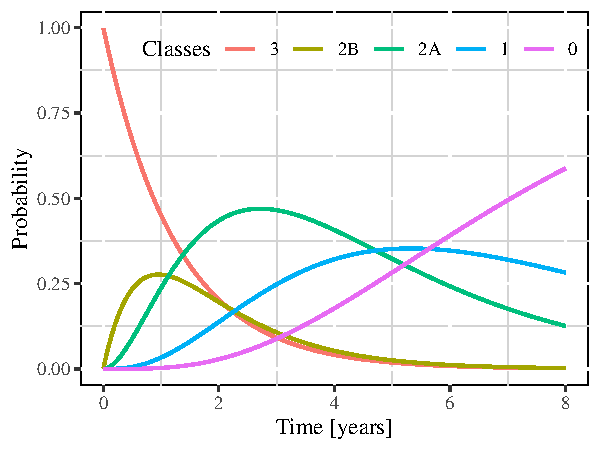
\includegraphics[width=0.475\textwidth]{trans_dist_gerlang.pdf}
            \includegraphics[width=0.475\textwidth]{tpm_dist_gerlang.pdf}
            \caption[]%
            {{\small Nearest class, that is $\bm{A}_{\RN{1}}$ in \cref{eq:generator_erlang}.}}   
            \label{fig:trans_dist_gerlang}
        \end{subfigure}
        \\ 
        \begin{subfigure}[t]{1 \textwidth}   
            \centering 
            \includegraphics[width=0.475\textwidth]{trans_dist_gerlang_relax.pdf}
             \includegraphics[width=0.475\textwidth]{tpm_dist_gerlang_relax.pdf}
            \caption[]%
            {{\small Relaxed Erlang, that is $\bm{A}_{\RN{2}}$ with mean degradation time following \cref{eq:trans_rate_param}.}}
            \label{fig:trans_dist_gerlang_relax}
        \end{subfigure}
        \\
        \begin{subfigure}[t]{1 \textwidth}  
            \centering 
            \includegraphics[width=0.475\textwidth]{trans_dist_tridiagonal.pdf}
             \includegraphics[width=0.475\textwidth]{tpm_dist_tridiagonal.pdf}
            \caption[]%
            {{\small Up to 3 classes ahead, that is $\bm{A}_{\RN{4}}$ in \cref{eq:generator_tridiagonal}.}}    
            \label{fig:trans_dist_tridiagonal}
        \end{subfigure} \\
        \caption{Left column: Transient distribution over time of the Markov jump process wrt. the parameterization of the generator. The initial distribution of the chain is $\bm{\pi}^{(s)}(0) = \begin{bmatrix}1 & 0 & 0 & 0 & 0 \end{bmatrix}$. Right column: Transition probability matrix, that is, the matrix exponential, $\exp\left(\bm{A}^{(s)}\tau'^{(s)}\right)$, where $\bm{A}^{(s)}$ refers to a chosen parameterization of the generator and $\tau'^{(s)}$ is eight years.}
        \label{fig:transient_dists}
    \end{figure*}

The first row of each TPM corresponds to the transient distribution after ten years. 
The standard MJP places the majority of probability mass in the absorbing class $0$ after ten years (\cref{fig:trans_dist_1}), whereas the MJP with state-dependent regression assigns most probability at class $1$ (\cref{fig:trans_dist_2}), but with substantially less sharpness (i.e. probabilities are more equally spread across classes). The mixture MJP approaches a state distribution \DIFdelbegin \DIFdel{that tends to evolve more statically }\DIFdelend \DIFaddbegin \DIFadd{which is more static }\DIFaddend after two years (\cref{fig:trans_dist_3}) than its counterparts.

\paragraph{Turning points in the evolution of class probabilities.} \label{sec:turning_points}
With upper triangular generators, the transient distribution of the standard MJP follows a simple principle: once a class probability starts to decrease, it will not increase again. This results in curves with at most one turning point, cf. \cref{fig:trans_dist_1}. 
This principle does not apply to the MJP with the state-dependent regression of \cref{eq:trans_rates_covariates2}, because as the observation interval increases, the expected proportion of time spent in each class (i.e. the weights $w_j^{(s)}$) changes. For instance, at small observation intervals, most weight will be placed on the starting class, whereas for longer observation intervals more weight will be placed on the more progressed classes.
Since the state-dependent regression depends on these weights by \cref{eq:trans_rates_covariates2} that again depend on the observation interval through \cref{eq:sojourn_time_estimate}, the resulting time-scaling $g(\eta^{(s)}) \tau^{(s)}$ is not necessarily monotonically increasing with $\tau^{(s)}$, because the coefficients $\bm \beta_j$ for every class $j \in \mathcal J$ will dominate according to the weights $w_j^{(s)}$ (so $g(\eta^{(s)})$ can decrease when $\tau^{(s)}$ increases).
Therefore, when the transient distribution is plotted against the observation interval, multiple turning points can occur, which is also evident in \cref{fig:trans_dist_2}. For instance, we see that the class $1$ probability increases rapidly during the first year, then it decreases slowly until year five, where it begins to increase again. Increasing the time horizon would reveal this class $1$ probability to finally approach zero, as the defect reaches the absorbing state.

\paragraph{The implications of different model specifications.}
The models specifications provide different ways to represent the degradation mechanisms. The transient distribution of the standard MJP offers an interpretation of the modeled degradation which is easily conveyable to practitioners: 
It models gradual progression of defects for all of the considered generators,
and it can also model the probability of shock events, by choosing a generator that allows multiple skips.
Comparing the transient distribution of $\bm{A}_{\RN{3}}$ in \cref{fig:trans_dist_1}, with the one that would arise from using $\bm{A}_{\RN{1}}$, one would see substantially more probability mass assigned to class $2B$, because $\bm{A}_{\RN{1}}$ would enforce defects to visit that class before progressing further, even though this class has few observations in the available data (see \cref{fig:hists_u}). Therefore, the standard MJP approach has the ability to adapt to unbalanced data through generator parameterization. 
The model with modified sojourn time estimates reveals the same structural behavior in the transient distribution as the standard MJP, but with higher flexility in how probability mass can be spread according to a modified ``process clock'' instead of calendar time.

The state-dependent regression offers a model extension to the standard MJP that models more complex dynamics between exogenous information and the response in transition behavior. The resulting transient distribution becomes more difficult to communicate, and it may not reflect the ``common sense'' understanding of degradation behavior as seen in \cref{fig:trans_dist_2}, as we described \cref{sec:turning_points}. However, it improves prediction accuracy substantially (cf. \cref{tab:prediction_scores}), compared to the global regression setting, and practitioners could argue for its use based on how well it fits data.

The transient distribution of the mixture MJP constitutes a weighed average of the transient distributions from $G$ MJPs, with transition rates and weights for the latent components jointly determined. With this model complexity, some would argue that it approaches model formulations seen in purely data-driven approaches. It is more difficult to communicate the degradation dynamics, as the latent components may not have a direct physical interpretation, but in the forecasting task it outperforms any other of the predictors (\cref{tab:prediction_scores}).


%The transient distribution is more stable over time,
%(the following section evaluates how well it approximates the transition behavior (independently from observation intervals) in the data).
%complex dependencies with exogeneous information
%how effective it approximates the empirical distribution


%%consider making a new subsection for transition residuals and covariate impact







%Because $\bm{A}_{\RN{1}}$ only allows jumps to neighboring classes, it assigns substantially more probability mass to class $2B$ (see \cref{fig:trans_dist_gerlang}) than $\bm{A}_{\RN{4}}$ (\cref{fig:trans_dist_tridiagonal}), which permits direct jumps to more severe categories without passing through all intermediate states.
%This difference likely reflects the relatively low number of observed class $2B$ defects, causing $\bm{A}_{\RN{4}}$ to assign little probability to that state over time.

%$\bm{A}_{\RN{2}}$ (\cref{fig:trans_dist_gerlang_relax}) assigns less probability mass to class $2B$ than $\bm{A}_{\RN{1}}$, but more than $\bm{A}_{\RN{4}}$. However, it differs notably from both in its treatment of the most severe classes: it assigns substantially more probability mass to class $1$ and correspondingly less to class $0$ after ten years.
%This shift stems from the core assumption of $\bm{A}_{\RN{2}}$ (\cref{eq:trans_rate_param}), where the degradation time between two observed states is modeled as the sum of intermediate sub-degradation processes.
%As a result, probability mass is systematically shifted toward intermediate states, leading to the observed leftward bias in the transition matrix compared to $\bm{A}_{\RN{1}}$ and $\bm{A}_{\RN{4}}$.





%While $\bm{A}_{\RN{1}}$ enforces gradual transitions between neighboring severity classes, it can still capture sudden defect propagation through rapid sequences of small jumps.Conversely, $\bm{A}_{\RN{4}}$ (as well as $\bm{A}_{\RN{3}}$ and $\bm{A}_{\RN{5}}$) allows direct jumps to more severe classes without passing through intermediates, making it well-suited for modeling abrupt failures caused by random shocks, such as those imposed by heavy rolling stock loads or external impacts. $\bm{A}_{\RN{2}}$ lies between these two extremes: it models large transitions as the cumulative effect of smaller degradation steps, combining gradual wear processes with the possibility of accelerated defect growth.

% Note that the first row in the transition probability matrices corresponds to the transient distribution after eight years. As the generalized Erlang only models jumps to the neighboring class, it assigns substantially more probability mass to class $2B$ (see \cref{fig:trans_dist_gerlang}) than the free upper parameterization in \cref{fig:trans_dist_free_upper}, which is not restricted to visit $2B$ before it can move further into more severe categories. Most likely, the relatively low number of $2B$ observations is the reason why the free upper parameterization from \cref{eq:generator_free_upper} assigns low probability to that state over the eight year period. The reparameterized upper in \cref{fig:trans_dist_param_upper} assigns less probability mass to category $2B$ than the generalized Erlang, but more than the free upper. However, the reparameterized upper from \cref{eq:trans_rate_param} differs notably from the two other parameterizations wrt. category $1$ and $0$ where it assigns significantly more probability mass to class $1$ than the generalized Erlang and the free upper. Most of this probability mass comes from class $0$ which has substantially lower probability mass after eight years than in the cases of the generalized Erlang and the free upper. This is caused by the core assumption of the reparameterized upper in \cref{eq:trans_rate_param}, where the degradation time between two observed states is the sum of all intermediate sub-degradation processes. In general, the assumption will force more probability mass to the left in the transition probability matrix, which indeed is the case in \cref{fig:trans_dist_param_upper} compared to \cref{fig:trans_dist_gerlang} or \cref{fig:trans_dist_free_upper}.
% Although, the free upper parameterization has the highest prediction accuracy, the reparameterized upper has its merits. The parameter spaces of the free upper increases quadratically with the number of categories in the state space, while it increases linearly for the reparameterized upper. For the fairly small state space considered in this present study ($m = 5$), model estimation appears robust. However, for larger state spaces it might be more problematic to robustly determine all parameters using the free upper parameterization. In that case, the reparameterized upper could offer an alternative with as few parameters as the generalized Erlang but with more flexibility for jumps in the Markov chain.

%\FloatBarrier

%\subsection{Exogenous information} \label{sec:results_exogenous_info}
%The inclusion of the exogenous information containing the track characteristics consistently improves prediction errors. This holds true for all investigated model settings of the cumulative link model and the Markov jump process. 
%This supports the notion of heterogeneity of the rail network, since taking the specific rail characteristics at the defect location into account leads to better predictions, see \cref{tab:forecast_error_tab}.
%\citet{bisgaard2024A} demonstrate that the included covariates are statistically significant on a 5\% level, computing the standard errors of the parameters via a second order approximation of the score function in the estimated optimum. Due to the $k$-fold cross validation procedure in this study, we obtain $k$ different estimates for each variable for each model setting. In \cref{tab:covariates_estimates}, we show the range of the coefficients.
%\begin{table}[htb!]
%    \centering
%    \caption{Model estimates of rail track characteristics from k-fold estimation procedure}
%    \centerline{\begin{tabular}[t]{>{}llccccc}
\toprule
 & Model & Tonnage & Line speed & Rail profile & Steel hardness & Curvature\\
\midrule
\addlinespace[0.3em]
\multicolumn{7}{l}{\textbf{\textbf{Cumulative link}}}\\
\hspace{1em} & Logistic link & {}[0.49, 0.66] & {}[0.03, 0.15] & {}[-1.15, -0.95] & {}[0.80, 0.91] & {}[0.48, 0.68]\\

\hspace{1em} & Probit link & {}[0.33, 0.42] & {}[0.01, 0.08] & {}[-0.72, -0.59] & {}[0.44, 0.49] & {}[0.28, 0.39]\\

\hspace{1em} & Cloglog link & {}[0.40, 0.50] & {}[-0.10, 0.01] & {}[-0.86, -0.68] & {}[0.42, 0.48] & {}[0.27, 0.40]\\
\cmidrule{1-7}
\addlinespace[0.3em]
\multicolumn{7}{l}{\textbf{\textbf{Markov jump process}}}\\
\hspace{1em} & Generalized Erlang, $\bm{A}'$ & {}[0.38, 0.49] & {}[0.30, 0.42] & {}[-0.86, -0.65] & {}[0.69, 0.78] & {}[0.45, 0.59]\\

\hspace{1em} & Reparameterized upper, $\bm{A}''$ & {}[0.57, 0.72] & {}[0.20, 0.31] & {}[-0.78, -0.58] & {}[0.69, 0.78] & {}[0.52, 0.65]\\

\hspace{1em} & Free upper, $\bm{A}'''$ & {}[0.57, 0.69] & {}[0.15, 0.25] & {}[-0.61, -0.41] & {}[0.65, 0.74] & {}[0.58, 0.71]\\
\bottomrule
\end{tabular}}
%    \label{tab:covariates_estimates}
%\end{table}
%For all folds, the coefficients on the covariates have constant sign and are of similar magnitude, with the only exception of the complementary loglog link for the cumulative link model. However as shown in \cref{tab:forecast_error_tab}, the complementary loglog link has the worst prediction performance of all investigated parametric models, suggesting that the assumption of a min-Gumbell distributed latent variable is not suitable. With that aside, the fact that different settings (link functions and generator parameterizations) of two distinct statistical models lead to similar estimated coefficients for the covariates on all studied subsets of the data strongly suggests that the estimations are robust and that the statistical interpretation of the influence of the covariates is sound. We conclude that the models associate increases in tonnage, line speed, steel hardness and curvature with faster propagation of defect severity. Increasing rail profile is associated with slower propagation of defect severity. As argued by \citet{bisgaard2024A}, these associations are in accordance with railway domain knowledge \citep{UIC_2002_defecthandbook,RASMUSSEN20178}


\subsubsection{Transition residuals} \label{sec:transition_patterns}

To compare the model-implied transitions with the empirical ones, define the elements in the transition count matrix
$
  N_{i,j}^{\text{obs.}} = \sum_{s \in \mathcal S} \mathds{1}_{y_1^{(s)} =\; i, y_2^{(s)} =\; j}
$ for $i,j \in \mathcal J$, which express the number of observed transitions from state $i$ to $j$. The expected transition counts implied by a model predicting a transient distribution $\widehat{\bm \pi}^{(s)}$ at the time of the second observation is given by
$
\widehat{  N}_{i,j} =  \sum_{s \in \mathcal S} \mathds{1}_{y_1^{(s)} = \; i} \widehat{ \pi}_j^{(s)},
$ for $i,j \in \mathcal J$.
Then, the transition residuals for a model can be calculated as
\DIFdelbegin %DIFDELCMD < $$
%DIFDELCMD <   R_{i,j} = \left(  N_{i,j}^{\text{obs.}} - \widehat{  N}_{i,j} \right) / \sum_{j}   N_{i,j}^{\text{obs.}},
%DIFDELCMD < $$%%%
\DIFdelend \DIFaddbegin $$
  R_{i,j} = \left(  N_{i,j}^{\text{obs.}} - \widehat{  N}_{i,j} \right) / \sum_{j}   \widehat{  N}_{i,j},
$$\DIFaddend  for $i,j \in \mathcal J$.
The entries, $  R_{i,j}$, express the error between the observed number of transitions from state $i$ to $j$, and the expected counts implied by the model predictions, in proportions. 
By construction, $\sum_{j}   R_{i,j} = 0$, so if $  R_{i,j} > 0$, the model underpredicts the amount of $i$ to $j$ transitions, and vice versa for $  R_{i,j} < 0$.
Thus, inspecting $\bm R$ (comprised by the elements $R_{i,j}$) for a model can serve as check of how well it approximates the empirical distribution of the transition patterns between starting and ending state. The norm of $\bm R$ can be used as simple diagnostic for this check, e.g. taking the L1-norm of the transition residuals
$
|| \bm R || = \sum_{i,j} |  R_{i,j}|
$ for $i,j \in \mathcal J$.

For each predictor, we calculate $\bm R$ based on the held-out set in the CV described in \cref{sec:prediction_error}, then aggregating across the folds. In \cref{tab:transition_patterns}, three of these $\bm R$'s are displayed for the MJP under the $\bm{A}_{\RN{3}}$ parameterization with the different covariate setting in \cref{sec:regression} (\cref{tab:expected_transition_bidiagonal_cov1_exp_exp_all_no_warp}, respectively \cref{tab:expected_transition_bidiagonal_cov2_exp_exp_all_no_warp}), and a mixture model using four generators (\cref{tab:expected_transition_bidiagonal_cov1_exp_exp_all_no_warp_mixture4}). As a reference check of the empirical distribution of the $i$ to $j$ transitions, the empirical row-normalized transition matrix, $ N_{i,j}^{\text{obs.}} / \sum_{j}  N_{i,j}^{\text{obs.}}$, is included (\cref{tab:transition_matrix}).

\begin{table}[h]
    \begin{subtable}[h]{0.45\textwidth}
        \centering
            \input{transition_matrix}
          \caption{Transition matrix, $ N_{i,j}^{\text{obs.}} / \sum_{j}  N_{i,j}^{\text{obs.}}$.}
       \label{tab:transition_matrix}
    \end{subtable}
    \hfill
    \begin{subtable}[h]{0.45\textwidth}
        \centering
       \input{expected_transition_bidiagonal_cov1_exp_exp_all_no_warp}
        \caption{$\bm R$ given $\bm{A}_{\RN{3}}$ with global regression (\cref{eq:trans_rates_covariates}).}
        \label{tab:expected_transition_bidiagonal_cov1_exp_exp_all_no_warp}
     \end{subtable}
      \begin{subtable}[h]{0.45\textwidth} 
        \centering
         \input{expected_transition_bidiagonal_cov2_exp_exp_all_no_warp}
        \caption{$\bm R$ given $\bm{A}_{\RN{3}}$ with state-dependent regression (\cref{eq:trans_rates_covariates2}).}
        \label{tab:expected_transition_bidiagonal_cov2_exp_exp_all_no_warp}
     \end{subtable}
     \hfill 
     \begin{subtable}[h]{0.45\textwidth} 
        \centering 
 \input{expected_transition_bidiagonal_cov1_exp_exp_all_no_warp_mixture4}
        \caption{$\bm R$ given mixtures of $\bm{A}_{\RN{3}}$ (\cref{sec:mixture} with $G = 4$) and global regression (\cref{eq:trans_rates_covariates}).}
        \label{tab:expected_transition_bidiagonal_cov1_exp_exp_all_no_warp_mixture4}
     \end{subtable} 
     \caption{Transition residuals comparing model-implied and empirical transitions.}
     \label{tab:transition_patterns}
\end{table}


As seen from the proportions in \cref{tab:transition_matrix}, there is a substantial amount of transitions appearing over more than one class ahead. Overall, the $\bm{A}_{\RN{3}}$ with state-dependent covariates (\cref{tab:expected_transition_bidiagonal_cov2_exp_exp_all_no_warp}) improves the residuals compared to the setting with global regression coefficients (\cref{tab:expected_transition_bidiagonal_cov1_exp_exp_all_no_warp}), as indicated by a lower L1-norm (0.385 vs 0.327). Both settings have their largest residuals in the $1 \rightarrow 0$ transition and overpredict the probability of reaching the absorbing state (class $0$). Clearly, the mixture model matches the empirical transition frequencies more closely (\cref{tab:expected_transition_bidiagonal_cov1_exp_exp_all_no_warp_mixture4}), with an L1-norm of approx. 0.020, which is expected given its flexibility in adapting to data. In contrast, the single-generator MJP settings are more constrained by the assumed degradation mechanism, while the observed transition data may be influenced by practices and policies that prevent many defects from progressing to rail breaks once they reach a safety-critical level (e.g., class $1$).

Appendix \ref{sec:transition_L1} provides a full summary of the L1-norms of the $\bm R$'s from all outlined predictors.




\subsubsection{The impact of the covariates: An example} \label{sec:risk_curves}
In practice, infrastructure managers could be interested in quantifying the impact of the covariates on the risk of obtaining a critical defect. We here provide an example of how this can be done within the existing model framework.
Define the critical class set $\mathcal E_{\text{critical}} = \{ 1,0\}$ with corresponding index set $\mathcal J_{\text{critical}}$. Further, we define the associated critical curve
$$
r^{(s)}(t) = \mathds P\left(X^{(s)}(t) \in \mathcal J_{\text{critical}} \mid X^{(s)}(0) = y_1^{(s)}, \bm z^{(s)}\right) = \sum_{j\in \mathcal J_{\text{critical}}} \widehat{\pi}_j^{(s)}(t; \bm z^{(s)}), 
$$
where $\widehat{\bm \pi}^{(s)}(t; \bm z^{(s)})$ is the predicted distribution for defect $s \in \mathcal S$ at time $t$ with covariates $\bm z^{(s)}$.

To exemplify how covariates impact the risk curve $r^{(s)}(t)$, we consider an MJP with a regression setting. For this example, we use the $\bm{A}_{\RN{3}}$ generator with state-dependent regression coefficients (\cref{eq:trans_rates_covariates2}) and set $y_1^{(s)}$ equal to class $3$. Three scenarios are then computed for a single covariate $\bm z_k \in \bm z$, that is the empirical 10\%, 50\%, and 90\% quantiles across the defects in the dataset, while the empirical means are computed for the remaining covariates. 
For each scenario, we then compute $r^{(s)}(t)$ over a five-year horizon for the variables tonnage, curvature, and rail weight. These risk curves are presented in \cref{fig:critical_curves}\DIFaddbegin \DIFadd{, so that covariate-dependency is reflected through the quantiles}\DIFaddend .

\begin{figure}[htb!]
  \centering
\begin{subfigure}{.33\textwidth}
  \centering
  \includegraphics[width=\linewidth]{crit_curves_1}
  \caption{Tonnage}
  \label{fig:crit_curves_1}
\end{subfigure}%
\begin{subfigure}{.33\textwidth}
  \centering
  \includegraphics[width=\linewidth]{crit_curves_5}
  \caption{Curvature}
  \label{fig:crit_curves_5}
\end{subfigure}
\begin{subfigure}{.33\textwidth}
  \centering
  \includegraphics[width=\linewidth]{crit_curves_3}
  \caption{Rail weight}
  \label{fig:crit_curves_3}
\end{subfigure}
\caption{Risk curves $r^{(s)}(t)$ under varying impacts of covariates using an MJP with $\bm{A}_{\RN{3}}$ generator and state-dependent regression coefficients (\cref{eq:trans_rates_covariates2}).}
\label{fig:critical_curves}
\end{figure}

From \cref{fig:crit_curves_1} and \cref{fig:crit_curves_5}, we see that the model associates high tonnage and curvature values with higher risk of reaching $\mathcal J_{\text{critical}}$, in line with existing domain knowledge that increasing intensity of traffic increases defect progression. \cref{fig:crit_curves_3} indicates that bigger rail profiles lower the risk of a defect progression into a critical class.
In summary,  the resulting curves provide a simple, decision-relevant visualization of how changes in covariates shift the predicted probability of reaching a critical defect class (given a model specification) over time. 


\subsection{Calibration, discrimination, and sharpness} \label{sec:reliability_analysis}
The proper scoring rules in \cref{sec:prediction_error} showed that the flexible MJP parameterizations outperform the reference predictors (most substantially the mixture MJPs), and that modifying sojourn time estimates, exogenous information, and averaging over all predictors in an ensemble improve accuracy.
However, such scores reduce forecast quality to single summary values, and therefore cannot reveal the specific sources of deficiencies \citep{hamill1997,Dimitriadis_2024}. So far, we supplemented this evaluation by inspecting transition residuals (\cref{sec:transition_patterns}), but to provide a more detailed analysis, multicategorical reliability diagrams are generated to assess forecast calibration, and checkerboard plots to evaluate discrimination ability.\footnote{Our GitHub repository (\url{https://github.com/dobbeltgaard/MarkovJump.git}) provides \texttt{R} code to generate these diagnostic plots.} Also, the sharpness of the predictors will be assessed using an entropy measure. 

\subsubsection{Multicategory reliability diagrams}
We follow the methodology proposed by \citet{hamill1997}, extending the framework of reliability diagrams initially introduced for binary forecasts by \citet{wilks1995a}.
The diagnostic plots are generated by the following procedure.
\begin{enumerate}    
    \item Define a set of quantiles $q_1, q_2, \dots, q_K$ (e.g., $0.05, 0.15, \dots, 0.95$), where $K$ is the number of quantiles.
    \item For each forecast, compute the cumulative probabilities across the $m$ categories. For each quantile $q_k$, determine the forecasted category as the smallest category where the cumulative probability exceeds or equals $q_k$. This converts the probabilistic forecasts into categories at each quantile.
    \item For each forecast-observation pair, the multicategory reliability is defined as:
    \begin{itemize}
        \item $1$ if the observed category is less than the forecasted category.
        \item $0$ if the observed category is greater than the forecasted category.
        \item $\frac{q - q_{\min}}{q_{\max} - q_{\min}}$ if the observed category equals the forecasted category, where $q_{\min}$ and $q_{\max}$ are the quantiles where the observation matches the forecast.
    \end{itemize}
    \item For each quantile $q_k$, compute the average reliability across all forecast-observation pairs.
\end{enumerate}
As a supplementary summary metric, we report the \textit{average category error}, defined as the mean absolute difference between the forecasted category at each quantile and the observed category, averaged first across forecasts and then across quantiles.

Error bars are calculated via a bootstrap procedure, which repeats the above steps across multiple resampled datasets. A checkerboard plot of the difference between the forecasted and observed categories at each quantile is used to visualize the discrimination ability of the forecasts. \citet{hamill1997} offers an exhaustive description of the above methodology.

\subsubsection{Entropy measure}
To assess forecast sharpness, we define for a predicted distribution $\widehat{\bm\pi}^{(s)}$ a normalized entropy measure by
\begin{align}
H(\widehat{\bm\pi}^{(s)}) = - \frac{1}{\log m}\sum_{j=1}^{m}\widehat{\pi}^{(s)}_j \log\!\big(\widehat{\pi}^{(s)}_j\big), \quad s \in \mathcal S.\label{eq:entropy}
\end{align}
This quantifies the average level of uncertainty that a prediction assigns over the categories with $H \in [0,1]$, so that the sharper a forecast is, the lower $H$ becomes.

\subsubsection{Summary of calibration, discrimination, and sharpness}
Based on the out-of-fold predictions from the CV procedure in \cref{sec:prediction_error}, the multicategory reliability diagrams with checkerboard plots are generated, so each defect contributes once. Further, we report mean predictive entropy as a measure of sharpness, computed for each held-out forecast and averaged (a full list is provided in Appendix \ref{sec:sharpness}).

To illustrate, we focus on four predictors: 
1) the uniform predictor; 
2) the logistic CLM with exogenous information; 
3) the MJP with parameterization $\bm{A}_{\RN{3}}$ including exogenous information;
4) and the MJP mixture using the $\bm{A}_{\RN{3}}$ parameterization including exogenous information. 
Bootstrapping was performed with 200 resamples, and 10\% and 90\% confidence intervals are reported. We use $K = 10$ quantiles ($0.05, 0.15, \dots, 0.95$). Results are shown in \cref{fig:reliability_diagrams}.
Note that wider uncertainty bands at the highest quantiles can reflect lower effective sample sizes, particularly for rare class $0$ transitions. We found 200 resamples sufficient for stable curves in repeated runs.



 \begin{figure*}[htb!]
        \centering
        \begin{subfigure}[t]{0.475\textwidth}
            \centering
            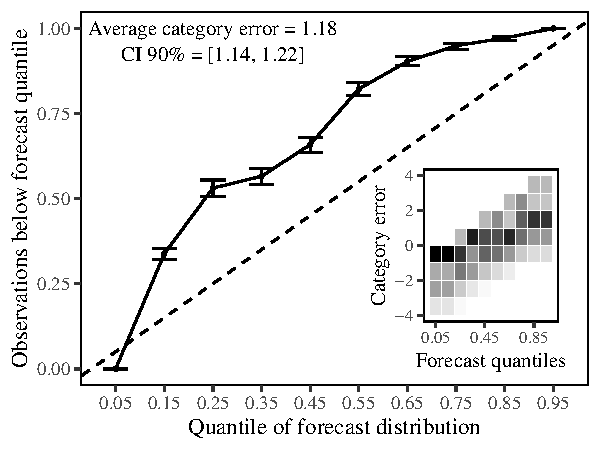
\includegraphics[width=\textwidth]{reliability_diag_uniform.pdf}
            \caption[]%
            {{\small Uniform distribution predictor from \cref{eq:uniform_predictor}}}    
            \label{fig:reliability_diag_uniform}
        \end{subfigure}
        \hfill
        \begin{subfigure}[t]{0.475\textwidth}  
            \centering 
            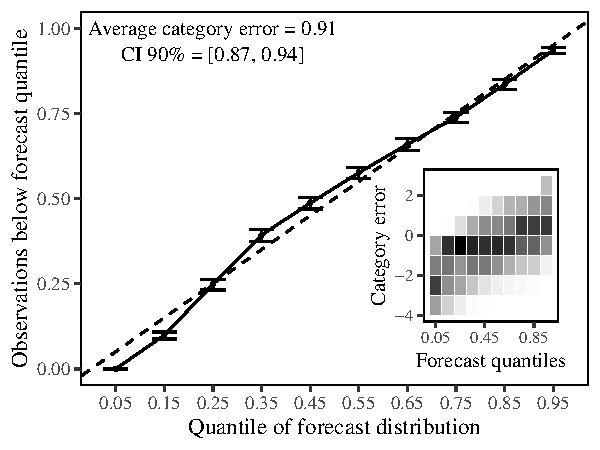
\includegraphics[width=\textwidth]{reliability_diag_olr_cov.pdf}
            \caption[]%
            {{\small Cumulative logistic link with exogenous information}}    
            \label{fig:reliability_diag_olr_cov}
        \end{subfigure}
        \hfill
        \begin{subfigure}[t]{0.475\textwidth}   
            \centering 
            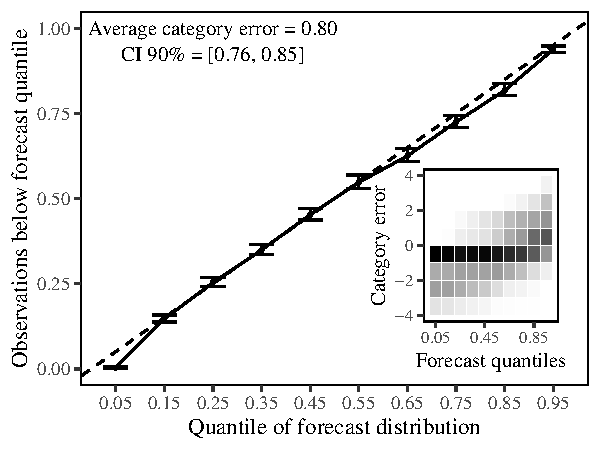
\includegraphics[width=\textwidth]{reliability_diag_bidiagonal_TRUE_exp_exp_all_warp.pdf}
            \caption[]%
            {{\small Up to 2 classes ahead with exogenous information and modified sojourn time estimates, that is $\bm{A}_{\RN{3}}$ in \cref{eq:generator_bidiagonal} using \cref{eq:trans_rates_covariates} and \cref{eq:warped_time}.}}    
            \label{fig:reliability_diag_bidiagonal_TRUE_exp_exp_all_warp}
        \end{subfigure}
        \hfill
        \begin{subfigure}[t]{0.475\textwidth}   
            \centering 
            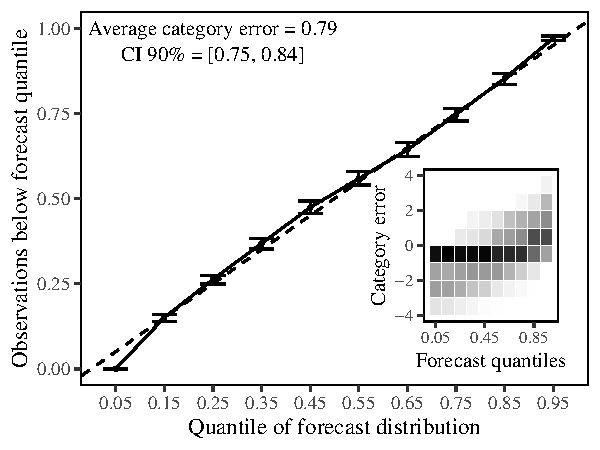
\includegraphics[width=\textwidth]{reliability_diag_ensemble_all.pdf}
            \caption[]%
            {{\small Ensemble}}    
            \label{fig:reliability_diag_ensemble_all}
        \end{subfigure}
        \caption{Multicategorical reliability diagrams showing the fraction of observations below the forecast quantile. We use 10 quantiles, that is ($0.05, 0.15, \dots, 0.95$). The dotted line represents a perfectly calibrated forecast. Error bars are calculated using bootstrap testing. Inset checkerboard plots show the average category error wrt. the quantiles. Highly populated bins are darker colored. Perfect forecasts have 0 category error.}
        \label{fig:reliability_diagrams}
    \end{figure*}


The uniform distribution predictor (\cref{fig:reliability_diag_uniform}) substantially overestimates the fraction of observed categories across all quantiles, indicating high miscalibration.
Its average category error is also the highest among the four predictors, consistent with its poor performance on aggregate scores in \cref{tab:prediction_scores}. Its average normalized entropy is $0.8093$, which is expected since a uniform predictor is preferenceless, meaning it has minimal sharpness.\footnote{Remark the only reason it does not attain the maximum value of $1$ for the average entropy is that \cref{eq:uniform_predictor} only spreads out probability mass to the states that are reachable given the initial observation $y_1^{(s)}$ (if the support size is $r<m$, the maximum normalized entropy becomes $\log(r)/\log(m) < 1$).}

The cumulative link model with logistic link (\cref{fig:reliability_diag_olr_cov}) shows improvement in calibration relative to the uniform distribution predictor.
Its discrimination ability remains modest, as indicated by large average category errors and checkerboard plots with heavily populated bins far from the zero-error line. Average entropy is large ($0.7416$).

The MJP (\cref{fig:reliability_diag_bidiagonal_cov1_exp_exp_all_no_warp}) achieves the lowest mean category error among the single predictors, and its checkerboard plot shows concentration of errors near the zero-category line, indicating good discrimination ability.
Its reliability curve indicates that it tends to underpredict severity, most noticeably at higher quantiles.
The mixture MJP (\cref{fig:reliability_diag_bidiagonal_cov1_exp_exp_all_no_warp_mixture4}) has larger mean category error, but better calibrated forecasts at the higher quantiles (cf. \cref{sec:transition_patterns}, where it better matches empirical transition frequencies). However, it has weakened discrimination ability at the higher quantiles (see the darker bins away from zero at the two last bins in the checkerboard), indicating a trade-off between calibration and discrimination ability.
The entropy of the single generator MJP is $0.5249$ compared to $0.5857$ for the mixture MJP, which suggests that the mixture MJP is more conservative in how it distributes the probability mass (also reflected in slower evolution of the rail break risk in \cref{sec:results_transient_dist_markov}). As the mixture MJP was the predictor with the highest predictive accuracy in terms of RPS and log score, it suggests that a loss of sharpness can be beneficial if it improves calibration enough.



\subsection{Proposition for use case} \label{sec:proposition_for_use}
From the perspective of an infrastructure manager, probabilistic forecasts in isolation have limited operational value. 
For better network operation, forecasts must be embedded in decision frameworks that allocate resources under uncertainty.\footnote{Discussions with BaneNOR and Banedanmark (the infrastructure managers responsible for most of the Norwegian and Danish networks) highlighted that connecting predictions to actionable maintenance strategies is essential for realizing the value of predictive models.}
%One possible implementation pathway could be threshold-based decisions under a fixed budget: for each defect, generate forecasts over a six-month horizon and allocate resources to the $n$ defects with the highest probability of reaching a critical state, with $n$ bounded by the budget divided by the average per-defect action cost. Such a heuristic is unlikely to lead to near-optimal network operation, because it ignores the value of information from inspection and the timing of decisions over multiple horizons.
In the following, we outline and solve a stochastic program that connects probabilistic forecasts to sequential inspection and maintenance decisions over multiple stages. \DIFaddbegin \DIFadd{This example is intended as a proof-of-concept rather than a fully operational maintenance planning tool (cf. \cref{sec:conclusion}).
}\DIFaddend 


\subsubsection{A stochastic program}
Here, we formulate an optimization model that, based on the predictions, minimizes expected cost over a time horizon of $T_n$ related to active defects in a set $\mathcal{S}$ across a railway network with a rail line mapping $\ell:\mathcal{S}\to\{\text{rail lines}\}$.


\paragraph{Decision variables and available information.}
We will consider maintenance and inspection planning on a time grid $\widehat T=(T_1,\dots,T_n)$.
At these time points (stages), we define decision variables 
$y^{(s)}(t)\in\{0,1\}$ for inspection and \DIFdelbegin \DIFdel{$z^{(s)}(t)\in\{0,1\}$ }\DIFdelend \DIFaddbegin \DIFadd{$w^{(s)}(t)\in\{0,1\}$ }\DIFaddend for maintenance at time $t \in \widehat T$ for defect $s\in\mathcal S$.
%$$
%y^{(s)}(t)\in\{0,1\}\quad\text{(inspection at \(T_t\))}, \qquad %\text{and }
%z^{(s)}(t)\in\{0,1\}\quad\text{(maintenance at \(T_t\))},
%$$
%for $t = 1, \dots, n$.
The information available to the infrastructure manager is represented by the $\sigma$-algebra generated by the outcomes of decisions made so far, that is, a filtration
\DIFdelbegin \DIFdel{$
\mathcal F(t) = \sigma \left( O^{(s)}(\tau), y^{(s)}(\tau), z^{(s)}(\tau) : \tau \leq t, s\in\mathcal S \right), 
$
}\DIFdelend \DIFaddbegin \DIFadd{$
\mathcal F(t) = \sigma \left( O^{(s)}(\tau), y^{(s)}(\tau), w^{(s)}(\tau) : \tau \leq t, s\in\mathcal S \right), 
$
}\DIFaddend for $t = 1, \dots, n$ with the observation process 
$$
O^{(s)}(t) = \begin{cases}
X^{(s)}(t), \quad &y^{(s)}(t) = 1\\ 
\varnothing, \quad &y^{(s)}(t) = 0.
\end{cases}
$$
Note that at each stage $t$, the predicted distributions $\widehat{\bm \pi}^{(s)}(t \mid \mathcal F(t))$ are computed given the information available in $\mathcal F(t)$, and so they are $\mathcal F(t)$-measurable.

We let the indicator \(a^{(s)}(t)\in\{0,1\}\) express that defect \(s\) is still active, which means not maintained yet. We define \(\chi^{(s)}(t)\in\{0,1\}\) as an indicator that defect \(s\) is still uninspected. Subsequently, $a^{(s)}(t)$ and $\chi^{(s)}(t)$ are auxiliary variables that will help us write up the optimization program compactly.


\paragraph{Costs and critical class risks.}
Let the inspection cost at line $\ell$ be denoted by $c_{\text{ins}}^{\ell(s)}$, and $c_{\text{fail}}^{\ell(s)}$ the estimated costs of a rail break for $s \in \mathcal S$.
The expected maintenance cost is defined as 
$
\bar c^{(s)}(t) = \mathds E \left[ c_{\text{maint}}^{\ell(s)} \left(X^{(s)}(t)\right) \mid \mathcal F(t) \right]
$ where $c^{\ell(s)}_{\text{maint}}(j)$ is the maintenance cost for severity class $j$. \DIFaddbegin \DIFadd{The planned budget size is denoted $B(T_k)$ for period $T_k$.
}\DIFaddend 

Further, we define a critical-state probability, i.e., 
$
q^{(s)}(t) = \mathds P\left(X^{(s)}(t) \in \mathcal J_{\text{critical}} \mid \mathcal F(t) \right)
$ 
where $\mathcal J_{\text{critical}}$ for example can be defined as in \cref{sec:risk_curves}.
Before inspection, $\bar c^{(s)}(t)$ and $q^{(s)}(t)$ are forecast-based; after inspection, they are conditional on the observed class.

\paragraph{The objective function and constraints.}
The multistage stochastic program can then be written as a minimization of the expected costs, that is,
\DIFdelbegin %DIFDELCMD < \begin{align}
%DIFDELCMD < \min_{y,z,a,\chi}\quad
%DIFDELCMD < \mathbb E\!\left[
%DIFDELCMD < \sum_{k=1}^n\sum_{s\in\mathcal S}
%DIFDELCMD < \Bigl(
%DIFDELCMD < c_{\mathrm{ins}}^{\ell(s)} y^{(s)}(T_k)
%DIFDELCMD < + \bar c^{(s)}(T_k) z^{(s)}(T_k)
%DIFDELCMD < + c_{\mathrm{fail}}^{\ell(s)}\,q^{(s)}(T_k)\bigl(a^{(s)}(T_k)-z^{(s)}(T_k)\bigr)
%DIFDELCMD < \Bigr)
%DIFDELCMD < \right]
%DIFDELCMD < \label{eq:general_textbook_obj}
%DIFDELCMD < \end{align}%%%
\DIFdelend \DIFaddbegin \begin{align}
\min_{y,w,a,\chi}\quad
\mathbb E\!\left[
\sum_{k=1}^n\sum_{s\in\mathcal S}
\Bigl(
c_{\mathrm{ins}}^{\ell(s)} y^{(s)}(T_k)
+ \bar c^{(s)}(T_k) w^{(s)}(T_k)
+ c_{\mathrm{fail}}^{\ell(s)}\,q^{(s)}(T_k)\bigl(a^{(s)}(T_k)-w^{(s)}(T_k)\bigr)
\Bigr)
\right]
\label{eq:general_textbook_obj}
\end{align}\DIFaddend 
subject to
\DIFdelbegin %DIFDELCMD < \begin{align}
%DIFDELCMD < \sum_{s\in\mathcal S}
%DIFDELCMD < \Bigl(
%DIFDELCMD < c^{\ell(s)}_{\mathrm{ins}} y^{(s)} (T_k)
%DIFDELCMD < + \bar c^{(s)}(T_k) z^{(s)}(T_k)
%DIFDELCMD < \Bigr)
%DIFDELCMD < &\le B(T_k)
%DIFDELCMD < \qquad \text{a.s.},\quad k = 1,\dots,n,
%DIFDELCMD < \label{eq:general_textbook_budget}\\
%DIFDELCMD < y^{(s)}(T_k)+z^{(s)}(T_k)
%DIFDELCMD < &\le a^{(s)}(T_k)
%DIFDELCMD < \qquad \text{a.s.},\quad s\in\mathcal S,\  k = 1,\dots,n,
%DIFDELCMD < \label{eq:general_textbook_exclusive}\\
%DIFDELCMD < y^{(s)}(T_k)
%DIFDELCMD < &\le \chi^{(s)}(T_k)
%DIFDELCMD < \qquad \text{a.s.},\quad s\in\mathcal S,\  k = 1,\dots,n,
%DIFDELCMD < \label{eq:general_textbook_inspection}\\
%DIFDELCMD < a^{(s)}(T_1)&=1,\quad \chi^{(s)}(T_1)=1,
%DIFDELCMD < \qquad s\in\mathcal S,
%DIFDELCMD < \label{eq:general_textbook_initial}\\
%DIFDELCMD < a^{(s)}(T_{k+1})&=a^{(s)}(T_k)-z^{(s)}(T_k)
%DIFDELCMD < \qquad \text{a.s.},\quad s\in\mathcal S,\ k=1,\dots,n-1,
%DIFDELCMD < \label{eq:general_textbook_activity}\\
%DIFDELCMD < \chi^{(s)}(T_{k+1})&=\chi^{(s)}(T_k)-y^{(s)}(T_k)
%DIFDELCMD < \qquad \text{a.s.},\quad s\in\mathcal S,\ k=1,\dots,n-1.
%DIFDELCMD < \label{eq:general_textbook_uninspected}
%DIFDELCMD < \end{align}%%%
\DIFdelend \DIFaddbegin \begin{align}
\sum_{s\in\mathcal S}
\Bigl(
c^{\ell(s)}_{\mathrm{ins}} y^{(s)} (T_k)
+ \bar c^{(s)}(T_k) w^{(s)}(T_k)
\Bigr)
&\le B(T_k),\quad k = 1,\dots,n,
\label{eq:general_textbook_budget}\\
y^{(s)}(T_k)+w^{(s)}(T_k)
&\le a^{(s)}(T_k),\qquad s\in\mathcal S,\  k = 1,\dots,n,
\label{eq:general_textbook_exclusive}\\
y^{(s)}(T_k)
&\le \chi^{(s)}(T_k),\qquad s\in\mathcal S,\  k = 1,\dots,n,
\label{eq:general_textbook_inspection}\\
a^{(s)}(T_1)&=1,\qquad \chi^{(s)}(T_1)=1, \qquad s\in\mathcal S,
\label{eq:general_textbook_initial}\\
a^{(s)}(T_{k+1})&=a^{(s)}(T_k)-w^{(s)}(T_k),\qquad s\in\mathcal S,\ k=1,\dots,n-1,
\label{eq:general_textbook_activity}\\
\chi^{(s)}(T_{k+1})&=\chi^{(s)}(T_k)-y^{(s)}(T_k),\qquad s\in\mathcal S,\ k=1,\dots,n-1.
\label{eq:general_textbook_uninspected}
\end{align}\DIFaddend 
%All decision variables and auxiliary state variables are required to be \(\mathcal F_t\)-measurable at stage \(t\). 
The objective in \cref{eq:general_textbook_obj} combines inspection cost, expected maintenance cost, and expected failure cost. 
%Note that $q^{(s)}(t)$ lumps the forecast distribution into a stage-wise critical risk that enters as expected failure exposure for active defects. 
\cref{eq:general_textbook_budget}--\cref{eq:general_textbook_inspection} ensure budget feasibility\DIFaddbegin \footnote{\DIFadd{The budget constraint is imposed in expectation, so it should here be interpreted as a planning budget constraint rather than a hard realized budget constraint.}} \DIFaddend and at most one action per active defect and stage.
\cref{eq:general_textbook_initial}--\cref{eq:general_textbook_uninspected} ensure that the auxiliary variable are updated, so that maintenance removes a defect from the future decision stage and inspections update the information available for later decisions.\DIFdelbegin \footnote{\DIFdel{If an event has probability 1, then we say that this event occurs ``almost surely'' (a.s.) \citep[Chapter 3]{thygesen2023a}.}}
%DIFAUXCMD
\addtocounter{footnote}{-1}%DIFAUXCMD
\DIFdelend %DIF > \footnote{If an event has probability 1, then we say that this event occurs ``almost surely'' (a.s.) \citep[Chapter 3]{thygesen2023a}.}
\DIFaddbegin \DIFadd{Note that this model formulation can be extended to include further operational constraints, such as crew availability, possession windows, travel logistics, etc.
}\DIFaddend 


\subsubsection{Solving a stochastic program: An example}
To solve a stochastic program like \cref{eq:general_textbook_obj}--\cref{eq:general_textbook_uninspected}, uncertainty is typically represented by generating scenarios structured in a decision tree.
Given $m$ severity classes, $n$ decision stages, and $|\mathcal S|$ defects, the number of latent degradation paths is in the order of $m^{n|\mathcal S|}$.
Because the information available to the decision-maker depends on what is revealed by inspections, the optimization problem is subject to \textit{endogeneity}, 
%the uncertainty is \textit{endogenous}, 
meaning that the filtration $\mathcal F(t)$ depends on the inspection decisions $y^{(s)}(\tau)$ for $\tau\le t$, which increases the number of information branches.
This means that the optimization problem very quickly becomes intractable for increasing numbers of defects and decision stages.
Therefore, we have to approximate the full decision tree by a smaller one.


\paragraph{Numerical solution.}
First, for $10$ selected defects we generate Monte Carlo scenarios on a three-stage grid $(T_1,T_2,T_3)$ with known severity classes at $T_0$.\footnote{First-stage decisions will therefore be made at $T_1$.}
This is done over a $1.5$ year horizon using transition probabilities from a fitted MJP with $\bm{A}_{\RN{3}}$-generator and regression (\cref{eq:trans_rates_covariates}). 
Second, we reduce these sampled scenarios by using stage-wise clustering of the joint states at $T_2$ and $T_3$.
Endogenous information is handled by letting an inspection reveal the realized class at the decision stage. In later stages, the quantities $q^{(s)}(t)$ and $\bar c^{(s)}(t)$ are then computed conditional on the observed class; if no inspection is made, they are computed from the forecast distributions. More details are provided in Appendix \ref{sec:stochastic_optimization_details}.
\cref{tab:decisions} displays the obtained first-stage decisions.
\begin{table}[htb!]
\centering
\caption{First-stage decisions in the obtained policy.} \label{tab:decisions}
\begin{tabular}{clcl}
\toprule
Defect & Class at $T_0$ & \(q_{\mathrm{break}}(T_1)\) & Stage-1 decision \\
\midrule
1 & Class $3$ & 0.0346 & Inspect \\
2 & Class $2A$ & 0.1564 & Maintain \\
3 & Class $3$ & 0.0285 & Inspect \\
4 & Class $2A$ & 0.0677 & Wait \\
5 &Class $3$ & 0.0165 & Inspect \\
6 & Class $3$ & 0.0286 & Wait \\
7 & Class $2A$ & 0.0912 & Wait \\
8 & Class $2B$ & 0.0747 & Maintain \\
9 & Class $2A$ & 0.0993 & Maintain \\
10 & Class $2A$ & 0.1182 & Maintain \\
\bottomrule
\end{tabular}
\end{table}
As seen, the defects with lower severity are either assigned an inspection or no action, while the more progressed defects are assigned maintenance.


Taking defects 5 and 6 as a small case study, we see that defect 5 is inspected while defect 6 is not, even though both start in class $3$. The normalized entropy (\cref{eq:entropy}) of the one-step forecast at $T_1$ is $0.48$ for defect 5 and $0.66$ for defect 6, so defect 6 has the less sharp forecast at the first stage. %However, the policy is not driven by forecast uncertainty alone: inspection is only valuable if it is likely to change downstream actions.
In our solved policy (not fully shown in \cref{tab:decisions}), defect 6 is scheduled for maintenance at $T_2$ in a large fraction of the scenarios (about $71\%$), whereas defect 5 is maintained at $T_2$ much less often (about $34\%$). In other words, defect 6 is ``almost maintained anyway'', so paying for an inspection rarely changes the decision path. This illustrates how the program trades off inspection cost against the expected value of information.


%> entropy(t(c(1,0,0,0,0)) %*% TPMS[[3]]$TPM$dt_0.5)
%[1] 0.6570918
%> entropy(t(c(1,0,0,0,0)) %*% TPMS[[5]]$TPM$dt_0.5)
%[1] 0.4813692
%> entropy(t(c(1,0,0,0,0)) %*% TPMS[[6]]$TPM$dt_0.5)
%[1] 0.6575578

%questions for marcel: 
%root class or initial distribution?


\section{Discussion and conclusions} \label{sec:conclusion}
We have proposed modeling partially observed rail defect severity trajectories using a Markov jump process (MJP) estimated via optimum score estimation to align estimation with the chosen forecast evaluation metric. The framework accommodates covariate-dependence (tonnage, line speed, curvature, grade, rail profile) through a global regression and one with state-dependent regression coefficients. The study also considers multiple generator parameterizations, a modification of sojourn time estimates, and an extension to a mixture model.
Some of the model specifications are paired, but not all (e.g., state-dependence regression is not combined with mixture MJPs, and mixture MJPs incorporate the same generator parameterization for all latent components). This remains a limitation to this study that investigates model specifications somewhat independently from each other. On the other hand, this approach enables direct comparisons of what introduced model complexity that yields the largest performance improvement.

Through systematic forecast evaluation with proper scoring rules, we benchmarked MJPs against reference predictors, including a uniform predictor, a discrete-time Markov chain, and cumulative link models with logistic, probit, and complementary log-log links. Results from $k$-fold cross-validation show that MJPs consistently outperform all reference predictors, achieving higher accuracy across both log score and ranked probability score; however, estimation of prediction error through $k$-fold cross-validation can be biased \citep{fushiki2011a}.

The choice of generator parameterization affects predictive performance: more flexible structures yield higher accuracy in our experiments. Modifying sojourn time estimates improves performance across all parameterizations. 
The mixture MJPs perform best across all predictors in terms of predictive accuracy. Forecast diagnostics reveal that the mixture MJP approximates the transition behavior in the data well, while they tend to be less sharp than the single-generator MJPs.

Including exogenous information results in increased predictive accuracy across all regression-based predictors (which strongly suggests that accounting for the heterogeneity of local track conditions is beneficial). We see further improvements from introducing state-dependency in the regression, which may indicate complex dependencies at play between transition behavior and covariates. This study's investigation of which covariates are the most important is somewhat limited, as it builds upon the work of \citet{bisgaard2024A}, and most importantly, due to data availability. We encourage future work to provide insight into the statistical associations between crack dynamics and other track related measurements.

Finally, we showed how predictive distributions can be embedded in a stochastic optimization program to allocate inspection and maintenance actions under budget constraints, minimizing expected costs. 
Since the decision-variables related to inspection lead to updates in what information is available to the decision-maker at later time points, the formulated model deems the uncertainty in the program \textit{endogenous}, which necessitates scenario generation and reduction for tractability.
The program is implemented and solved for a smaller \DIFdelbegin \DIFdel{amount }\DIFdelend \DIFaddbegin \DIFadd{set }\DIFaddend of defects, showing how probabilistic forecasts can be connected to \DIFdelbegin \DIFdel{actionable }\DIFdelend decision-making for infrastructure managers. \DIFdelbegin \DIFdel{The authors are hopeful that this could help bridge the gap between predictive modeling and maintenance planning. Future research could focus on developing more sophisticated decision policies, for example by solving the proposed multistage program in }\DIFdelend \DIFaddbegin \DIFadd{Scaling up to a larger defect set increases the complexity of the scenario tree, and methods such as approximate dynamic programming can be used to handle the resulting curse of dimensionality \citep{powell2016a}. For validation, the solution method could be extended to }\DIFaddend a rolling-horizon setting\DIFdelbegin \DIFdel{. Alternative policy classes, such as those described in \citet{powell2018a}, may also be considered.
}\DIFdelend \DIFaddbegin \DIFadd{, where updated predictive distributions are mapped to decisions at each stage, thereby giving a decision policy.}\footnote{\DIFadd{On policy-generation methods more broadly, we refer to \citet{powell2018a}.}} \DIFadd{In practice, this policy could be compared with the one currently in place at the infrastructure manager to validate the effectiveness of the decision support.
%DIF > Future research could focus on developing more sophisticated decision policies, for example by solving the proposed multistage program in a rolling-horizon setting. Alternative policy classes, such as those described in \citet{powell2018a}, may also be considered.
}\DIFaddend 

\DIFdelbegin \DIFdel{This }\DIFdelend \DIFaddbegin \DIFadd{In summary, this }\DIFaddend study contributes both theoretically and practically: it advances Markov chain-based degradation modeling by introducing various model specifications and scoring-rule-consistent estimation, and it demonstrates how probabilistic forecasts can support infrastructure management. Beyond railways, the framework is broadly applicable to multicategorical forecasting problems in other domains where degradation processes evolve over ordinal state spaces and inspection intervals can be irregular.


% !TEX root = main.tex



\nomenclature{\(X\)}{Discretely valued Markov process in continuous time}
\nomenclature{\(\mathcal{E}\)}{Finite state space of $X$}
\nomenclature{\(m\)}{Size of state space}
\nomenclature{\(\mathcal{S}\)}{Set of rail defects}
\nomenclature{\(\mathcal{J}\)}{Index set of $\mathcal{E}$}
\nomenclature{\(\lambda\)}{Transition rate, scalar}
\nomenclature{\(\bm{A}\)}{Transition rate matrix of size $m \times m$ }
\nomenclature{\(\bm{P}\)}{State-dependent probability vector of size $1 \times m$}
\nomenclature{\(\bm{\Lambda}\)}{Diagonal matrix of size $m \times m$ with elements corresponding to eigenvalues of transition rate matrix}
\nomenclature{\(\bm{U}\)}{Matrix of size $m \times m$ with columns corresponding to eigenvectors of transition rate matrix}
\nomenclature{\(\bm{z}\)}{Set of covariates with $p$ different defect-dependent variables}
\nomenclature{\(\beta\)}{Model coefficients}
\nomenclature{\(L_c\)}{Complete data likelihood}
\nomenclature{\(\ell_c\)}{Complete data log-likelihood}
\nomenclature{\(L_d\)}{Incomplete data likelihood}
\nomenclature{\(\ell_d\)}{Incomplete data log-likelihood}
\nomenclature{\(N_{i,j}\)}{Number of transitions between state $i$ and $j$ }
\nomenclature{\(R_{i}\)}{Total holding time at state $i$ }
\nomenclature{\(\tau\)}{Time difference between $y_1$'s and $y_2$'s time stamps}
\nomenclature{\(Y\)}{Partially observed defect trajectories}
\nomenclature{\(y_1\)}{First observed defect state }
\nomenclature{\(y_2\)}{Second observed defect state }
\nomenclature{\(\bm{\Delta}\)}{Diagonal matrix of size $m \times m$ given by $\exp{ \left( \bm{\Lambda} \tau \right)}$}
\nomenclature{\(\bm{E}_{i,j}\)}{Matrix of zeros with a single $1$-element at $(i,j)$'th position.}
\nomenclature{\(\bm{e}_{i}\)}{Row vector of zeros with a single $1$-element at $i$'th position.}




\section*{Software}
Model implementation is primarily carried out in \texttt{R} version 4.3.1 \citep{R_stats} and \texttt{C++} integrated with \texttt{R} via \texttt{Rcpp} \citep{Rcpp}, \texttt{Eigen} \citep{eigenweb}, and \texttt{TMB} \citep{TMB}. 
The stochastic problem is implemented in \texttt{Python} version 3.12.7 modeled in \texttt{Pyomo} version 6.9.4 \citep{bynum2021pyomo,hart2011pyomo}, and solved with \texttt{Gurobi} 12.0.3 \citep{gurobi}.
Computations are performed on an Apple M4 Pro (12-core CPU). Illustrative figures are created using \verb|ggplot2| by \citet{ggplot2}. The code repository can be accessed on \url{https://github.com/dobbeltgaard/MarkovJump.git}.

\section*{Data statement}
Due to sensitivity of data, Bane NOR required that the names of the individual rail lines are anonymized. The raw data are confidential and therefore cannot be shared. To support reproducibility, we provide a synthetic dataset in the same censored tuple format as the original data, with similar empirical distributions of initial states and observation intervals (Appendix \ref{sec:synthetic_data}). Further details on the defect data is available from the authors upon request.


\section*{Funding sources}
This work was supported by Innovation Fund Denmark [3194-00014B]; and COWIfonden [C-163\_01].


\begin{thebibliography}{}

\bibitem[Agresti, 2012]{agresti2012}
Agresti, A. (2012).
\newblock {\em {Categorical Data Analysis, 3rd Edition}}.
\newblock Wiley.

\bibitem[Aizpurua et~al., 2022]{AIZPURUA2022}
Aizpurua, J., Stewart, B., McArthur, S., Penalba, M., Barrenetxea, M., Muxika,
  E., and Ringwood, J. (2022).
\newblock Probabilistic forecasting informed failure prognostics framework for
  improved rul prediction under uncertainty: A transformer case study.
\newblock {\em Reliability Engineering and System Safety}, 226:108676.

\bibitem[Bai et~al., 2017]{bai2017a}
Bai, L., Liu, R., Wang, F., Sun, Q., and Wang, F. (2017).
\newblock Estimating railway rail service life: A rail-grid-based approach.
\newblock {\em Transportation Research Part A: Policy and Practice},
  105:54--65.

\bibitem[{Bane NOR}, 2024]{banenor_technical_regulations}
{Bane NOR} (2024).
\newblock {Teknisk Regelverk}.
\newblock Last visit: 05/01/24.

\bibitem[Bell, 2003]{CppAD}
Bell, B.~M. (2003).
\newblock {\em CppAD: A Package for C++ Algorithmic Differentiation}.
\newblock Computational Infrastructure for Operations Research (COIN-OR).
\newblock Available at \url{https://cppad.readthedocs.io/latest/}.

\bibitem[Binder et~al., 2023]{Binder2023}
Binder, M., Mezhuyev, V., and Tschandl, M. (2023).
\newblock Predictive maintenance for railway domain: A systematic literature
  review.
\newblock {\em IEEE Engineering Management Review}, 51(2):120--140.

\bibitem[Bisgaard et~al., 2025]{bisgaard2024A}
Bisgaard, A., Harrod, S., M{\o}ller, J., Nielsen, B., Rasmussen, C., Bj{\o}rge,
  T., and Vatn, J. (2025).
\newblock A covariate-dependent {Markov} jump process with application to the
  propagation of rail defect severity.
\newblock {\em Reliability Engineering and System Safety}, 264.

\bibitem[Bisgaard et~al., 2026]{Bisgaard2026}
Bisgaard, A.\DIFdelbegin \DIFdel{~S., M}%DIFDELCMD < {%%%
\DIFdel{\o}%DIFDELCMD < }%%%
\DIFdel{ller}\DIFdelend , \DIFaddbegin \DIFadd{Kloppenborg Møller, }\DIFaddend J.\DIFdelbegin \DIFdel{~K.}\DIFdelend , Madsen, H., and Ritschel, T. \DIFdelbegin \DIFdel{K.~S. }\DIFdelend (2026).
\newblock Hidden {Markov} models for bounded, inflated time series:
  \DIFdelbegin \DIFdel{Forecasting
  }\DIFdelend \DIFaddbegin {\DIFadd{Forecasting}} \DIFaddend icing on wind turbine blades.
\newblock {\em Wind Energy}\DIFaddbegin \DIFadd{, 29(5):e70110}\DIFaddend .
\DIFdelbegin %DIFDELCMD < \newblock %%%
\DIFdel{Article ID:WE70110.
}\DIFdelend 

\bibitem[Bladt and Nielsen, 2017]{bladt_nielsen}
Bladt, M. and Nielsen, B.~F. (2017).
\newblock Matrix-exponential distributions in applied probability.
\newblock {\em Probability Theory and Stochastic Modelling}, 81:1--736.

\bibitem[Bressi et~al., 2021]{bressi2021a}
Bressi, S., Santos, J., and Losa, M. (2021).
\newblock Optimization of maintenance strategies for railway track-bed
  considering probabilistic degradation models and different reliability
  levels.
\newblock {\em Reliability Engineering and System Safety}, 207:107359.

\bibitem[Bröcker, 2008]{broecker2008a}
Bröcker, J. (2008).
\newblock On reliability analysis of multi-categorical forecasts.
\newblock {\em Nonlinear Processes in Geophysics}, 15(4):661--673.

\bibitem[Bynum et~al., 2021]{bynum2021pyomo}
Bynum, M.~L., Hackebeil, G.~A., Hart, W.~E., Laird, C.~D., Nicholson, B.~L.,
  Siirola, J.~D., Watson, J.-P., and Woodruff, D.~L. (2021).
\newblock {\em Pyomo--optimization modeling in {Python}}, volume~67.
\newblock Springer Science \& Business Media, third edition.

\bibitem[Cannon et~al., 2003]{cannon2003a}
Cannon, D.~F., Edel, K.~O., Grassie, S.~L., and Sawley, K. (2003).
\newblock Rail defects: An overview.
\newblock {\em Fatigue and Fracture of Engineering Materials and Structures},
  26(10):865--886.

\bibitem[Christensen, 2023]{Christensen2023}
Christensen, R. H.~B. (2023).
\newblock {\em ordinal---Regression Models for Ordinal Data}.
\newblock R package version 2023.12-4.1.

\bibitem[Copas, 1983]{Copas1983}
Copas, J.~B. (1983).
\newblock Regression, prediction and shrinkage.
\newblock {\em Journal of the Royal Statistical Society. Series B
  (Methodological)}, 45(3):311--354.

\bibitem[Czado et~al., 2009]{Czado2009}
Czado, C., Gneiting, T., and Held, L. (2009).
\newblock {Predictive Model Assessment for Count Data}.
\newblock {\em Biometrics}, 65(4):1254--1261.

\bibitem[Davari et~al., 2021]{Davari2021AIndustry}
Davari, N., Veloso, B., Costa, G. d.~A., Pereira, P.~M., Ribeiro, R.~P., and
  Gama, J. (2021).
\newblock A survey on data-driven predictive maintenance for the railway
  industry.
\newblock {\em Sensors}, 21(17):5739.

\bibitem[Dick et~al., 2003]{dick2003a}
Dick, C.~T., Barkan, C.~P., Chapman, E.~R., and Stehly, M.~P. (2003).
\newblock Multivariate statistical model for predicting occurrence and location
  of broken rails.
\newblock {\em Transportation Research Record}, 1825(1825):48--55.

\bibitem[Dimitriadis et~al., 2024]{Dimitriadis_2024}
Dimitriadis, T., Gneiting, T., Jordan, A.~I., and Vogel, P. (2024).
\newblock Evaluating probabilistic classifiers: The triptych.
\newblock {\em International Journal of Forecasting}, 40(3):1101--1122.

\bibitem[Eddelbuettel and Balamuta, 2018]{Rcpp}
Eddelbuettel, D. and Balamuta, J.~J. (2018).
\newblock {Extending {R} with {C++}: A Brief Introduction to {Rcpp}}.
\newblock {\em The American Statistician}, 72(1):28--36.

\bibitem[Epstein, 1969]{Epstein1969}
Epstein, E.~S. (1969).
\newblock A scoring system for probability forecasts of ranked categories.
\newblock {\em Journal of Applied Meteorology and Climatology}, 8(6):985 --
  987.

\bibitem[Friedman, 1983]{friedman1983a}
Friedman, D. (1983).
\newblock Effective scoring rules for probabilistic forecasts.
\newblock {\em Management Science}, 29(4):447--454.

\bibitem[Frydman and Surya, 2024]{frydman2024}
Frydman, H. and Surya, B.~A. (2024).
\newblock Estimation in a general mixture of {Markov} jump processes.
\newblock {\em Canadian Journal of Statistics}, 52(4):e11814.

\bibitem[Fushiki, 2011]{fushiki2011a}
Fushiki, T. (2011).
\newblock Estimation of prediction error by using k-fold cross-validation.
\newblock {\em Statistics and Computing}, 21(2):137--146.

\bibitem[Gay, 1990]{Gay1990}
Gay, D.~M. (1990).
\newblock Usage summary for selected optimization routines.
\newblock Computing Science Technical Report 153, AT\&T Bell Laboratories,
  Murray Hill, NJ.
\newblock Accessed 2026-02-26.

\bibitem[Gebetsberger et~al., 2018]{gebetsberger2018a}
Gebetsberger, M., Messner, J.~W., Mayr, G.~J., and Zeileis, A. (2018).
\newblock Estimation methods for non-homogeneous regression models: Minimum
  continuous ranked probability score vs. maximum likelihood.
\newblock {\em Monthly Weather Review}, 146(12):4323--4338.

\bibitem[Ghofrani et~al., 2019]{ghofrani2019a}
Ghofrani, F., He, Q., Mohammadi, R., Pathak, A., and Aref, A. (2019).
\newblock Bayesian survival approach to analyzing the risk of recurrent rail
  defects.
\newblock {\em Transportation Research Record}, 2673(7):281--293.

\bibitem[Gneiting and Raftery, 2005]{Gneiting2005}
Gneiting, T. and Raftery, A.~E. (2005).
\newblock Weather forecasting with ensemble methods.
\newblock {\em Science}, 310(5746):248--249.

\bibitem[Gneiting and Raftery, 2007]{Gneiting2007}
Gneiting, T. and Raftery, A.~E. (2007).
\newblock Strictly proper scoring rules, prediction, and estimation.
\newblock {\em Journal of the American Statistical Association},
  102(477):359--378.

\bibitem[Guennebaud et~al., 2010]{eigenweb}
Guennebaud, G., Jacob, B., et~al. (2010).
\newblock Eigen v3.
\newblock http://eigen.tuxfamily.org.

\bibitem[{Gurobi Optimization, LLC}, 2026]{gurobi}
{Gurobi Optimization, LLC} (2026).
\newblock {Gurobi Optimizer Reference Manual}.

\bibitem[Hamill, 1997]{hamill1997}
Hamill, T.~M. (1997).
\newblock Reliability diagrams for multicategory probabilistic forecasts.
\newblock {\em Weather and Forecasting}, 12(4):736 -- 741.

\bibitem[Hart et~al., 2011]{hart2011pyomo}
Hart, W.~E., Watson, J.-P., and Woodruff, D.~L. (2011).
\newblock Pyomo: {Modeling} and solving mathematical programs in {Python}.
\newblock {\em Mathematical Programming Computation}, 3(3):219--260.

\bibitem[Hersbach, 2000]{Hersbach2000}
Hersbach, H. (2000).
\newblock Decomposition of the continuous ranked probability score for ensemble
  prediction systems.
\newblock {\em Weather and Forecasting}, 15(5):559 -- 570.

\bibitem[Hester and Vaughan, 2023]{R_bench}
Hester, J. and Vaughan, D. (2023).
\newblock {\em bench: High Precision Timing of R Expressions}.
\newblock https://bench.r-lib.org/, https://github.com/r-lib/bench.

\bibitem[Hyndman and Athanasopoulos, 2014]{Hyndman2014}
Hyndman, R.~J. and Athanasopoulos, G. (2014).
\newblock {\em Forecasting: principles and practice}.
\newblock OTexts, Melbourne, Australia.

\bibitem[{International Union of Railways}, 2002]{UIC_2002_defecthandbook}
{International Union of Railways} (2002).
\newblock {Rail defects: UIC 712}.
\newblock 4th Edition.

\bibitem[Jamshidi et~al., 2016]{jamshidi2016a}
Jamshidi, A., Faghih~Roohi, S., Núñez, A., Babuska, R., De~Schutter, B.,
  Dollevoet, R., and Li, Z. (2016).
\newblock Probabilistic defect-based risk assessment approach for rail failures
  in railway infrastructure.
\newblock {\em Ifac-papersonline}, 49(3):73--77.

\bibitem[Jimenez-Roa et~al., 2024]{JimenezRoa2024Nonhomogeneous}
Jimenez-Roa, L.~A., Tinga, T., Heskes, T., and Stoelinga, M. (2024).
\newblock Comparing homogeneous and inhomogeneous time {Markov} chains for
  modelling degradation in sewer pipe networks.
\newblock In Ko{\l}owrocki, K. and Magryta-Mut, P., editors, {\em Advances in
  Reliability, Safety and Security, Part 6}, Gdynia. Polish Safety and
  Reliability Association.

\bibitem[Kristensen et~al., 2016]{TMB}
Kristensen, K., Nielsen, A., Berg, C.~W., Skaug, H., and Bell, B.~M. (2016).
\newblock {TMB}: Automatic differentiation and {L}aplace approximation.
\newblock {\em Journal of Statistical Software}, 70(5):1--21.

\bibitem[Kumar et~al., 2008]{Kumar2008HolisticSweden}
Kumar, S., Espling, U., and Kumar, U. (2008).
\newblock {Holistic procedure for rail maintenance in Sweden}.
\newblock {\em Proceedings of the Institution of Mechanical Engineers, Part F:
  Journal of Rail and Rapid Transit}, 222(4):331--344.

\bibitem[Liu et~al., 2024]{liu2024a}
Liu, X., Lunde, E., Diehl, F., Zhang, A., Vatn, J., and Yin, S. (2024).
\newblock Degradation modeling under time-varying operating conditions:
  Inference and prognosis with particle filter.
\newblock {\em Reliability Engineering and System Safety}, 245:109965.

\bibitem[McCullagh, 1980]{mccullagh1980a}
McCullagh, P. (1980).
\newblock Regression-models for ordinal data.
\newblock {\em Journal of the Royal Statistical Society Series
  B-methodological}, 42(2):109--142.

\bibitem[Mizutani and Yuan, 2023]{Mizutani2023RegimeSwitching}
Mizutani, D. and Yuan, X.-X. (2023).
\newblock Infrastructure deterioration modeling with an inhomogeneous
  continuous time {Markov} chain: \DIFdelbegin \DIFdel{A }\DIFdelend \DIFaddbegin {\DIFadd{A}} \DIFaddend latent state approach with analytic
  transition probabilities.
\newblock {\em Computer-Aided Civil and Infrastructure Engineering},
  38(13):1730--1748.

\bibitem[Park and Jun, 2009]{park2009a}
Park, H.-S. and Jun, C.-H. (2009).
\newblock A simple and fast algorithm for k-medoids clustering.
\newblock {\em Expert Systems With Applications}, 36(2):3336--3341.

\bibitem[Podofillini et~al., 2006]{podofillini2006a}
Podofillini, L., Zio, E., and Vatn, J. (2006).
\newblock Risk-informed optimisation of railway tracks inspection and
  maintenance procedures.
\newblock {\em Reliability Engineering and System Safety}, 91(1):20--35.

\DIFaddbegin \bibitem[Powell, 2016]{powell2016a}
\DIFadd{Powell, W.~B. (2016).
}\newblock \DIFadd{Perspectives of approximate dynamic programming.
}\newblock {\em \DIFadd{Annals of Operations Research}}\DIFadd{, 241(1-2):319--356.
}

\DIFaddend \bibitem[Powell, 2018]{powell2018a}
Powell, W.~B. (2018).
\newblock A unified framework for stochastic optimization.
\newblock {\em European Journal of Operational Research}, 275(3):795--821.

\bibitem[{R Core Team}, 2023]{R_stats}
{R Core Team} (2023).
\newblock {\em R: A Language and Environment for Statistical Computing}.
\newblock R Foundation for Statistical Computing, Vienna, Austria.

\bibitem[Rasmussen et~al., 2017]{RASMUSSEN20178}
Rasmussen, C.~J., Fæster, S., Dhar, S., Quaade, J.~V., Bini, M., and
  Danielsen, H.~K. (2017).
\newblock Surface crack formation on rails at grinding induced martensite white
  etching layers.
\newblock {\em Wear}, 384-385:8--14.

\bibitem[Sheather, 2009]{sheather2009a}
Sheather, S. (2009).
\newblock {\em A Modern Approach to Regression with {R}}.
\newblock Springer Texts in Statistics. Springer, New York, NY.

\bibitem[Sherlock, 2021]{sherlock2021a}
Sherlock, C. (2021).
\newblock Direct statistical inference for finite {Markov} jump processes via
  the matrix exponential.
\newblock {\em Computational Statistics}, 36(4):2863--2887.

\bibitem[Shireman et~al., 2016]{shireman2016a}
Shireman, E.~M., Steinley, D., and Brusco, M.~J. (2016).
\newblock Local optima in mixture modeling.
\newblock {\em Multivariate Behavioral Research}, 51(4):466--481.

\bibitem[Sun and Vatn, 2024]{sun2024a}
Sun, T. and Vatn, J. (2024).
\newblock A phase-type maintenance model considering condition-based
  inspections and maintenance delays.
\newblock {\em Reliability Engineering and System Safety}, 243:109836.
\DIFdelbegin %DIFDELCMD < 

%DIFDELCMD < \bibitem[Thygesen, 2023]{thygesen2023a}
\DIFdel{Thygesen, U.~H. (2023).
}%DIFDELCMD < \newblock {\em %%%
\DIFdel{Stochastic Differential Equations for Science and Engineering}%DIFDELCMD < }%%%
\DIFdel{.
}%DIFDELCMD < \newblock %%%
\DIFdel{Taylor \& Francis.
}\DIFdelend 

\bibitem[Venables and Ripley, 2002]{mass_R}
Venables, W.~N. and Ripley, B.~D. (2002).
\newblock {\em Modern Applied Statistics with S}.
\newblock Springer, New York, fourth edition.
\newblock ISBN 0-387-95457-0.

\bibitem[Weijs et~al., 2010]{Weijs2010}
Weijs, S.~V., van Nooijen, R., and van~de Giesen, N. (2010).
\newblock Kullback–leibler divergence as a forecast skill score with classic
  reliability–resolution–uncertainty decomposition.
\newblock {\em Monthly Weather Review}, 138(9):3387 -- 3399.

\bibitem[Wickham, 2016]{ggplot2}
Wickham, H. (2016).
\newblock {\em ggplot2: Elegant Graphics for Data Analysis}.
\newblock Springer-Verlag New York.

\bibitem[Wilks, 1995]{wilks1995a}
Wilks, D.~S. (1995).
\newblock {\em Statistical methods in the atmospheric sciences : An
  introduction}.
\newblock Academic Press.

\bibitem[Wu and Levinson, 2021]{wu2021a}
Wu, H. and Levinson, D. (2021).
\newblock The ensemble approach to forecasting: A review and synthesis.
\newblock {\em Transportation Research Part C: Emerging Technologies},
  132:103357.

\bibitem[Wu et~al., 2021]{Wu2021ConditionPrediction}
Wu, Y., Tait, S., Nichols, A., and Raja, J. (2021).
\newblock Simulation of railway drainage asset service condition degradation in
  the {UK} using a {Markov} chain–based approach.
\newblock {\em Journal of Infrastructure Systems}, 27(3):04021023.

\bibitem[Zbiciak et~al., 2025]{Zbiciak2025}
Zbiciak, A., Walasek, D., Nagirniak, M., Walasek, K., and Koda, E. (2025).
\newblock {Markov} chain modeling for predicting the service life of buildings
  and structural components.
\newblock {\em Applied Sciences}, 15(17).

\bibitem[Zoeteman et~al., 2014]{Zoeteman2014DutchBeyond}
Zoeteman, A., Dollevoet, R., and Li, Z. (2014).
\newblock {Dutch research results on wheel/rail interface management: 2001-2013
  and beyond}.
\newblock In {\em Proceedings of the Institution of Mechanical Engineers, Part
  F: Journal of Rail and Rapid Transit}, volume 228, pages 642--651. SAGE
  Publications Ltd.

\end{thebibliography}

\newpage
% !TEX root = main.tex
\appendix


\clearpage
\begin{landscape}

\section{Estimation diagnostics of the Markov jump processes}
\label{sec:diagnostics_estimation}

\begin{table}[h!]
\centering
\caption{Akaike information criterion (AIC; computed from the log-likelihood at the score-optimal parameters) and per-observation gradient norm of the score objective.}
\label{tab:AIC_tab}
\scriptsize

\begin{threeparttable}
\begin{tabular}[t]{>{}lllcccccccccc}
\toprule
\multicolumn{3}{c}{ } & \multicolumn{2}{c}{Fold 1} & \multicolumn{2}{c}{Fold 2} & \multicolumn{2}{c}{Fold 3} & \multicolumn{2}{c}{Fold 4} & \multicolumn{2}{c}{Fold 5} \\
\cmidrule(l{3pt}r{3pt}){4-5} \cmidrule(l{3pt}r{3pt}){6-7} \cmidrule(l{3pt}r{3pt}){8-9} \cmidrule(l{3pt}r{3pt}){10-11} \cmidrule(l{3pt}r{3pt}){12-13}
 & Model & Exogenous info. & AIC & $\frac{1}{n}||\nabla \mathcal{D} (\bm \theta)||_2$ & AIC & $\frac{1}{n}||\nabla \mathcal{D} (\bm \theta)||_2$ & AIC & $\frac{1}{n}||\nabla \mathcal{D} (\bm \theta)||_2$ & AIC & $\frac{1}{n}||\nabla \mathcal{D} (\bm \theta)||_2$ & AIC & $\frac{1}{n}||\nabla \mathcal{D} (\bm \theta)||_2$\\
\midrule
\addlinespace[0.3em]
\multicolumn{13}{l}{\textbf{\textbf{Markov jump process}}}\\
\hspace{1em} & $\bm{A}_{\RN{1}}$: Nearest class & No & 6977.0 & 9.55e-07 & 6937.6 & 1.59e-06 & 6879.5 & 3.39e-06 & 6940.2 & 3.39e-06 & 6891.2 & 1.18e-06\\

\hspace{1em} &  & Yes (global) & 6886.6 & 3.53e-06 & 6864.3 & 3.56e-06 & 6799.7 & 5.74e-07 & 6862.7 & 3.58e-06 & 6815.0 & 5.54e-07\\

\hspace{1em} &  & Yes (state-spec.) & 6332.8 & 1.49e-06 & 6277.1 & 8.68e-07 & 6274.8 & 1.14e-06 & 6316.4 & 3.74e-07 & 6276.9 & 7.48e-07\\

\addlinespace[0.5em]

\hspace{1em} & $\bm{A}_{\RN{2}}$: Relaxed Erlang & No & 6396.8 & 9.47e-07 & 6327.1 & 2.53e-06 & 6298.3 & 7.17e-07 & 6349.0 & 1.38e-06 & 6321.6 & 1.35e-06\\

\hspace{1em} &  & Yes (global) & 6322.3 & 1.79e-06 & 6270.5 & 5.78e-07 & 6233.5 & 6.22e-07 & 6275.2 & 3.69e-06 & 6260.8 & 2.25e-06\\

\hspace{1em} &  & Yes (state-spec.) & 6235.5 & 5.44e-07 & 6199.6 & 1.17e-06 & 6159.8 & 1.37e-06 & 6210.0 & 5.87e-07 & 6182.6 & 2.07e-07\\

\addlinespace[0.5em]

\hspace{1em} & $\bm{A}_{\RN{3}}$: Up to 2 classes ahead & No & 6159.5 & 2.79e-06 & 6108.7 & 1.51e-07 & 6085.4 & 1.74e-06 & 6135.0 & 2.08e-06 & 6093.6 & 4.66e-07\\

\hspace{1em} &  & Yes (global) & 6074.7 & 3.01e-06 & 6038.8 & 1.40e-06 & 6004.0 & 1.75e-06 & 6063.0 & 1.32e-06 & 6023.4 & 1.83e-06\\

\hspace{1em} &  & Yes (state-spec.) & 5969.2 & 2.52e-07 & 5931.1 & 3.30e-07 & 5898.0 & 8.74e-07 & 5952.3 & 5.96e-07 & 5912.5 & 5.99e-07\\

\addlinespace[0.5em]

\hspace{1em} & $\bm{A}_{\RN{4}}$: Up to 3 classes ahead & No & 6125.1 & 1.05e-07 & 6053.4 & 2.95e-06 & 6043.8 & 1.54e-06 & 6093.9 & 2.29e-06 & 6057.1 & 1.87e-06\\

\hspace{1em} &  & Yes (global) & 6039.1 & 1.99e-06 & 5981.9 & 7.29e-07 & 5962.9 & 3.12e-06 & 6017.3 & 3.02e-06 & 5986.3 & 4.22e-08\\

\hspace{1em} &  & Yes (state-spec.) & 5971.5 & 2.79e-07 & 5933.4 & 5.83e-07 & 5897.5 & 3.76e-07 & 5954.1 & 4.58e-07 & 5915.2 & 1.77e-06\\

\addlinespace[0.5em]

\hspace{1em} & $\bm{A}_{\RN{5}}$: Free upper-triangular & No & 6124.8 & 8.66e-07 & 6054.7 & 3.87e-08 & 6043.2 & 3.44e-08 & 6093.9 & 6.81e-08 & 6059.1 & 2.76e-09\\

\hspace{1em} &  & Yes (global) & 6039.5 & 3.46e-07 & 5983.7 & 4.77e-07 & 5963.1 & 1.44e-06 & 6017.4 & 9.82e-07 & 5988.3 & 1.23e-08\\

\hspace{1em} &  & Yes (state-spec.) & 5973.5 & 1.23e-06 & 5935.4 & 7.12e-07 & 5899.3 & 6.27e-07 & 5956.1 & 3.74e-07 & 5917.2 & 1.42e-06\\
\cmidrule{1-13}
\addlinespace[0.3em]
\multicolumn{13}{l}{\textbf{\textbf{\makecell[l]{\textbf{Model with modified}\\ \textbf{sojourn time estimates}}}}}\\
\hspace{1em} & $\bm{A}_{\RN{1}}$: Nearest class & No & 6620.3 & 1.77e-06 & 6523.1 & 2.72e-06 & 6549.4 & 3.07e-06 & 6588.9 & 7.48e-07 & 6539.3 & 1.87e-06\\

\hspace{1em} &  & Yes (global) & 6500.8 & 2.07e-06 & 6423.4 & 1.24e-06 & 6438.9 & 1.02e-06 & 6483.5 & 1.53e-06 & 6436.7 & 2.32e-06\\

\addlinespace[0.5em]

\hspace{1em} & $\bm{A}_{\RN{2}}$: Relaxed Erlang & No & 6378.1 & 2.17e-06 & 6301.1 & 3.17e-06 & 6285.2 & 9.20e-07 & 6338.7 & 1.52e-06 & 6308.4 & 1.70e-06\\

\hspace{1em} &  & Yes (global) & 6301.7 & 1.38e-06 & 6241.3 & 4.86e-06 & 6217.2 & 2.03e-06 & 6265.5 & 2.36e-06 & 6247.9 & 1.40e-06\\

\addlinespace[0.5em]

\hspace{1em} & $\bm{A}_{\RN{3}}$: Up to 2 classes ahead & No & 6131.4 & 2.81e-06 & 6063.9 & 3.36e-06 & 6058.7 & 2.02e-06 & 6102.6 & 2.64e-06 & 6066.8 & 1.18e-06\\

\hspace{1em} &  & Yes (global) & 6044.8 & 1.34e-06 & 5992.0 & 2.07e-06 & 5976.8 & 2.21e-06 & 6032.1 & 1.21e-06 & 5994.5 & 1.57e-06\\

\addlinespace[0.5em]

\hspace{1em} & $\bm{A}_{\RN{4}}$: Up to 3 classes ahead & No & 6122.2 & 5.50e-07 & 6050.2 & 8.50e-07 & 6042.8 & 4.70e-07 & 6089.9 & 2.14e-06 & 6055.5 & 8.03e-07\\

\hspace{1em} &  & Yes (global) & 6037.9 & 9.81e-07 & 5980.5 & 1.26e-06 & 5963.8 & 1.50e-06 & 6019.6 & 2.69e-06 & 5986.7 & 1.79e-06\\

\addlinespace[0.5em]

\hspace{1em} & $\bm{A}_{\RN{5}}$: Free upper-triangular & No & 6122.8 & 1.54e-06 & 6051.9 & 1.70e-06 & 6043.2 & 1.20e-06 & 6090.8 & 1.40e-06 & 6057.5 & 4.96e-08\\

\hspace{1em} &  & Yes (global) & 6039.2 & 6.09e-07 & 5982.5 & 1.77e-07 & 5964.9 & 2.36e-06 & 6020.8 & 6.55e-07 & 5988.7 & 4.90e-08\\
\cmidrule{1-13}
\addlinespace[0.3em]
\multicolumn{13}{l}{\textbf{\textbf{Mixture Markov jump process ($G=4$)}}}\\
\hspace{1em} & $\bm{A}_{\RN{1}}$: Nearest class & No & 5804.7 & 5.45e-07 & 6967.6 & 2.18e-06 & 5789.8 & 8.88e-07 & 6970.2 & 7.67e-07 & 5770.5 & 8.39e-07\\

\hspace{1em} &  & Yes (global) & 5664.3 & 1.28e-06 & 5641.5 & 8.96e-04 & 5673.5 & 9.71e-07 & 5702.9 & 1.40e-07 & 5677.4 & 1.30e-06\\

\addlinespace[0.5em]

\hspace{1em} & $\bm{A}_{\RN{2}}$: Relaxed Erlang & No & 6426.8 & 1.32e-06 & 6357.1 & 1.62e-07 & 6328.3 & 1.48e-06 & 6379.0 & 1.44e-06 & 6351.6 & 3.88e-07\\

\hspace{1em} &  & Yes (global) & 5678.9 & 1.11e-07 & 5639.1 & 8.72e-08 & 5662.6 & 7.79e-07 & 5643.5 & 9.30e-07 & 5673.2 & 1.19e-04\\

\addlinespace[0.5em]

\hspace{1em} & $\bm{A}_{\RN{3}}$: Up to 2 classes ahead & No & 5695.0 & 6.53e-07 & 5654.8 & 1.01e-06 & 5668.8 & 4.59e-07 & 5707.5 & 4.41e-07 & 5685.5 & 6.38e-07\\

\hspace{1em} &  & Yes (global) & 5606.3 & 3.74e-07 & 5583.3 & 5.15e-07 & 5578.1 & 1.03e-06 & 5607.3 & 7.46e-07 & 5607.3 & 3.59e-07\\

\addlinespace[0.5em]

\hspace{1em} & $\bm{A}_{\RN{4}}$: Up to 3 classes ahead & No & 5758.8 & 6.09e-05 & 5667.4 & 6.03e-07 & 5670.3 & 7.92e-07 & 5694.8 & 9.54e-07 & 5686.9 & 5.11e-07\\

\hspace{1em} &  & Yes (global) & 5621.9 & 8.96e-07 & 5595.7 & 8.78e-07 & 5593.9 & 5.27e-07 & 5627.6 & 7.94e-07 & 5619.9 & 7.16e-07\\

\addlinespace[0.5em]

\hspace{1em} & $\bm{A}_{\RN{5}}$: Free upper-triangular & No & 5703.9 & 1.50e-06 & 5677.6 & 1.15e-06 & 5675.9 & 1.67e-06 & 5704.0 & 5.47e-07 & 5694.4 & 8.27e-07\\

\hspace{1em} &  & Yes (global) & 5630.0 & 9.15e-07 & 5596.8 & 8.01e-07 & 5596.4 & 3.61e-07 & 5635.7 & 2.48e-06 & 5624.8 & 1.10e-06\\
\bottomrule
\end{tabular}
\begin{tablenotes}
\item[1] Exogenous information indicates whether the rail characteristics described in \Cref{sec:data} are included: Yes (global) uses \cref{eq:trans_rates_covariates}; Yes (state-spec.) uses \cref{eq:trans_rates_covariates2}.
\end{tablenotes}
\end{threeparttable}

\end{table}

\end{landscape}
\clearpage

%\section{Estimation diagnostics of the Markov jump processes} \label{sec:diagnostics_estimation}
%
%\begin{table}[h!]  
%\centering
%\caption{Akaike information criterion (AIC; computed from the log-likelihood at the score-optimal parameters) and per-observation gradient norm of the score objective, reported by fold in the cross-validation.} \label{tab:AIC_tab}
%\centering
%\scriptsize
%
\begin{threeparttable}
\begin{tabular}[t]{>{}lllcccccccccc}
\toprule
\multicolumn{3}{c}{ } & \multicolumn{2}{c}{Fold 1} & \multicolumn{2}{c}{Fold 2} & \multicolumn{2}{c}{Fold 3} & \multicolumn{2}{c}{Fold 4} & \multicolumn{2}{c}{Fold 5} \\
\cmidrule(l{3pt}r{3pt}){4-5} \cmidrule(l{3pt}r{3pt}){6-7} \cmidrule(l{3pt}r{3pt}){8-9} \cmidrule(l{3pt}r{3pt}){10-11} \cmidrule(l{3pt}r{3pt}){12-13}
 & Model & Exogenous info. & AIC & $\frac{1}{n}||\nabla \mathcal{D} (\bm \theta)||_2$ & AIC & $\frac{1}{n}||\nabla \mathcal{D} (\bm \theta)||_2$ & AIC & $\frac{1}{n}||\nabla \mathcal{D} (\bm \theta)||_2$ & AIC & $\frac{1}{n}||\nabla \mathcal{D} (\bm \theta)||_2$ & AIC & $\frac{1}{n}||\nabla \mathcal{D} (\bm \theta)||_2$\\
\midrule
\addlinespace[0.3em]
\multicolumn{13}{l}{\textbf{\textbf{Markov jump process}}}\\
\hspace{1em} & $\bm{A}_{\RN{1}}$: Nearest class & No & 6977.0 & 9.55e-07 & 6937.6 & 1.59e-06 & 6879.5 & 3.39e-06 & 6940.2 & 3.39e-06 & 6891.2 & 1.18e-06\\

\hspace{1em} &  & Yes (global) & 6886.6 & 3.53e-06 & 6864.3 & 3.56e-06 & 6799.7 & 5.74e-07 & 6862.7 & 3.58e-06 & 6815.0 & 5.54e-07\\

\hspace{1em} &  & Yes (state-spec.) & 6332.8 & 1.49e-06 & 6277.1 & 8.68e-07 & 6274.8 & 1.14e-06 & 6316.4 & 3.74e-07 & 6276.9 & 7.48e-07\\

\addlinespace[0.5em]

\hspace{1em} & $\bm{A}_{\RN{2}}$: Relaxed Erlang & No & 6396.8 & 9.47e-07 & 6327.1 & 2.53e-06 & 6298.3 & 7.17e-07 & 6349.0 & 1.38e-06 & 6321.6 & 1.35e-06\\

\hspace{1em} &  & Yes (global) & 6322.3 & 1.79e-06 & 6270.5 & 5.78e-07 & 6233.5 & 6.22e-07 & 6275.2 & 3.69e-06 & 6260.8 & 2.25e-06\\

\hspace{1em} &  & Yes (state-spec.) & 6235.5 & 5.44e-07 & 6199.6 & 1.17e-06 & 6159.8 & 1.37e-06 & 6210.0 & 5.87e-07 & 6182.6 & 2.07e-07\\

\addlinespace[0.5em]

\hspace{1em} & $\bm{A}_{\RN{3}}$: Up to 2 classes ahead & No & 6159.5 & 2.79e-06 & 6108.7 & 1.51e-07 & 6085.4 & 1.74e-06 & 6135.0 & 2.08e-06 & 6093.6 & 4.66e-07\\

\hspace{1em} &  & Yes (global) & 6074.7 & 3.01e-06 & 6038.8 & 1.40e-06 & 6004.0 & 1.75e-06 & 6063.0 & 1.32e-06 & 6023.4 & 1.83e-06\\

\hspace{1em} &  & Yes (state-spec.) & 5969.2 & 2.52e-07 & 5931.1 & 3.30e-07 & 5898.0 & 8.74e-07 & 5952.3 & 5.96e-07 & 5912.5 & 5.99e-07\\

\addlinespace[0.5em]

\hspace{1em} & $\bm{A}_{\RN{4}}$: Up to 3 classes ahead & No & 6125.1 & 1.05e-07 & 6053.4 & 2.95e-06 & 6043.8 & 1.54e-06 & 6093.9 & 2.29e-06 & 6057.1 & 1.87e-06\\

\hspace{1em} &  & Yes (global) & 6039.1 & 1.99e-06 & 5981.9 & 7.29e-07 & 5962.9 & 3.12e-06 & 6017.3 & 3.02e-06 & 5986.3 & 4.22e-08\\

\hspace{1em} &  & Yes (state-spec.) & 5971.5 & 2.79e-07 & 5933.4 & 5.83e-07 & 5897.5 & 3.76e-07 & 5954.1 & 4.58e-07 & 5915.2 & 1.77e-06\\

\addlinespace[0.5em]

\hspace{1em} & $\bm{A}_{\RN{5}}$: Free upper-triangular & No & 6124.8 & 8.66e-07 & 6054.7 & 3.87e-08 & 6043.2 & 3.44e-08 & 6093.9 & 6.81e-08 & 6059.1 & 2.76e-09\\

\hspace{1em} &  & Yes (global) & 6039.5 & 3.46e-07 & 5983.7 & 4.77e-07 & 5963.1 & 1.44e-06 & 6017.4 & 9.82e-07 & 5988.3 & 1.23e-08\\

\hspace{1em} &  & Yes (state-spec.) & 5973.5 & 1.23e-06 & 5935.4 & 7.12e-07 & 5899.3 & 6.27e-07 & 5956.1 & 3.74e-07 & 5917.2 & 1.42e-06\\
\cmidrule{1-13}
\addlinespace[0.3em]
\multicolumn{13}{l}{\textbf{\textbf{\makecell[l]{\textbf{Model with modified}\\ \textbf{sojourn time estimates}}}}}\\
\hspace{1em} & $\bm{A}_{\RN{1}}$: Nearest class & No & 6620.3 & 1.77e-06 & 6523.1 & 2.72e-06 & 6549.4 & 3.07e-06 & 6588.9 & 7.48e-07 & 6539.3 & 1.87e-06\\

\hspace{1em} &  & Yes (global) & 6500.8 & 2.07e-06 & 6423.4 & 1.24e-06 & 6438.9 & 1.02e-06 & 6483.5 & 1.53e-06 & 6436.7 & 2.32e-06\\

\addlinespace[0.5em]

\hspace{1em} & $\bm{A}_{\RN{2}}$: Relaxed Erlang & No & 6378.1 & 2.17e-06 & 6301.1 & 3.17e-06 & 6285.2 & 9.20e-07 & 6338.7 & 1.52e-06 & 6308.4 & 1.70e-06\\

\hspace{1em} &  & Yes (global) & 6301.7 & 1.38e-06 & 6241.3 & 4.86e-06 & 6217.2 & 2.03e-06 & 6265.5 & 2.36e-06 & 6247.9 & 1.40e-06\\

\addlinespace[0.5em]

\hspace{1em} & $\bm{A}_{\RN{3}}$: Up to 2 classes ahead & No & 6131.4 & 2.81e-06 & 6063.9 & 3.36e-06 & 6058.7 & 2.02e-06 & 6102.6 & 2.64e-06 & 6066.8 & 1.18e-06\\

\hspace{1em} &  & Yes (global) & 6044.8 & 1.34e-06 & 5992.0 & 2.07e-06 & 5976.8 & 2.21e-06 & 6032.1 & 1.21e-06 & 5994.5 & 1.57e-06\\

\addlinespace[0.5em]

\hspace{1em} & $\bm{A}_{\RN{4}}$: Up to 3 classes ahead & No & 6122.2 & 5.50e-07 & 6050.2 & 8.50e-07 & 6042.8 & 4.70e-07 & 6089.9 & 2.14e-06 & 6055.5 & 8.03e-07\\

\hspace{1em} &  & Yes (global) & 6037.9 & 9.81e-07 & 5980.5 & 1.26e-06 & 5963.8 & 1.50e-06 & 6019.6 & 2.69e-06 & 5986.7 & 1.79e-06\\

\addlinespace[0.5em]

\hspace{1em} & $\bm{A}_{\RN{5}}$: Free upper-triangular & No & 6122.8 & 1.54e-06 & 6051.9 & 1.70e-06 & 6043.2 & 1.20e-06 & 6090.8 & 1.40e-06 & 6057.5 & 4.96e-08\\

\hspace{1em} &  & Yes (global) & 6039.2 & 6.09e-07 & 5982.5 & 1.77e-07 & 5964.9 & 2.36e-06 & 6020.8 & 6.55e-07 & 5988.7 & 4.90e-08\\
\cmidrule{1-13}
\addlinespace[0.3em]
\multicolumn{13}{l}{\textbf{\textbf{Mixture Markov jump process ($G=4$)}}}\\
\hspace{1em} & $\bm{A}_{\RN{1}}$: Nearest class & No & 5804.7 & 5.45e-07 & 6967.6 & 2.18e-06 & 5789.8 & 8.88e-07 & 6970.2 & 7.67e-07 & 5770.5 & 8.39e-07\\

\hspace{1em} &  & Yes (global) & 5664.3 & 1.28e-06 & 5641.5 & 8.96e-04 & 5673.5 & 9.71e-07 & 5702.9 & 1.40e-07 & 5677.4 & 1.30e-06\\

\addlinespace[0.5em]

\hspace{1em} & $\bm{A}_{\RN{2}}$: Relaxed Erlang & No & 6426.8 & 1.32e-06 & 6357.1 & 1.62e-07 & 6328.3 & 1.48e-06 & 6379.0 & 1.44e-06 & 6351.6 & 3.88e-07\\

\hspace{1em} &  & Yes (global) & 5678.9 & 1.11e-07 & 5639.1 & 8.72e-08 & 5662.6 & 7.79e-07 & 5643.5 & 9.30e-07 & 5673.2 & 1.19e-04\\

\addlinespace[0.5em]

\hspace{1em} & $\bm{A}_{\RN{3}}$: Up to 2 classes ahead & No & 5695.0 & 6.53e-07 & 5654.8 & 1.01e-06 & 5668.8 & 4.59e-07 & 5707.5 & 4.41e-07 & 5685.5 & 6.38e-07\\

\hspace{1em} &  & Yes (global) & 5606.3 & 3.74e-07 & 5583.3 & 5.15e-07 & 5578.1 & 1.03e-06 & 5607.3 & 7.46e-07 & 5607.3 & 3.59e-07\\

\addlinespace[0.5em]

\hspace{1em} & $\bm{A}_{\RN{4}}$: Up to 3 classes ahead & No & 5758.8 & 6.09e-05 & 5667.4 & 6.03e-07 & 5670.3 & 7.92e-07 & 5694.8 & 9.54e-07 & 5686.9 & 5.11e-07\\

\hspace{1em} &  & Yes (global) & 5621.9 & 8.96e-07 & 5595.7 & 8.78e-07 & 5593.9 & 5.27e-07 & 5627.6 & 7.94e-07 & 5619.9 & 7.16e-07\\

\addlinespace[0.5em]

\hspace{1em} & $\bm{A}_{\RN{5}}$: Free upper-triangular & No & 5703.9 & 1.50e-06 & 5677.6 & 1.15e-06 & 5675.9 & 1.67e-06 & 5704.0 & 5.47e-07 & 5694.4 & 8.27e-07\\

\hspace{1em} &  & Yes (global) & 5630.0 & 9.15e-07 & 5596.8 & 8.01e-07 & 5596.4 & 3.61e-07 & 5635.7 & 2.48e-06 & 5624.8 & 1.10e-06\\
\bottomrule
\end{tabular}
\begin{tablenotes}
\item[1] Exogenous information indicates whether the rail characteristics described in \Cref{sec:data} are included: Yes (global) uses \cref{eq:trans_rates_covariates}; Yes (state-spec.) uses \cref{eq:trans_rates_covariates2}.
\end{tablenotes}
\end{threeparttable}

%%    \resizebox{\ifdim\width>\linewidth\linewidth\else\width\fi}{!}{
\begin{threeparttable}
\begin{tabular}[t]{>{}lllcccccccccc}
\toprule
\multicolumn{3}{c}{ } & \multicolumn{2}{c}{Fold 1} & \multicolumn{2}{c}{Fold 2} & \multicolumn{2}{c}{Fold 3} & \multicolumn{2}{c}{Fold 4} & \multicolumn{2}{c}{Fold 5} \\
\cmidrule(l{3pt}r{3pt}){4-5} \cmidrule(l{3pt}r{3pt}){6-7} \cmidrule(l{3pt}r{3pt}){8-9} \cmidrule(l{3pt}r{3pt}){10-11} \cmidrule(l{3pt}r{3pt}){12-13}
 & Model & Exogenous info. & AIC & $\frac{1}{n}||\nabla \mathcal{D} (\bm \theta)||_2$ & AIC & $\frac{1}{n}||\nabla \mathcal{D} (\bm \theta)||_2$ & AIC & $\frac{1}{n}||\nabla \mathcal{D} (\bm \theta)||_2$ & AIC & $\frac{1}{n}||\nabla \mathcal{D} (\bm \theta)||_2$ & AIC & $\frac{1}{n}||\nabla \mathcal{D} (\bm \theta)||_2$\\
\midrule
\addlinespace[0.3em]
\multicolumn{13}{l}{\textbf{\textbf{Markov jump process}}}\\
\hspace{1em} & $\bm{A}_{\RN{1}}$: Nearest class & No & 6977.0 & 9.55e-07 & 6937.6 & 1.59e-06 & 6879.5 & 3.39e-06 & 6940.2 & 3.39e-06 & 6891.2 & 1.18e-06\\

\hspace{1em} &  & Yes (global) & 6886.6 & 3.53e-06 & 6864.3 & 3.56e-06 & 6799.7 & 5.74e-07 & 6862.7 & 3.58e-06 & 6815.0 & 5.54e-07\\

\hspace{1em} &  & Yes (state-spec.) & 6332.8 & 1.49e-06 & 6277.1 & 8.68e-07 & 6274.8 & 1.14e-06 & 6316.4 & 3.74e-07 & 6276.9 & 7.48e-07\\

\addlinespace[0.5em]

\hspace{1em} & $\bm{A}_{\RN{2}}$: Relaxed Erlang & No & 6396.8 & 9.47e-07 & 6327.1 & 2.53e-06 & 6298.3 & 7.17e-07 & 6349.0 & 1.38e-06 & 6321.6 & 1.35e-06\\

\hspace{1em} &  & Yes (global) & 6322.3 & 1.79e-06 & 6270.5 & 5.78e-07 & 6233.5 & 6.22e-07 & 6275.2 & 3.69e-06 & 6260.8 & 2.25e-06\\

\hspace{1em} &  & Yes (state-spec.) & 6235.5 & 5.44e-07 & 6199.6 & 1.17e-06 & 6159.8 & 1.37e-06 & 6210.0 & 5.87e-07 & 6182.6 & 2.07e-07\\

\addlinespace[0.5em]

\hspace{1em} & $\bm{A}_{\RN{3}}$: Up to 2 classes ahead & No & 6159.5 & 2.79e-06 & 6108.7 & 1.51e-07 & 6085.4 & 1.74e-06 & 6135.0 & 2.08e-06 & 6093.6 & 4.66e-07\\

\hspace{1em} &  & Yes (global) & 6074.7 & 3.01e-06 & 6038.8 & 1.40e-06 & 6004.0 & 1.75e-06 & 6063.0 & 1.32e-06 & 6023.4 & 1.83e-06\\

\hspace{1em} &  & Yes (state-spec.) & 5969.2 & 2.52e-07 & 5931.1 & 3.30e-07 & 5898.0 & 8.74e-07 & 5952.3 & 5.96e-07 & 5912.5 & 5.99e-07\\

\addlinespace[0.5em]

\hspace{1em} & $\bm{A}_{\RN{4}}$: Up to 3 classes ahead & No & 6125.1 & 1.05e-07 & 6053.4 & 2.95e-06 & 6043.8 & 1.54e-06 & 6093.9 & 2.29e-06 & 6057.1 & 1.87e-06\\

\hspace{1em} &  & Yes (global) & 6039.1 & 1.99e-06 & 5981.9 & 7.29e-07 & 5962.9 & 3.12e-06 & 6017.3 & 3.02e-06 & 5986.3 & 4.22e-08\\

\hspace{1em} &  & Yes (state-spec.) & 5971.5 & 2.79e-07 & 5933.4 & 5.83e-07 & 5897.5 & 3.76e-07 & 5954.1 & 4.58e-07 & 5915.2 & 1.77e-06\\

\addlinespace[0.5em]

\hspace{1em} & $\bm{A}_{\RN{5}}$: Free upper-triangular & No & 6124.8 & 8.66e-07 & 6054.7 & 3.87e-08 & 6043.2 & 3.44e-08 & 6093.9 & 6.81e-08 & 6059.1 & 2.76e-09\\

\hspace{1em} &  & Yes (global) & 6039.5 & 3.46e-07 & 5983.7 & 4.77e-07 & 5963.1 & 1.44e-06 & 6017.4 & 9.82e-07 & 5988.3 & 1.23e-08\\

\hspace{1em} &  & Yes (state-spec.) & 5973.5 & 1.23e-06 & 5935.4 & 7.12e-07 & 5899.3 & 6.27e-07 & 5956.1 & 3.74e-07 & 5917.2 & 1.42e-06\\
\cmidrule{1-13}
\addlinespace[0.3em]
\multicolumn{13}{l}{\textbf{\textbf{\makecell[l]{\textbf{Model with modified}\\ \textbf{sojourn time estimates}}}}}\\
\hspace{1em} & $\bm{A}_{\RN{1}}$: Nearest class & No & 6620.3 & 1.77e-06 & 6523.1 & 2.72e-06 & 6549.4 & 3.07e-06 & 6588.9 & 7.48e-07 & 6539.3 & 1.87e-06\\

\hspace{1em} &  & Yes (global) & 6500.8 & 2.07e-06 & 6423.4 & 1.24e-06 & 6438.9 & 1.02e-06 & 6483.5 & 1.53e-06 & 6436.7 & 2.32e-06\\

\addlinespace[0.5em]

\hspace{1em} & $\bm{A}_{\RN{2}}$: Relaxed Erlang & No & 6378.1 & 2.17e-06 & 6301.1 & 3.17e-06 & 6285.2 & 9.20e-07 & 6338.7 & 1.52e-06 & 6308.4 & 1.70e-06\\

\hspace{1em} &  & Yes (global) & 6301.7 & 1.38e-06 & 6241.3 & 4.86e-06 & 6217.2 & 2.03e-06 & 6265.5 & 2.36e-06 & 6247.9 & 1.40e-06\\

\addlinespace[0.5em]

\hspace{1em} & $\bm{A}_{\RN{3}}$: Up to 2 classes ahead & No & 6131.4 & 2.81e-06 & 6063.9 & 3.36e-06 & 6058.7 & 2.02e-06 & 6102.6 & 2.64e-06 & 6066.8 & 1.18e-06\\

\hspace{1em} &  & Yes (global) & 6044.8 & 1.34e-06 & 5992.0 & 2.07e-06 & 5976.8 & 2.21e-06 & 6032.1 & 1.21e-06 & 5994.5 & 1.57e-06\\

\addlinespace[0.5em]

\hspace{1em} & $\bm{A}_{\RN{4}}$: Up to 3 classes ahead & No & 6122.2 & 5.50e-07 & 6050.2 & 8.50e-07 & 6042.8 & 4.70e-07 & 6089.9 & 2.14e-06 & 6055.5 & 8.03e-07\\

\hspace{1em} &  & Yes (global) & 6037.9 & 9.81e-07 & 5980.5 & 1.26e-06 & 5963.8 & 1.50e-06 & 6019.6 & 2.69e-06 & 5986.7 & 1.79e-06\\

\addlinespace[0.5em]

\hspace{1em} & $\bm{A}_{\RN{5}}$: Free upper-triangular & No & 6122.8 & 1.54e-06 & 6051.9 & 1.70e-06 & 6043.2 & 1.20e-06 & 6090.8 & 1.40e-06 & 6057.5 & 4.96e-08\\

\hspace{1em} &  & Yes (global) & 6039.2 & 6.09e-07 & 5982.5 & 1.77e-07 & 5964.9 & 2.36e-06 & 6020.8 & 6.55e-07 & 5988.7 & 4.90e-08\\
\cmidrule{1-13}
\addlinespace[0.3em]
\multicolumn{13}{l}{\textbf{\textbf{Mixture Markov jump process ($G=4$)}}}\\
\hspace{1em} & $\bm{A}_{\RN{1}}$: Nearest class & No & 5804.7 & 5.45e-07 & 6967.6 & 2.18e-06 & 5789.8 & 8.88e-07 & 6970.2 & 7.67e-07 & 5770.5 & 8.39e-07\\

\hspace{1em} &  & Yes (global) & 5664.3 & 1.28e-06 & 5641.5 & 8.96e-04 & 5673.5 & 9.71e-07 & 5702.9 & 1.40e-07 & 5677.4 & 1.30e-06\\

\addlinespace[0.5em]

\hspace{1em} & $\bm{A}_{\RN{2}}$: Relaxed Erlang & No & 6426.8 & 1.32e-06 & 6357.1 & 1.62e-07 & 6328.3 & 1.48e-06 & 6379.0 & 1.44e-06 & 6351.6 & 3.88e-07\\

\hspace{1em} &  & Yes (global) & 5678.9 & 1.11e-07 & 5639.1 & 8.72e-08 & 5662.6 & 7.79e-07 & 5643.5 & 9.30e-07 & 5673.2 & 1.19e-04\\

\addlinespace[0.5em]

\hspace{1em} & $\bm{A}_{\RN{3}}$: Up to 2 classes ahead & No & 5695.0 & 6.53e-07 & 5654.8 & 1.01e-06 & 5668.8 & 4.59e-07 & 5707.5 & 4.41e-07 & 5685.5 & 6.38e-07\\

\hspace{1em} &  & Yes (global) & 5606.3 & 3.74e-07 & 5583.3 & 5.15e-07 & 5578.1 & 1.03e-06 & 5607.3 & 7.46e-07 & 5607.3 & 3.59e-07\\

\addlinespace[0.5em]

\hspace{1em} & $\bm{A}_{\RN{4}}$: Up to 3 classes ahead & No & 5758.8 & 6.09e-05 & 5667.4 & 6.03e-07 & 5670.3 & 7.92e-07 & 5694.8 & 9.54e-07 & 5686.9 & 5.11e-07\\

\hspace{1em} &  & Yes (global) & 5621.9 & 8.96e-07 & 5595.7 & 8.78e-07 & 5593.9 & 5.27e-07 & 5627.6 & 7.94e-07 & 5619.9 & 7.16e-07\\

\addlinespace[0.5em]

\hspace{1em} & $\bm{A}_{\RN{5}}$: Free upper-triangular & No & 5703.9 & 1.50e-06 & 5677.6 & 1.15e-06 & 5675.9 & 1.67e-06 & 5704.0 & 5.47e-07 & 5694.4 & 8.27e-07\\

\hspace{1em} &  & Yes (global) & 5630.0 & 9.15e-07 & 5596.8 & 8.01e-07 & 5596.4 & 3.61e-07 & 5635.7 & 2.48e-06 & 5624.8 & 1.10e-06\\
\bottomrule
\end{tabular}
\begin{tablenotes}
\item[1] Exogenous information indicates whether the rail characteristics described in \Cref{sec:data} are included: Yes (global) uses \cref{eq:trans_rates_covariates}; Yes (state-spec.) uses \cref{eq:trans_rates_covariates2}.
\end{tablenotes}
\end{threeparttable}
}
%\end{table} 

\newpage

\section{Transition residuals and sharpness through entropy} \label{sec:transition_L1}  \label{sec:sharpness}
Transition residual matrices  $\bm R$ are computed using held-out predictions from the cross-validation procedure in \cref{sec:prediction_error}.
We report the L1-norm of the residual matrix obtained by pooling observed transition counts and pooled model-implied expected counts across folds, i.e. $|| \bm R || = \sum_{i,j} |  R_{i,j}|$ for $i,j \in \mathcal J$. %Lower values indicate closer agreement between observed and model-implied transition frequencies.
Further, we report mean predictive entropy as a measure of sharpness,
$H(\widehat{\boldsymbol\pi}^{(s)}) = - \frac{1}{\log m}\sum_{j=1}^{m}\widehat{\pi}^{(s)}_j \log\!\big(\widehat{\pi}^{(s)}_j\big)$,
computed for each held-out forecast and averaged. Lower entropy indicates sharper predictive distributions.

\begin{table}[h!]  
\centering
\caption{L1-norm of transition residuals $
|| \bm R || $ and normalized predictive entropy $H$ for different model settings.} \label{tab:transition_structure_L1}
\centering
\scriptsize
   \input{transition_structure_L1}
\end{table} 



\newpage

\section{Synthetic data} \label{sec:synthetic_data}
As the raw defect data provided by the infrastructure manager are confidential, they cannot be shared. To support reproducibility of the proposed methods of this study, we provide a synthetic dataset in the same format (with censoring) as the original transition data, i.e., tuples $\{(y_1^{(s)},y_2^{(s)},\tau^{(s)},\bm z^{(s)})\}_{s \in \mathcal S}$, which can be used to run all proposed estimation and prediction procedures.

The synthetic data is generated as follows.
\begin{itemize}
\item An MJP with a chosen model specification is estimated on the confidential defect data using the methods, so that model parameters $\widehat{\bm \theta}$ are obtained.
\item $n$ initial states $y_1'$ are sampled independently from the empirical distribution of the observed initial states in the confidential dataset, i.e.
$
y_1' \sim \text{Categorical}(\widehat{\bm p})$ where $\widehat p_i = \frac{1}{| \mathcal S|} \sum_{s\in\mathcal S} \mathds{1}_{y_1^{(s)}=\;i}
$ for $i \in \mathcal J$. 
%$\left(\widehat p_i = \frac{1}{|\mathcal S|}\sum_{s\in\mathcal S}\mathds{1}_{y_1^{(s)}=i}\right)$
\item $n$ observation intervals $\tau'_1,\dots,\tau'_n$ are sampled independently by bootstrap resampling from the observed intervals, i.e.,
$
\tau'_r \overset{\text{i.i.d.}}{\sim} \{\tau^{(s)}: s\in\mathcal S\} $ with replacement for $ r=1,\dots,n$. The same is done for the $p$ covariates, so that also $n$ observations are sampled marginally for each variable, i.e., $(z'_{1,1},\dots,z'_{1,n} ), \dots, (z'_{p,1},\dots,z'_{p,n})$. 
\item The transient distribution for each sampled defect under the model and the estimated parameters is then used as the categorical distribution for which an ending state is sampled, i.e., 
$
y_{2,r}' \sim \text{Categorical}(\widehat{\bm\pi}( \tau'_r \mid y'_{1,r}, \bm z'_r; \widehat{\bm\theta}) )
$ for $r = 1, \dots, n$, with $\bm z'_r = (z'_{1,r},\dots,z'_{p,r})^\top$.
\end{itemize}
We generate a synthetic dataset using the $\bm{A}_{\RN{3}}$ parameterization (\cref{sec:generator_params}), warping (\cref{sec:warping}), and global regression (\cref{eq:trans_rates_covariates} in \cref{sec:regression}) with $n = 10000$.

This synthetic dataset serves two purposes: 1) the proposed methods can be tested on data with the same structure as the confidential dataset; 2) it enables numerical verification that the estimation procedure can recover the data-generating parameters and that estimation error decreases as $n$ increases.




\newpage

\section{Details on the stochastic optimization program} \label{sec:stochastic_optimization_details}
Here, we provide additional details on the stochastic optimization program described in \cref{sec:proposition_for_use}.
\paragraph{Sampling and tree reduction.}
We consider a three-stage horizon with decision times
$T_1=\Delta t, T_2=2\Delta t$, and $T_3=3\Delta t$, where $\Delta t=0.5$ (years).
For each defect, the fitted MJP gives a TPM over one decision interval, cf. \cref{sec:transient_dist}. In this example, $\bm A^{(s)}$ is obtained from an MJP fitted with the generator parameterization $\bm{A}_{\RN{3}}$ and the regression setting in \cref{eq:trans_rates_covariates}.
Using the one-step TPMs, we generate Monte Carlo degradation paths on $(T_1,T_2,T_3)$ for a set of $10$ selected defects (sampling each defect independently conditional on initial distributions at $T_1$).
The full joint scenario tree becomes too large to use directly, so we approximate it by a reduced scenario tree using stagewise clustering (weighted K-medoids, cf.\ \citet{park2009a}): first, sampled joint states at $T_2$ are clustered into $K_2$ representative nodes; then, within each stage-2 cluster, the descendant joint states at $T_3$ are clustered into $K_3$ representative children.
Node probabilities are estimated by relative frequencies of the paths, and each node stores the per-defect marginal distributions. These are used to compute (nodewise) the quantities of $q^{(s)}(t)$ and $\bar c^{(s)}(t)$.

\paragraph{Encoding of endogenous information.}
The reduced tree represents future joint defect scenarios, while inspection changes what is known later.
If defect $s$ is not inspected by stage $T_t$, then quantities such as $q^{(s)}(T_t)$ and $\bar c^{(s)}(T_t)$ are computed from the per-defect marginal state distribution stored at that node.
If defect $s$ is inspected and class $j\in\mathcal J$ is observed, then later-stage $q^{(s)}(t)$ and $\bar c^{(s)}(t)$ are computed conditional on that observation.
In this way, the reduced scenario tree stays fixed, but the quantities entering the optimization model switch to observation-conditional values when inspection occurs.


\paragraph{Numerical details.}
The reduced-tree architecture is specified by $(K_2,K_3)$, where $K_2$ is the number of stage-2 clusters and $K_3$ the number of stage-3 children per stage-2 cluster.
Candidate architectures are evaluated by constructing the reduced tree from a training set of Monte Carlo paths, solving the resulting mixed-integer program, and estimating the induced policy’s mean total cost on an independent validation set. We select the architecture with the lowest validation mean total cost (with smaller-tree tie-breaks).

\Cref{tab:setup} displays the parameters used to run the optimization program.
\begin{table}[htb!]
\centering
\caption{Experimental setup.} \label{tab:setup}
\begin{tabular}{p{0.43\linewidth}p{0.47\linewidth}}
\toprule
Item & Value \\
\midrule
Number of defects & \(10\) \\
Decision times & \((0.5,\,1.0,\,1.5)\) \\
Training / validation / test paths & \(10^6 / 10^5 / 10^5\) \\
Training / validation / test seeds & \(42 / 43 / 44\) \\
Inspection cost \(c_{\mathrm{ins}}\) & \(150\) \\
Failure cost \(c_{\mathrm{fail}}\) & \(200{,}000\) \\
Maintenance costs for classes in $\mathcal E$ & \(2000,\,3500,\,4500,\,8000,\,10000\) \\
Stage budgets & \((20000,\,19500,\,18000)\) \\
Critical classes $\mathcal E_{\text{critical}}$ & \(\{ \text{Class } $1$, \text{Class } $0$\}\) \\
\bottomrule
\end{tabular}
\end{table}

\Cref{tab:reduced_tree} displays the parameters used to reduce the full tree and obtained results from solving the program.
\begin{table}[htb!]
\centering
\caption{Summary for the selected reduced-tree architecture.} \label{tab:reduced_tree}
\begin{tabular}{p{0.55\linewidth}p{0.30\linewidth}}
\toprule
Item & Value \\
\midrule
Selected architecture $(K_2 \times K_3)$ & $20\times 8$ \\
Realized stage-2 / stage-3 nodes & $20 / 160$ \\
Validation mean total cost (s.e.) & $105063.69\ (364.86)$ \\
Test mean total cost & $104854.52$ \\
Stage-3 critical-count total variation & $6.9\times 10^{-5}$ \\
Stage-1 budget usage (\%) & $96.64\%$ \\
\bottomrule
\end{tabular}
\end{table}










\end{document}
